

\documentclass[]{article}
\usepackage[letterpaper]{geometry}

\RequirePackage{amsmath,amsfonts,amssymb,amsthm}
%\RequirePackage[authoryear]{natbib}
\usepackage{longtable}
%\usepackage[notablist,tablesfirst]{endfloat}% To `separate' figures and tables from text if required

\usepackage{epstopdf}% To incorporate .eps illustrations using PDFLaTeX, etc.
\usepackage[caption=false]{subfig}% Support for small, `sub' figures and tables
\usepackage[doublespacing]{setspace}% To produce a `double spaced' document if required
%\setlength\parindent{24pt}% To increase paragraph indentation when line spacing is doubled

\usepackage[longnamesfirst,sort]{natbib}% Citation support using natbib.sty
\bibpunct[, ]{(}{)}{;}{a}{,}{,}% Citation support using natbib.sty
\renewcommand\bibfont{\fontsize{10}{12}\selectfont}% To set the list of references in 10 point font using natbib.sty

\usepackage{xspace} 

% \theoremstyle{plain}% Theorem-like structures provided by asthma.sty
% \newtheorem{theorem}{Theorem}[section]
% \newtheorem{lemma}[theorem]{Lemma}
% \newtheorem{corollary}[theorem]{Corollary}
% \newtheorem{prop}[theorem]{Proposition}

% \theoremstyle{definition}
% \newtheorem{definition}[theorem]{Definition}
% \newtheorem{example}[theorem]{Example}

% \theoremstyle{remark}
% \newtheorem{remark}{Remark}
% \newtheorem{notation}{Notation}


\usepackage[utf8]{inputenc} % set input encoding (not needed with XeLaTeX)
\usepackage{bm}
\usepackage[hidelinks]{hyperref}
\usepackage{graphicx}
\usepackage{mathtools}
%\usepackage{fullpage}
\usepackage{makecell}
\usepackage{booktabs}
\usepackage{multirow}
\usepackage{numdef}
%\usepackage{multibib}
\usepackage{rotating}

\usepackage[dvipsnames]{xcolor}

%\startlocaldefs

\newcommand{\rd}[1]{\textcolor{BrickRed}{#1}}

\newcommand{\reg}[2]{g\left(#1;#2\right)}
\newcommand{\regc}[2]{g_C\left(#1;#2\right)}
\newcommand{\regt}[2]{g_T\left(#1;#2\right)}
\newcommand{\bx}{\bm{x}}
\newcommand{\bxi}{\bm{x}_i}
\newcommand{\bxs}{\bx}%{\bx^S}
\newcommand{\bxy}{\bx^Y}
\newcommand{\bxyt}{\bx^{Y\prime}}
\newcommand{\bxsi}{\bxs_i}
\newcommand{\bxsit}{\bm{\tilde{x}^S}_i}
\newcommand{\bxsitp}{\bm{\tilde{x}^{S\prime}}_i}
\newcommand{\EE}{\mathbb{E}}
\newcommand{\pp}{e(\bxs)}
\newcommand{\ppi}{e(\bxsi)}
\newcommand{\ppip}[1]{e_{#1}(\bxsi)}
\newcommand{\hpp}{\hat{e}(\bxs)}
\newcommand{\hppi}{\hat{e}(\bxsi)}
\newcommand{\ppf}[2]{e_{#1}\left(#2\right)}
\newcommand{\yt}{Y_T}
\newcommand{\yc}{Y_C}
\newcommand{\yti}{Y_{Ti}}
\newcommand{\yci}{Y_{Ci}}
\newcommand{\sti}{S_{Ti}}
\newcommand{\sci}{S_{Ci}}
\newcommand{\st}{S_T}
\num\newcommand{\eff0}{\tau^0}
\num\newcommand{\eff1}{\tau^1}
\num\newcommand{\mut1}{\mu_T^1}
\num\newcommand{\mut0}{\mu_T^0}
\num\newcommand{\muc1}{\mu_C^1}
\num\newcommand{\muc0}{\mu_C^0}
\num\newcommand{\heff0}{\hat{\tau}^0}
\num\newcommand{\heff1}{\hat{\tau}^1}
\newcommand{\mucs}{\mu_C^s}
\newcommand{\muts}{\mu_T^s}
\newcommand{\effs}{\tau^s}
\newcommand{\ri}{R_i}
\newcommand{\blam}{\bm{\Lambda}}
\newcommand{\dblam}{\bm{\dot{\Lambda}}}
\newcommand{\blamh}{\bm{\hat{\Lambda}}}
%\newcommand{\r}{R}


\newcommand\independent{\protect\mathpalette{\protect\independenT}{\perp}}
\def\independenT#1#2{\mathrel{\rlap{$#1#2$}\mkern2mu{#1#2}}}


\theoremstyle{plain}
\newtheorem{prop}{Proposition}
\newtheorem{lemma}{Lemma}

\theoremstyle{remark}
 \newtheorem{ass}{Assumption}


%\endlocaldefs
%\newcites{supp}{Supplementary References}
\begin{document}

%\begin{frontmatter}



\title{GEEPERs: Principal Stratification using Principal Scores and Stacked Estimating Equations}
%\runtitle{\textsc{geepers}}
%\maketitle

%\begin{aug}
 \author{
 Adam C. Sales\thanks{CONTACT Adam C. Sales. Email: asales@wpi.edu}, Kirk P. Vanacore, and Erin R. Ottmar%\\
 %\affil{Worcester Polytechnic Institute, Worcester, MA, USA}
}

% \maketitle


\maketitle


\begin{abstract}
Principal stratification is a framework for making sense of causal effects conditioned on variables that themselves may have been affected by treatment. For instance, one component of an educational computer application is the availability of “bottom-out” hints that provide the answer. In evaluating a recent experimental evaluation against alternative programs without bottom-out hints, researchers may be interested in estimating separate average treatment effects for students who, if given the opportunity, would request bottom-out hints frequently, and for students who would not. Most principal stratification estimators rely on strong structural or modeling assumptions, and many require advanced statistical training to fit and check. In this paper, we introduce a new M-estimation principal effect estimator for one-way noncompliance based on a binary indicator. Estimates may be computed using conventional regressions (though the standard errors require a specialized sandwich formula) and do not rely on distributional assumptions. We present a simulation study that demonstrates the novel method's greater robustness compared to popular alternatives and illustrate the method through two real-data analyses.
\end{abstract}
% \begin{keywords}
% Causal Inference; Principal Stratification; Educational Technology
% \end{keywords}


\clearpage

\section{Introduction}

When students get stuck on math problems during homework or classwork, it may be helpful to offer them hints or other ``just-in-time'' support \cite[e.g][]{jit}, possibly helping them overcome specific misconceptions or other sources of confusion and allowing them to move on in the assignment.
The availability of problem-specific support for struggling students is one potential advantage of educational technology over traditional pencil-and-paper practice.
On the other hand, the ready availability of hints may discourage students from working through difficult problems on their own, thereby inhibiting their learning.

The literature on hints in online learning is mixed \citep[see, e.g.,][]{aleven2016help,goldin2012learner,sales2021student}, particularly when it comes to requesting a ``bottom-out'' hint. In some online mathematics programs, sequences of hints, which a student can request one at a time, end with a bottom-out hint providing the answer to the problem. On the one hand, hints that include the correct answer are essentially worked examples, which can be beneficial to learning \citep[e.g.]{sweller1985use}. On the other hand, they allow students to ``game the system,'' by simply requesting enough hints to see the right answer and use the software without ever working to solve any problems \citep[e.g.][]{guo2008trying}.

Data from the randomized controlled trial (RCT) reported in \citet{impactPaper} may provide evidence for one or another side of this debate.
That RCT contrasted four different applications for computer-based math practice, one of which included bottom-out hints.
If that condition benefited students who frequently requested bottom-out hints (``bottom-outers'') more than those who didn't, that may suggest that the availability of bottom-out hints played a role in the condition's effectiveness.
Alternatively, if students who avoided bottom-out hints benefited more, it may be because the availability of bottom-out hints impeded the condition's effectiveness.
(There are certainly other factors at play as well, so this analysis would not be conclusive.)
Indeed, if the use of bottom-out hints is considered part of the treatment, then those students who rarely used them are partial compliers---could the treatment still benefit them?

Estimating an effect for bottom-outers, or other partial compliers, is a tricky proposition.
Causal inference in statistics typically depends on comparisons of outcomes between similar groups of subjects. However, there is no readily identifiable comparison group for bottom-outers, who are only represented in one of the four treatment conditions, and who presumably struggled more frequently, on average, than their non-bottom-outer peers.
We will formulate a solution using Principal stratification \citep{frangakis}, a framework for defining and estimating effects for post-treatment subgroups, that is, subgroups that may themselves be a function of treatment assignment. It relies on the notion of \emph{potential} subgroups called principal strata: which subgroup would a subject be in if they were (perhaps counterfactually) assigned to one treatment condition or another.
For example, the appropriate comparison group for bottom-outers is the set of students, assigned to the other treatment arms, who \emph{would have} requested bottom-out hints if only given that option.

Since principal strata membership is based on subjects' responses to both factual and counterfactual treatment assignments, it is unobserved---we don't observe which students in the conditions without bottom-out hints would have bottomed out if given the opportunity.
Nonetheless, researchers have devised estimators of principal effects---average effects within principal strata---to address a broad range of applied statistical problems.

\label{background}The conceptual basis for principal stratification---though not the terminology---emerged from the study of randomized experiments with noncompliance. Specifically, \citet{air} showed that the econometric instrumental variables estimand is the average effect of the treatment on the principal stratum of ``compliers''---those subjects who would receive the treatment if and only if randomized to the treatment condition. Moreover, the average effect for compliers is nonparametrically identified if a random treatment assignment only has an effect for compliers---``exclusion restriction''---and if treatment assignment never \emph{prevents} any subjects from receiving treatment (``monotonicity'').
In a follow-up analysis, \citet{imbens1997bayesian} relaxed the exclusion restriction by way of parametric Bayesian finite mixture modeling, which remains a popular approach.

\citet{frangakis} introduced the terminology of principal stratification and extended the framework well beyond noncompliance, inspiring a broad literature introducing (and debating) novel applications and estimators.
For instance, \citet{fellerEtAl2016} estimated differential effects of random assignment to the Head Start early childhood care program for children who, if assigned to control, would receive home-based care, and for those who would attend a different early childhood care program.
Other methodologists have developed estimators for the evaluation of surrogate outcomes \citep{li2010bayesian}, the investigation of causal mechanisms \citep{lidsayPage}, sample attrition \citep{zhangRubin, ding2011}, and other problems.
Since interest is often in comparing effects between principal strata---a goal that runs counter to the exclusion restriction---the earliest principal stratification estimators built on \citet{imbens1997bayesian}'s parametric mixture models \citep[e.g.][]{Barnard01062003,mealli2004analyzing}, and that approach remains popular \citep{lidsayPage,fellerEtAl2016}.
However, these models are often hard to specify and hard or impossible to test.
Even when they are well-specified they can yield estimates that are severely biased and misleading \citep{griffin2008application,feller2016principal}.
The most common type of parametric model, the normal mixture model, is especially dubious for studying bottom-outers in \citet{impactPaper}'s RCT, whose outcome, the total score on a 10-item posttest, is not normally distributed.

These concerns have prompted the development of alternative approaches, including bounding \citep{bounding} and randomization inference \citep{nolen2011randomization}.
Of particular importance is the ``principal score,'' \citep{jo,dingLu,feller2017principal}, or the probability that a subject belongs to a particular principal stratum, as a function of pre-treatment covariates.
Under a strong, untestable assumption called ``principal ignorability,''  principal scores can be transformed into weights to compute an unbiased estimate of principal effects.
Principal ignorability is a direct analogue of the strong ignorability assumption in causal observational studies \citep[e.g.][]{rosenbaum1983central}---that all covariates that predict both principal stratum membership and outcomes have been accounted for---in other words, the precise type of assumption that randomized trials are designed to avoid.
A separate set of results in \citet{jo2002}, \citet{ding2011}, \citet{jiangDing2021}, and others have shown that, under certain circumstances, researchers can use baseline covariates to identify and estimate principal effects without relying on principal ignorability.

This paper expands on those latter results by presenting a new principal effect estimator, that boils down to a simple, three-step procedure: first, estimate principal scores, for instance, with logistic regression; then, impute unknown principal subgroup membership indicators with principal scores; and finally estimate principal effects using ordinary least squares (OLS) regression with interactions. %, just as in the pre-treatment subgroup case.
We show that this estimator is the solution to a set of estimating equations based on the combined moments of principal scores, indicators for treatment assignment and observed principal stratum membership in the treatment group, outcomes, and (optionally) covariates, and give a set of assumptions under which it is consistent for the true principal effects.
We will refer to the estimators presented here as ``\textsc{geepers}'': general estimating equations for principal effects using regressions.
\textsc{geepers} estimates rely on the correct specification of regression functions, but unlike common fully parametric methods, they make no assumptions about the shape of the distribution of regression errors.
Unlike principal score weighting, \textsc{geepers} does not assume principal ignorability and admits to sandwich-style standard error estimates \citep{stefanskiBoos}, which we provide in the appendix.

After the initial submission of this manuscript, we became aware of \citet{richardson2023estimating}, which suggests a similar, though not identical, estimator to ours, using G-estimation of a structural nested mean model \citep[e.g.][]{wallace2017r}.
Our development of \textsc{geepers} builds on \citet{richardson2023estimating} by emphasizing connections to both parametric mixture modeling and principal scores analysis, and comparing \textsc{geepers} to those methods in a simulation study.
Moreover, \textsc{geepers}, which, in practice, is a combination of logistic regression and OLS, is more accessible to applied researchers while yielding very similar results.
 
This work advances the literature in three ways: first, it makes an explicit connection between principal score methods, M-estimation, and semi-parametric estimation of principal effects using auxiliary data. Second, it provides a general estimator that relies on two of the most familiar tools in the applied education researcher's toolbox: linear and logistic regression. The \textsc{geepers} method can, therefore, make principal stratification methods accessible for a much broader range of applied education researchers. Lastly, this work includes an extensive simulation study that compares \textsc{geepers} to parametric mixture modeling and principal score weighting under a range of favorable and challenging scenarios. The simulation demonstrates the strengths and weaknesses of each method and the tradeoffs between them.

The following section gives a formal introduction to principal stratification and briefly describes two common estimation techniques, parametric mixture modeling and principal score weighting.
Next, Section \ref{sec:geepers} develops \textsc{geepers} estimation and gives conditions for its consistency.
Section \ref{sec:simulation} describes the simulation study. % examining the operating characteristics of \textsc{geepers} estimates and comparing them to estimates from parametric mixture modeling and principal score weighting.
%Under ideal circumstances, estimates from parametric mixture models and weighting estimators are somewhat more efficient than \textsc{geepers}, but when assumptions are violated \textsc{geepers} easily out-performs the other two methods.
Section \ref{sec:fh2t} illustrates \textsc{geepers} in two applied examples: first, we re-analyze the applied example from \citet{richardson2023estimating}, a randomized trial of a periodontal treatment for pregnant women in which there was significant one-way noncompliance. Second, we return to the question of bottom-out hints: does the effect of being randomized to a condition that includes bottom-out hints depend on how often they are requested?  Section \ref{sec:discussion} concludes.


\section{Background}
In a randomized experiment with two conditions, let $Z_i=1$ if subject $i$, $i=1,\dots,n$ is assigned to the treatment condition, and let $Z_i=0$ otherwise.
If interest is in the effect of $Z$ on an outcome $Y$, under the ``stable unit treatment value assumption'' \citep{air} of no interference between units and no hidden versions of the treatment, define potential outcomes \citep{splawa1990application} $\yti$ as the value of $Y$ that $i$ would exhibit if $Z_i=1$, and let $\yci$ be the value if $Z_i=0$. Then the observed value of $Y$ satisfies $Y_i=Z_i\yti+(1-Z_i)\yci$, and the treatment effect of $Z$ on $Y$ for subject $i$ may be defined as $\tau_i=\yti-\yci$. The average treatment effect (ATE) is $\EE[\tau]$. %

Let $S_i\in\{0,1\}$ be a measurement on subject $i$ taken after treatment assignment, so that $S$ may be affected by $Z$.
Then $S$ itself has potential values $\sti$ and $\sci$, which $i$ would exhibit if $Z_i=1$ or $Z_i=0$, respectively.
Assume ``strong monotonicity'' \citep[c.f.][]{dingLu} (also referred to as ``one-way noncompliance''):%\citealt{wing2017can}):
\begin{ass}[Strong Monotonicity]\label{ass:sm}
\begin{equation*}%\label{eq:strongMonotonicity}
  \sci=0\text{ for all }i
\end{equation*}
\end{ass}
Like potential outcomes $\yti$ and $\yci$, $\sci$ and $\sti$ are defined for all subjects, though $\sci$ is only observed when $Z_i=0$ and $\sti$ is only observed when $Z_i=1$. Under strong monotonicity, since $S$ is binary, every subject belongs to one of two ``principal strata,'' $\sti=1$ or $\sti=0$.
The average treatment effect in each principal stratum, $\eff1=\EE[\tau|\st=1]$ or $\eff0=\EE[\tau|\st=0]$, is called a principal effect. %
The challenge in estimating principal effects is because strata membership $\sti$ is only observed when $Z_i=1$, in which case $\sti=S_i$, the observed value of $S$.

\subsection{Estimating Principal Effects}
In estimating principal effects for a binary $S$, it will be useful to define four conditional means. For $s\in\{0,1\}$, let
\begin{equation}\label{eq:mus}
\mucs=\EE[Y_C|\st=s] \mbox{ and }\muts=\EE[Y_T|\st=s]%\mbox{ for }s=0,1
  % \begin{split}
  %   \muc0&=\EE[Y_C|\st=0]\\
  %   \muc1&=\EE[Y_C|\st=1]\\
  %   \mut0&=\EE[Y_T|\st=0]\\
  %   \mut1&=\EE[Y_T|\st=1]
  % \end{split}
\end{equation}
Then, since
\begin{equation*}
  \effs=\muts-\mucs
  % \begin{split}
  %   \eff0&=\mut0-\muc0\\
  %   \eff1&=\mut1-\muc1
  % \end{split}
\end{equation*}
estimating principal effects requires estimating $\muc0$, $\mut0$, $\muc1$, and $\mut1$.

We will focus on estimation in completely randomized experiments, that is, we will assume
\begin{ass}[Randomization]\label{ass:rand}
\begin{equation*}%\label{eq:randomization}
  \yci,\yti,\sti, \bm{x}_i \independent Z_i
\end{equation*}
\end{ass}
where $\bm{x}_i$ is a vector of pre-treatment covariates, and $\independent$ denotes independence.

Under Assumptions \ref{ass:sm} and \ref{ass:rand}, conditional means $\mut0$ and $\mut1$ are nonparametrically identified.
In particular, the means of observed outcomes for subjects with $Z=1$ and $S=0$ or $S=1$ are unbiased for $\mut0$ and $\mut1$, respectively, since when $Z_i=1$, $Y_i=\yti$ and $S_i=\sti$.
In contrast, $\muc0$ and $\muc1$ are not fully identified without further assumptions because $\sti$ and $\yci$ are never observed simultaneously (though they may be nonparametrically bounded; see, e.g., \citealt{bounding}).
% When $S$ is a measure of compliance, and $\tau_i=0$ whenever $\sti=0$ (the ``exclusion restriction''), $\muc1$---and hence $\eff1$---may be estimated with instrumental variables methods \citep{air}.
% In this case, $\eff1$ is often called the ``local average treatment effect'' or the average effect of the treatment on the treated.
We will briefly review two approaches to estimating $\muc0$ and $\muc1$% that do not assume the exclusion restriction
---normal mixture modeling and weighting---with some comments in-between on the role for covariates.

\subsubsection{Parametric Mixture Modeling}
%The normal mixture modeling approach to estimating $\muc0$ and $\muc1$ \citep{imbens1997bayesian} assumes that, conditional on $\st$, $Y_C$ is normally distributed.
Say an analyst assumes that, within principal strata, $Y_C$ is drawn from a parametric model with parameter vector $\bm{\delta}^s$, i.e., $f_{Y_C}(y|\st=s)=g^s(y)$. For instance, \citep{imbens1997bayesian} assumes $Y_C$ is normally distributed within strata, so $g^s(y)=\phi\left(\frac{y-\mucs}{\sigma_C^s}\right)$, where $\phi(\cdot)$ is the standard normal density function, and $\sigma_C^0>0$ and $\sigma_C^1>0$ are standard deviations. 
Then the probability density of $Y_C$ may be written as
\begin{equation}\label{eq:mixtureModel}
 % f_{Y_C}(y)=Pr(\st=0)\phi\left(\frac{y-\muc0}{\sigma_C^0}\right)+Pr(\st=1)\phi\left(\frac{y-\muc1}{\sigma_C^1}\right)
 f_{Y_C}(y)=Pr(\st=0)g^0(y)+Pr(\st=1)g^1(y).
\end{equation}
The probabilities $Pr(\st=0)$ and $Pr(\st=1)$ may be estimated first using data from the treatment group, since Assumption \ref{ass:rand} implies that $Pr(\st=1|Z=1)=Pr(\st=1)$.
Given these estimates and \eqref{eq:mixtureModel}, parameters $\muc0$ and $\muc1$ may be estimated using maximum likelihood, method of moments, or Bayesian techniques.

This approach has several problems.
First, the assumption of a conditional parametric model %normality assumption 
is untestable and limiting.
Unfortunately, even when it holds, mixture model estimates can be unreliable and, in some cases, severely biased \citep{griffin2008application,feller2017principal}.

\subsection{Principal Scores}
The principal score \citep[e.g.][]{jo} is defined as
\begin{equation}\label{eq:pscore}
  \ppi=Pr(\sti=1|\bxsi),
\end{equation}
%where $\bxsi\subseteq\bm{x}_i$, the set of covariates used to model $S$.
the probability of a subject with covariates $\bxsi$ being in the $\sti=1$ principal stratum.
Note that under randomization, $Pr(\sti=1|\bxsi,Z_i)=Pr(\sti=1|\bxsi)$, so a model for principal scores can be estimated using data from the treatment group and extrapolated to the control group.
Assume a model for principal scores:
\begin{equation}\label{eq:prinScoreMod}
  \ppip{\bm{\alpha}}=f(\bxsi;\bm{\alpha})
\end{equation}
with parameter vector $\bm{\alpha}$. An analyst may estimate $\bm{\alpha}$ by fitting model \eqref{eq:prinScoreMod} using observed $\bm{S}$ and $\bxs$ for subjects with $Z=1$, and then compute estimated principal scores $\ppip{\bm{\hat{\alpha}}}$ for subjects with $Z_i=0$.

Going forward, we will occasionally suppress dependence on $\bm{\alpha}$, and write $\ppip{\bm{\alpha}}=\ppi$.

If $\bm{x}$ is informative about $\st$, principal scores will vary between subjects. We will assume this is the case: %the following:
\begin{ass}[Variable Principal Scores]\label{ass:vps}
 $\pp$ takes at least 3 distinct values
\end{ass}
%In some estimators we will discuss below, two distinct values suffice.
For a broader discussion, see \citet{ding2011,jiangDing2021}.

Principal scores can potentially improve inference in a finite mixture model, by re-writing \eqref{eq:mixtureModel} as
\begin{equation}\label{eq:mixtureModelPS}
  f_{Y_C}(y|\bm{x})=(1-\ppip{\bm{\alpha}})%\phi\left(\frac{y-\muc0}{\sigma_C^0}\right)
g^0(y|\bm{x})+\ppip{\bm{\alpha}}%\phi\left(\frac{y-\muc1}{\sigma_C^1}\right)
g^1(y|\bm{x})
\end{equation}
where $f_{Y_C}(y|\bm{x})$ and $g^s(y|\bm{x})$, $s=0,1$, are conditional densities which must be specified. Most commonly, researchers assume a linear normal model, i.e., $g^s(y|\bm{x})=\phi\left(\frac{y-\mucs-\bm{\gamma}'\bm{x}}{\sigma_C^s}\right)$, where the columns of $\bm{x}$ are centered so that $\mathbb{E}[\bm{x}]=\bm{0}$. 
%Ideally, a statistician will estimate parameters $\muc0$, $\muc1$, $\mut0$, $\mut1$, $\sigma^0_C$, $\sigma^1_C$, and $\bm{\alpha}$ simultaneously, using maximum likelihood or Bayesian techniques.

Alternatively, an analyst may assume ``principal ignorability'' \citep{jo,dingLu}:
\begin{ass}[Principal Ignorability]\label{ass:PI}
\begin{equation}\label{eq:pi}
  Y_{C}\independent \st |\bxs
\end{equation}
\end{ass}
or a somewhat weaker version, $\EE[Y_C|\st,\bxs]=\EE[Y_C|\bxs]$ \citep{feller2017principal}.
That is, the principal stratum is unrelated to control potential outcomes conditional on covariates.
Principal ignorability \eqref{eq:pi} is reminiscent of ignorability assumptions typical in observational studies. % \citep[e.g.][]{rosenbaum2010design}.
% Both require a rich set of covariates and background knowledge of the determinants of $S$;
In particular, an unobserved covariate $u$ that is correlated with both $\st$ and $Y_C$ would invalidate \eqref{eq:pi}.

Under principal ignorability, $\muc0$ and $\muc1$ can be estimated via weighting:
\begin{equation}\label{eq:psw}
  \hat{\muc0}_w=\frac{\sum_{i: Z_i=0} Y_i(1-\pp)}{\sum_{i:Z_i=0}1-\pp}\text{ and } \hat{\muc1}_w=\frac{\sum_{i: Z_i=0} Y_i(\pp)}{\sum_{i:Z_i=0}\pp}
\end{equation}

Principal score weighting (\textsc{psw}) does not require any distributional assumptions and (after estimating principal scores) is very easy to implement.
On the other hand, the principal ignorability assumption is strong and restrictive.

\citet{feller2017principal} recommends the case-resampling bootstrap to estimate the sampling variances of $\hat{\mu}_{Cw}^0$, $\hat{\mu}_{Cw}^1$, and their associated principal effect estimators.

\subsection{M-Estimation}\label{sec:mest}
M-estimation (also generalized method of moments or generalized estimating equations) is a general approach to deriving consistent statistical estimators and their asymptotic distributions.
In the following section, we will describe \textsc{geepers}, a novel principal effect estimator, and derive its properties using the principles of M-estimation.
Here, we provide a brief overview of M-estimation, primarily drawn from the excellent treatment in \citet{stefanskiBoos}.

Let $\bm{\mathcal{O}}_i$ be a vector of observed data for subject $i=1,\dots,n$, with $\bm{\mathcal{O}_1},\dots,\bm{\mathcal{O}}_n\overset{\mathrm{iid}}{\sim} P$ for some distribution $P$, %\bm{\mathcal{O}}_i\independent \bm{\mathcal{O}}_{i'}$ if $i\ne i'$, 
let $\bm{\theta}$ be a vector of parameters, 
and let $\bm{\psi}(\bm{\mathcal{O}},\bm{\theta})$ be a vector field such that $\mathbb{E}_P[\bm{\psi}(\bm{\mathcal{O}},\bm{\theta}_0)]=\bm{0}$ for the true parameter value $\bm{\theta}_0$. 
Then, an M-estimator $\bm{\hat{\theta}}$ satisfies ``estimating equations'' $\sum_i \psi_j\left(\bm{\mathcal{O}}_i,\bm{\hat{\theta}}\right)=0$. 
Some common examples are maximum likelihood estimators, where $\bm{\psi}(\bm{\mathcal{O}},\bm{\theta})$ is the score function %, with $\psi_j(\bm{\mathcal{O}},\bm{\theta})=\partial log f(\bm{\mathcal{O}},\bm{\theta})/\partial \theta_j$ and $f(\cdot,\bm{theta})$ is the density of $\bm{\mathcal{O}}$, 
or method of moments estimators, in which, if data $\mathcal{O}$ are unidimensional, $\psi(\mathcal{O},\bm{\theta})=\mathcal{O}-\EE_\theta\left[\mathcal{O}\right]$.

Under suitable regularity conditions, an M-estimator $\bm{\hat{\theta}}$ is asymptotically normal, and its sampling variance-covariance matrix may be estimated using the formula \citep[][ch. 7]{boosStefanskiBook}:
\begin{equation}\label{eq:sandwich}
  \widehat{var}(\bm{\hat{\theta}})=ABA'
\end{equation}
%\citep[][ch. 7]{boosStefanskiBook}.
with matrices
\begin{equation*}
    A=\left\{\frac{1}{n}\displaystyle\sum_i\left. \frac{\partial \bm{\psi}(\bm{\mathcal{O}_i},\bm{\theta})'}{\partial \bm{\theta}'}\right|_{\bm{\theta}=\bm{\hat{\theta}}}\right\}^{-1}\mbox{ and }B=\frac{1}{n}\sum_i \bm{\psi}(\bm{\mathcal{O}_i},\bm{\hat\theta})\bm{\psi}(\bm{\mathcal{O}_i},\bm{\hat\theta})'.
\end{equation*}
Because of its form, \eqref{eq:sandwich} is sometimes called a ``sandwich'' formula, where $A$ is the ``bread'' and $B$ is the ``meat'' \citep[e.g.][]{sandwich}. 
%To define the matrices $A$ and $B$, let the vector $\bm{\psi}_i=\left\{\psi_j(\bm{\mathcal{O}}_i,\bm{\hat{\theta}})\right\}_{j=1}^J$. Then,
% \begin{equation*}
%   A^{-1}=\frac{1}{n}\sum_i\left. \frac{\partial \bm{\psi}_i'}{\partial \bm{\theta}'}\right|_{\bm{\theta}=\bm{\hat{\theta}}}
% \end{equation*}
% and
% \begin{equation*}%\label{eq:Bmat}
%   B=\frac{1}{n}\sum_i \bm{\psi}_i\bm{\psi}_i'
% \end{equation*}
In general, the conditions for asymptotic normality may be difficult to prove; fortunately, they are met for OLS and common generalized linear models such as logistic regression, so long as the dimension of $\bm{\theta}$ does not increase with $n$.

Multiple M-estimators can be combined by ``stacking'' their estimating equations.
In particular, say an M-estimator with estimating equations $\bm{\psi}^2(\bm{\mathcal{O}},\bm{\hat\theta^2})=\bm{0}$ takes, as input, the results from a previous M-estimator, with estimating equations $\bm{\psi}^1(\bm{\mathcal{O}},\bm{\hat\theta^1})=\bm{0}$.
The resulting estimator is the solution to the combined estimating equations
\begin{equation}\label{eq:stacked}
  \psi(\bm{\mathcal{O}},[\bm{\hat\theta^1},\bm{\hat{\theta}^2}])=[\psi^1(\bm{\mathcal{O}},\bm{\hat\theta^1}),\psi^2(\bm{\mathcal{O}},\bm{\hat\theta^2})]=\bm{0},
\end{equation}
%where the superscript $s$ stands for ``stacked.''
A variance-covariance matrix estimated using the sandwich formula based on $\psi^s$ accounts for uncertainty from both steps of the estimation procedure. 



\section{GEEPERS }\label{sec:geepers}

The approach we introduce here incorporates principal scores into an M-Estimator for the mixture model \eqref{eq:mixtureModel}.
Like principal score weighting, our M-estimator does not require distributional assumptions but instead requires a conditional independence assumption.
We will begin by describing a stronger-than-necessary conditional independence assumption to build intuition; in \S~\ref{sec:regression} we will present a considerably weaker alternative.

\subsection{Building Intuition: Covariate Ignorability}\label{sec:ci}

We begin by introducing an assumption that we term ``Covariate Independence,'' or CI. It is a slightly weaker version of \citet{jiangDing2021}'s ``auxiliary independence'' assumption.
\begin{ass}[Covariate Independence]\label{ass:ci}
\begin{equation}\label{eq:assumption}
\EE[\yci|\bxsi,\sti]=\EE[\yci|\sti]=\muc0\text{ or }\muc1
\end{equation}
\end{ass}
i.e., $Y_C$ is mean-independent of $\bxs$ conditional on $\st$.
Under CI, covariates are not informative of the mean of $Y_C$ within principal strata.
As stated above, CI will rarely be plausible.
However, in some circumstances, researchers can identify a subset of observed covariates that satisfy CI, and use those covariates in estimation.

It turns out that under strong monotonicity, randomization, and CI, and given a set of principal scores, the two principal effects $\eff0$ and $\eff1$ can be estimated by a simple OLS regression.
To see how we'll %first
derive the estimating equations for $\muc0$, $\muc1$, $\mut0$, and $\mut1$, and show that they are equivalent to estimating equations for a model fit by OLS. % assuming that principal scores are known exactly, and then generalize to the case in which they are estimated using data from the treatment group.
The details of the calculations and the proofs are in the appendix.

The argument stems from a set of expressions for expectations, summarized in the following lemma:
\begin{lemma}\label{lemma:expectation}
Let \begin{equation}\label{eq:estEq0}
\tilde{\Psi}_i=\begin{pmatrix}
    (1-Z_i)\left[Y_i-\muc0-\ppi(\muc1-\muc0)\right]\\
    (1-Z_i)\left[\ppi Y_i-\ppi\muc0-\ppi^2(\muc1-\muc0)\right]\\
    Z_i\left[Y_i-\mut0-\sti (\mut1-\mut0)\right]\\
    Z_i\left[\sti Y_i -\sti\mut0-\sti^2(\mut1-\mut0)\right]
  \end{pmatrix}
\end{equation}
Then under Assumptions \ref{ass:sm}, \ref{ass:rand}, \ref{ass:vps}, and \ref{ass:ci}, $\EE[\Psi_i]=\bm{0}$.
\end{lemma}

Lemma \ref{lemma:expectation} implies a set of estimating equations $\sum_{i=1}^n\tilde{\Psi}_i=\bm{0}$.

Now, the estimating equations $\sum_i\tilde{\Psi}_i=\bm{0}$ are algebraically equivalent to the estimating equations for a particular OLS fit, after some transformations, the most important of which follows.
Let
\begin{equation}\label{eq:ri}
\ri=Z_iS_i+(1-Z_i)\ppi=\begin{cases}
\ppi &Z_i=0\\
\sti &Z_i=1
\end{cases}
\end{equation}
In general, $(1-Z_i)\ppi=(1-Z_i)\ri$ and $Z_i\sti=Z_i\ri$, allowing $\ri$ to take the place of $\ppi$ and $S_i$ throughout $\tilde{\Psi}_i$.
Denote estimating equations based on $\ri$ as $\sum_i \psi_i=\bm{0}$.

\begin{prop}\label{prop:reg1}
  Under Assumptions \ref{ass:sm}, \ref{ass:rand}, \ref{ass:vps}, \ref{ass:ci}, and suitible regularity conditions, if %principal scores are known exactly,
  $\ri$ is defined as in \eqref{eq:ri} and the model
\begin{equation}\label{eq:regression0}
  \EE[Y_i|Z_i,\ri]=\beta_0+\beta_1\ri+\beta_2Z_i+\beta_3Z_i\ri
\end{equation}
is fit with OLS, yielding coefficient estimates $\hat{\beta}_k$, $k=0,\dots,3$, then
\begin{equation}
  %\begin{split}
    \heff0_{CI}\equiv \hat{\beta}_2\mbox{ and }
    \heff1_{CI}\equiv \hat{\beta}_3+\hat{\beta}_2
%  \end{split}
\end{equation}
are M-estimators, with $\heff0_{CI}\rightarrow_p\eff0$ and $\heff1_{CI}\rightarrow_p\eff1$ as $n\rightarrow\infty$
\end{prop}

Thus, given principal scores, Assumption \ref{ass:ci} enables an analyst to estimate principal effects with a simple regression.
Proposition \ref{prop:reg1} builds on Theorem 2 of \citet{jiangDing2021} which establishes identification of $\eff0$ and $\eff1$ by representing the principal effect estimators as a familiar regression using estimated principal scores.

% If principal scores were known exactly, the M-estimation structure of $\heff0$ and $\heff1$ implies that their sampling variance could be estimated by the standard sandwich estimator for OLS \citep{stefanskiBoos}.
% This will rarely be the case.
%However,
If the principal scores are modeled as \eqref{eq:prinScoreMod}, and parameters $\bm{\alpha}$ are estimated by M-estimation, with estimating equations $\sum_i Z_i\Omega_i=\bm{0}$, then the estimating equations for the principal score model and principal effect estimation can be stacked as in \eqref{eq:stacked}.
Sandwich standard error estimates of the form \eqref{eq:sandwich} based on $\left[Z_i\omega_i,\psi_i\right]$ will incorporate uncertainty from both principal score modeling and principal effect estimation conditional on principal scores.  

\subsection{Relaxing Covariate Independence with Outcome Modeling}\label{sec:regression}
In most applications, identifying a set of covariates $\bxs$ satisfying CI will be difficult or impossible.
Fortunately, CI may be relaxed or obviated by regression (see \citealt[][\S 3.4]{jiangDing2021} for an analogous identification result).

The assumption we'll state here is stronger than necessary, but leads to an attractively simple method; a weaker version of the assumption and corresponding method, along with the proof, can be found in an appendix.

\begin{ass}[Residualized Covariate Independence]\label{ass:rci}
There exists $\bxy$, a (known) transformation of covariates $\bx$, and an (unknown) vector of coefficients $\bm{\gamma}$ such that
\begin{equation}\label{eq:ass:rci}
\begin{split}
\EE[\yc-\bm{\gamma}'\bxy|\bxs,\st]&=\EE[\yc-\bm{\gamma}'\bxy|\st]\\
\EE[\yt-\bm{\gamma}'\bxy|\bxs,\st]&=\EE[\yt-\bm{\gamma}'\bxy|\st]
\end{split}
\end{equation}
\end{ass}
That is, CI may not hold for potential outcomes themselves, but an analogous assumption holds for \emph{residualized} potential outcomes---i.e., $\yc$ and $\yt$ after subtracting out a linear function of (possibly transformed) covariates.
By forcing $\bm{\gamma}$ to be the same for both treatment groups, and (implicitly) for both principal strata, Assumption \ref{ass:rci} assumes that there are no interactions between columns of $\bxy$ and either condition or principal stratum.
This is akin to the ``Additivity of Treatment Assignment Effect'' assumption in \citet{jo2002}.
Proposition \ref{prop:interactions} in the appendix relaxes these requirements, but some preliminary simulations suggest that standard errors from estimates allowing for these interactions will be prohibitively large.
The simulation results in the following section address cases in which interactions are present in the data-generating model but not in the data analysis.

In any event, Assumption \ref{ass:rci} allows principal effects to be estimated with an OLS model including $\bxy$:
\begin{prop}{\textsc{geepers}}\label{prop:reg2}

Under Assumptions \ref{ass:sm}, \ref{ass:rand}, \ref{ass:vps}, and \ref{ass:rci}, let principal scores be estimated as in \eqref{eq:prinScoreMod} using data from the treatment group and assume they are linearly independent of $\bxy$. Then, say the researcher fits the following model with OLS:
\begin{equation}\label{eq:reg2}
Y_i=\beta_0+\beta_1\ri+\beta_2 Z_i+\beta_3Z_i\ri+\bm{\gamma_1}'\bxy_i+\epsilon_i
\end{equation}
where $\ri$ is defined as in \eqref{eq:ri}.
Then let
\begin{equation}\label{eq:prinEffEst}
  \begin{split}
    \heff0_{RCI}&\equiv \hat{\beta}_2\\
    \heff1_{RCI}&\equiv \hat{\beta}_2+\hat{\beta}_3
  \end{split}
   \end{equation}
  $\heff0_{RCI}$ and $\heff1_{RCI}$ are M-estimators, with $\heff0_{RCI}\rightarrow_p\eff0$ and $\heff1_{RCI}\rightarrow_p\eff1$ as $n\rightarrow\infty$.
  Under suitable regularity conditions, they are jointly asymptotically normal, with a variance of the form \eqref{eq:sandwich}.
\end{prop}
In short, researchers can estimate principal effects under strong monotonicity by simply imputing missing $\st$ values with estimated principal scores, fitting an OLS regression, and estimating standard errors with a sandwich formula.
For the remainder of the paper, we will refer to principal effect estimators $\heff1_{RCI}$ and $\heff0_{RCI}$---our preferred estimators---as ``\textsc{geepers}.''

\section{A Simulation Study}\label{sec:simulation}

We conducted a simulation study to compare the performance of \textsc{geepers} with that of a Bayesian mixture model and a principal score weighting estimator, in both favorable and unfavorable circumstances.
The study was designed to answer three sets of overarching questions.
First, how does the performance of the \textsc{geepers} estimator vary under different conditions, including sample size, the extent to which $\bx$ predicts $\st$, whether and how the principal effects themselves vary, and when important interactions are omitted from the outcome model?
Second, how does \textsc{geepers} compare with mixture modeling? Is it competitive in circumstances favorable to both techniques? Does it avoid the pitfalls of mixture modeling when the parametric assumptions of the normal mixture model fail?
Third, are there ways or circumstances when the principal score weighting estimator outperforms \textsc{geepers} or a mixture estimator even though principal ignorability does not hold?



\subsection{Simulation Design}
The simulation study was conducted in \texttt{R} \citep{rcite} and Stan \citep{rstan}, and full replication code is available at %[Redacted]. %
\url{https://github.com/adamSales/psGee}.
We replicated each set of conditions 500 times.

\subsubsection{Data Generation}\label{sec:dataGeneration}

In each run of the simulation, we simulated three independent standard normal covariates, $x_k$ $k=1,\dots,3$. However, only the first two covariates were ``observed,'' i.e., were included in the analysis model.
Given all three covariates, the principal scores were set as
\begin{equation*}
  \ppi=logit^{-1}\left[\alpha(x_{1i}-x_{2i}+x_{3i})\right]
\end{equation*}
where $\alpha$ is a manipulated factor.
When $\alpha$ was higher, $\st$ was more easily predicted by covariates; when $\alpha=0$, Assumption \ref{ass:vps} was violated, i.e., $Var(\pp)=0$.
Principal stratum $\sti\in \{0,1\}$ was simulated as $S_i\sim Bern(\ppi)$.

\label{potential}Potential and observed outcomes were generated as
\begin{equation}\label{eq:y-sim}
Y_i=\beta_1\sti+\beta_3Z_i\sti+(\gamma_1+\gamma_2\sti+\gamma_3Z_i)(x_{1i}+x_{2i})+\frac{1}{\sqrt{6}}x_{3i}+\epsilon_i%\\
\end{equation}
%   \begin{split}
%   \yci&=\beta_1\sti+(\gamma_1+\gamma_2\sti)(x_{1i}+x_{2i})+\frac{1}{\sqrt{6}}x_{3i}+\epsilon_i\\
%   \yti&=0.3\sti+(\gamma_1+\gamma_2\sti+\gamma_3Z_i)(x_{1i}+x_{2i})+\frac{1}{\sqrt{6}}x_{3i}+\epsilon_i\\
%   Y_i&=Z_i\yti+(1-Z_i)\yci
%   \end{split}
% \end{equation}
with $\beta_3=0.3-\beta_1$, $\EE[\epsilon_i]=0$, and $Var(\epsilon_i)=1/2$.
The distribution of $\epsilon_i$, $\beta_1$, and values of coefficients $\gamma_1$, $\gamma_2$, and $\gamma_3$ were manipulated factors in the study.
As described below, in most simulated scenarios, $\gamma_1=1/\sqrt{6}$ and $\gamma_2=\gamma_3=0$. In these cases there is no average treatment effect in the $\st=0$ stratum, and, since  $Var(\gamma_1(x_1+x_2+x_3))=1/2$ and $Var(\epsilon_i)=1/2$, covariates explained half of the variance of $Y$ within treatment group and principal stratum, and observed covariates $x_1$ and $x_2$ explained 1/3 of that variance.
These values are in line with estimates from outcome models in Section \ref{sec:fh2t} and are typical in education contexts \cite{hedgesHedberg}.

Treatment assignment $Z$ was simulated as independent of all the other variables, with half of the subjects assigned to treatment $Z=1$ and the rest to control $Z=0$.


\subsubsection{Manipulated Factors}\label{sec:manipulatedFactors}
We manipulated five factors in the simulation, listed in Table \ref{tab:factor}.
The five factors are not completely crossed---in particular, we let $n$ and $\alpha$ each vary across all the levels listed while holding the other four factors fixed.

\begin{table}
    \caption{\label{tab:factor} Manipulated factors in simulation study}
  \centering
\begin{tabular}{r|rl}%{*{3}{c}}
  \hline
  Factor &\multicolumn{2}{l}{Levels}\\
  \hline
Sample size per condition $n$ &\multicolumn{2}{l}{$100,200,\dots,900,1000$}\\
$\alpha$ &\multicolumn{2}{l}{$0,0.2,0.3,\dots,0.9,1$}\\
The distribution of $\epsilon_i$&\multicolumn{2}{l}{ Normal, Uniform}\\
$\beta_1$ & \multicolumn{2}{l}{0, 0.3}\\
Interactions in \eqref{eq:y-sim} & None & $\gamma_1=1/\sqrt{6};\gamma_2=\gamma_3=0$\\ 
& $\bm{x}:\st$ & $\gamma_1=3/(4\sqrt{6})$; $\gamma_2=1/(2\sqrt{6})$; $\gamma_3=0$\\
& $\bm{x}:Z$&$\gamma_1=1/\sqrt{6};\gamma_2=0$; $\gamma_3=1/(2\sqrt{6})$\\
& $\bm{x}:\st$ \& $\bm{x}:Z$& $\gamma_1=3/(4\sqrt{6})$; $\gamma_2=\gamma_3=1/(2\sqrt{6})$\\
% between $\st$ and covariates & No, Yes\\
% Interactions between $Z$ and covariates& No, Yes\\
\hline
\end{tabular}
\end{table}

\textbf{\emph{Sample Size per condition $\bm{n}$:}} The guarantees of M-estimation are all asymptotic, so we examined the behavior of \textsc{geepers} at a range of sample sizes to determine its finite-sample properties. The range of 100--1000 was chosen to represent typical student-level randomized trials in education, for instance, \citet{growthMindsetRuralBurnette} with $n=115$ in the treatment group and $n=107$ in the control group, or \citet{impactPaper}, which initially randomized an average of 1000 students to each condition.

$\bm{\alpha}$\textbf{:} As mentioned above, $\alpha$ controls the variance of the principal scores, i.e., the extent to which $\st$ is predictable as a function of covariates. When $\alpha=0$, the covariates are unrelated to $\st$ and principal scores do not vary between participants, violating \eqref{ass:vps}. We expect that the more predictive the covariates, the better the performance of all three estimators.
To aid in the interpretation of the $\alpha$ parameter, the online appendix plots $\alpha$ against the area under the receiver operating characteristic curve for each fitted model (AUC), a common measure of classification accuracy \citep{bradley1997use}---an AUC of 0.5 implies that the model is no better than random guessing, and AUC of 1 implies perfect prediction. For $0.5\le \alpha \le 1$, the average AUC varies from roughly 0.53 to 0.77; for $\alpha=0.5$, the average AUC was roughly 0.675.


\textbf{\emph{The distribution of $\bm{\epsilon_i}$:}} $\epsilon$ is the regression error in \eqref{eq:y-sim}. Across simulation runs, $E[\epsilon]=0$ and $Var(\epsilon)=1/2$. However, the shape of $\epsilon$'s distribution varied between the following two possibilities:
Normal $\epsilon\sim\mathcal{N}(0,1/2)$, as assumed by the mixture model estimator, or Uniform $\epsilon\sim\mathcal{U}(-\sqrt{6}/2,\sqrt{6}/2)$.
%\item[Mixture] $f_\epsilon(x)=\frac{1}{4}\phi\left((x+1/3)\sqrt{6}\right)+\frac{1}{4}\phi\left((x-1)\sqrt{6})\right)$
%The mixture distribution for $\epsilon$ was designed to be particularly difficult for the mixture model estimator.

$\bm{\beta_1}$\textbf{:} When $\beta_1=0$, there is only one mixture component in the control
group, which can be problematic for mixture modeling \citep{griffin2008application,feller2016principal}. Conversely, when $\beta_1=0.3$, unless there is an interaction between $Z$ and covariates (i.e., $\gamma_3\ne 0$), $\eff0=\eff1=0$, so there is no average treatment effect for either principal stratum.


\textbf{\emph{Interactions between $\st$ or $Z$ and covariates:}} The last two factors---the presence of interactions between covariates and $\st$ and $Z$, respectively---test the performance of a model that does not include interactions when that modeling assumption is false.
When neither interaction was present, $\gamma_2=\gamma_3=0$, then $\gamma_1=1/\sqrt{6}$.
When there was an interaction between covariates and $\sti$, then $\gamma_1=3/(4\sqrt{6})$ and $\gamma_2=1/(2\sqrt{6})$, so that the slopes for $x_1$ and $x_2$ varied by half their magnitude between principal strata, and on average they were equal to $1/\sqrt{6}$, as in the no-interaction case.
Interactions between covariates and $Z$ were controlled by $\gamma_3$: when there were interactions, $\gamma_3=1/(2\sqrt{6})$, otherwise $\gamma_3=0$.
Either type of interaction violates Assumption \ref{ass:rci} since if $\gamma_2\ne 0$ or $\gamma_3 \ne 0$, there is no single vector $\bm{\gamma}$ that can fully capture the dependence of $\yc$ and $\yt$ on $S$---instead, the dependence varies with $\st$ and/or with $Z$.


\subsubsection{Analysis Models}\label{sec:simMods}

Using each simulated dataset, we estimated $\eff0$ and $\eff1$ with three methods: a mixture model \eqref{eq:mixtureModelPS} including principal scores, \textsc{geepers}, and the principal score weighting estimator \eqref{eq:psw}.

The methods all used the same ``observed'' dataset, consisting of outcomes $Y$, treatment assignments $Z$, two covariates $\bxs=\bxy=\bx=[x_1,x_2]$, and $S$ observed only when $Z=1$.
The third covariate used in the data generating model, $x_3$, was ``unobserved''--since $x_3$ was correlated with both $\st$ and $Y$, Principal Ignorability (Assumption \ref{ass:PI}) was violated.

All three methods used the same principal score model, a logistic regression of $S$ on $\bx$, and an intercept, fit using data from the treatment group in which $S=\st$ was observed, i.e., $\ppf{\bm{\alpha}}{\bx}=logit^{-1}(\alpha_0+\bm{\alpha}'\bx)$.

The mixture estimator then fits two outcome models:
For the treatment group, the regression model $Y=\beta_0^T+\beta_1^TS+\bm{\gamma}'\bx+\epsilon$ and for the control group, a mixture model of the form \eqref{eq:mixtureModelPS}, but with $\muc0$ and $\muc1$ replaced by regression functions $\beta_0^C+\bm{\gamma}'\bx$ and $\beta_0^C+\beta_1^C+\bm{\gamma}'\bx$, respectively.
Residual variance was allowed to differ across treatment groups, but not across principal strata.
These models were fit simultaneously using Bayesian Markov Chain Monte Carlo with Stan \citep{rstan}, and principal effects $\eff0$ and $\eff1$ estimated as $\beta_0^T-\beta_0^C$ and $\beta_0^T+\beta_1^T-\beta_0^C-\beta_1^T$, respectively. We interpreted the posterior mean as a point estimate and the posterior standard deviation as a standard error.


For \textsc{geepers} and principal score weighting, the principal score model was fit by itself, to data from the treatment group, using standard maximum likelihood methods.
For \textsc{geepers}, we used the estimated principal scores in the control group, along with the observed $S$ in the treatment group, to construct $R$, and then fit the model \eqref{eq:reg2} with OLS.
To estimate standard errors, we computed the sandwich covariance matrix following the procedure detailed in the appendix.

For principal score weighting we plugged estimated principal scores into \eqref{eq:psw} to estimate $\muc0$ and $\muc1$, estimated $\mut0$ and $\mut1$ with the sample means of subjects with $Z=1$ and $S=0$ or $S=1$, respectively, and estimated $\heff0=\hat{\mu}_{Tw}^0-\hat{\mu}_{Cw}^0$ and $\heff1=\hat{\mu}_{Tw}^1-\hat{\mu}_{Cw}^1$.

\subsection{Results}\label{sec:simResults}
In this section, we evaluate estimates of $\eff1$. Results for estimates of $\eff0$ and $\eff1-\eff0$, which are similar, can be found in the online appendix. 
In replication $b=1,\dots,500$, define the error of a given estimator $\heff1_b$ as $err_b=\heff1_b-\eff1$. The bias of $\heff1$, $\EE[\heff1-\eff1]$, is estimated as $\widehat{bias}=\sum_b err_b/500$, and the empirical standard error is defined as $\left\{\sum_b(\heff1_b-\overline{\heff1})^2/499\right\}^{1/2}$, the sample standard deviation of $\heff1$. We also report the empirical coverage of confidence intervals, the proportion of replications in which $\eff1$ is within the estimated confidence bounds of $\heff1$. Here, we present results on error, bias, empirical standard error, and confidence itnterval coverage; results on root-mean-squared-error %$\left(\widehat{bias}^2+SE_{emp}^2\right)^{1/2}$ 
$\left(\sum_b err_b^2/500\right)^{1/2}$
are available in the online appendix.

\subsubsection{Varying $n$ and $\alpha$}
When $\alpha=0$, Assumption \ref{ass:vps} was violated, and \textsc{geepers} estimates were highly erratic; however, as Table \ref{tab:coverage} shows, when other assumptions held, inference remained valid.

Figure \ref{fig:alphan} shows the empirical bias and standard error (SE) of the \textsc{geepers} and mixture estimator of $\eff1$ as sample size and $\alpha$ varied.
Across $n$ and $\alpha$, \textsc{geepers} had lower bias and higher SE than the mixture estimator.
\textsc{geepers} was positively biased for low $n$ with bias converging to close to 0 (up to simulation error) for $n\ge 300$, and was roughly unbiased (up to simulation error) for $\alpha \ge 0.2$, with $n$ fixed at 500.
The SE of the \textsc{geepers} decreased rapidly for $100\le n \le 500$ and $0.2\le \alpha \le 0.5$ and more gradually for higher values of $n$ and $\alpha$.

For the remainder of the simulation, we focus on the moderate cases of $n=500$ and $\alpha=0.2$ or 0.5.

\begin{figure}[!ht]
  \centering
  \includegraphics[width=4.5in]{../simFigs/biasSEbyB1N.jpg}
  \caption{Empirical bias and standard error of \textsc{geepers} and Mixture estimates of $\eff1$ as sample size per treatment group $n$ or $\alpha$ varied. There were 500 replications for each $n$ or $\alpha$. Other factors were held fixed at the noted values.}
  \label{fig:alphan}
\end{figure}

% \begin{figure}
%   \centering
%   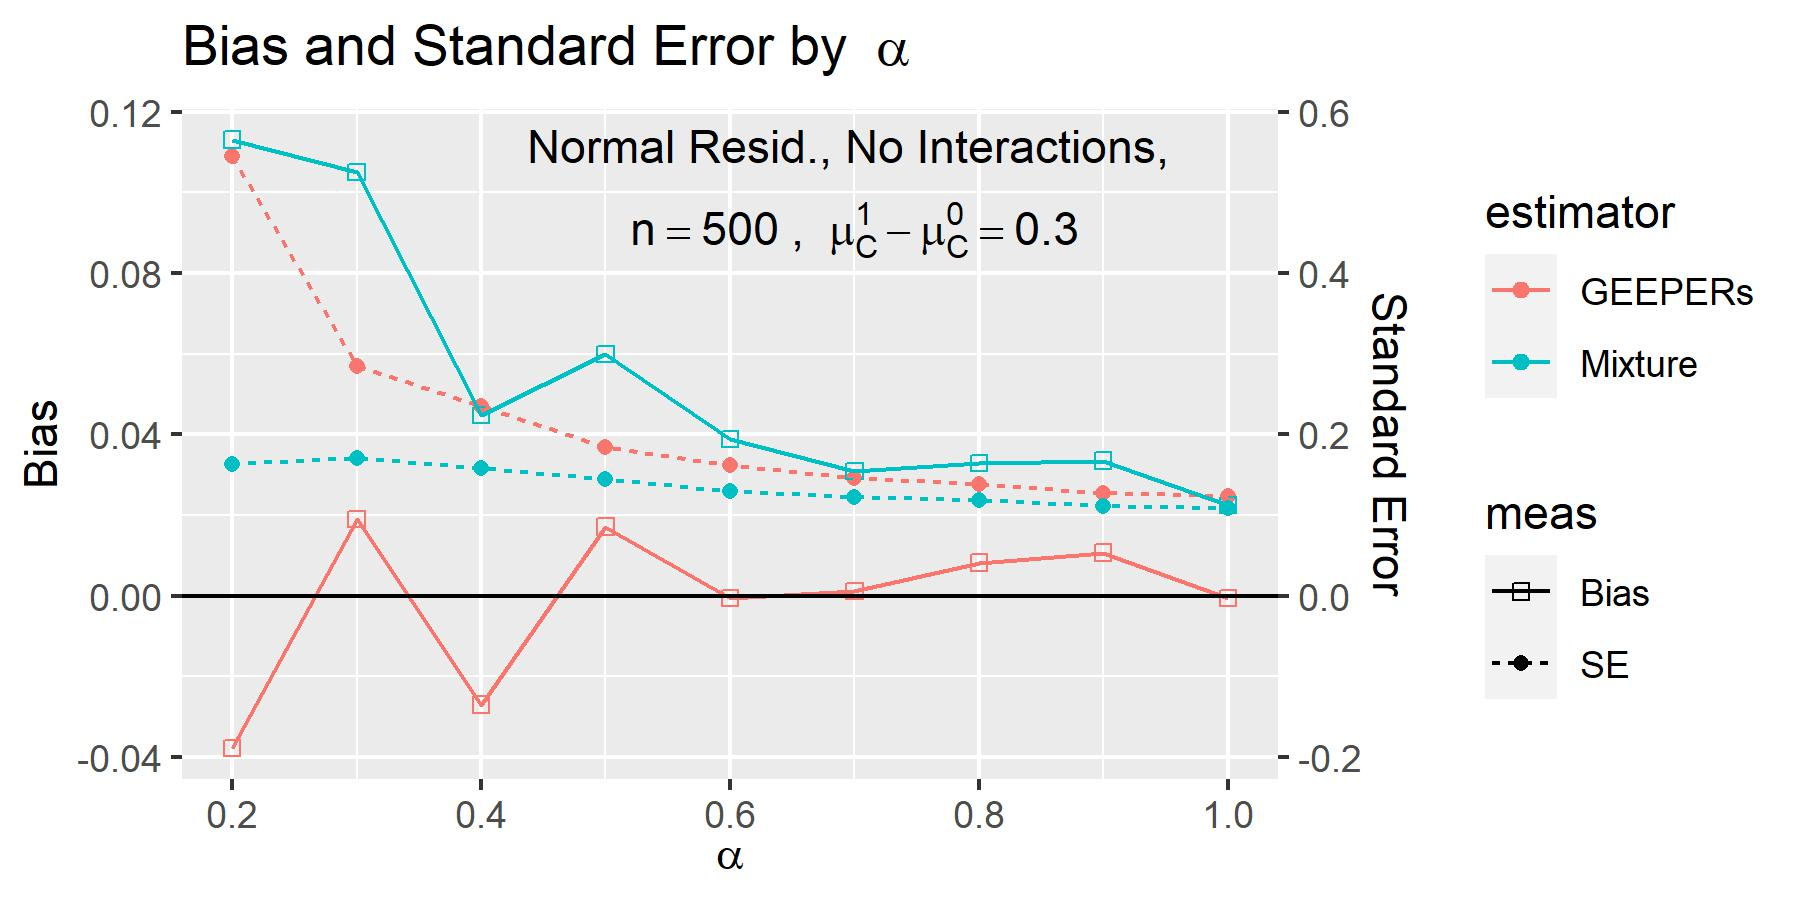
\includegraphics{../simFigs/biasSEbyB1.jpg}
%   \caption{Empirical bias and standard error of M- and Mixture estimates of $\muc1$ as $\alpha$ varies from 0.1 to 1. There were 500 replications for each $n$. Other factors were held fixed at the noted values.}
%   \label{fig:alpha}
% \end{figure}

\subsubsection{Other Factors}


\begin{figure}[!ht]
  \centering
  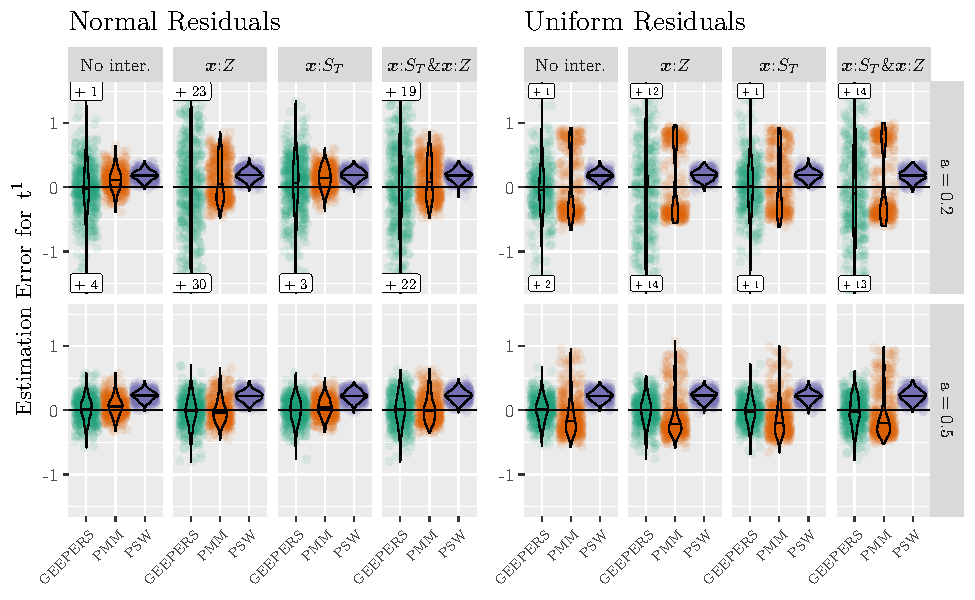
\includegraphics[width=5.5in,clip]{../simFigs/boxplotsNew.pdf}
  \caption{Violin and scatter plots of 500 simulation estimation errors for estimators described in Section~\ref{sec:simMods} under varying conditions. For all plots, $n=500$; there were 500 replications for each set of conditions. Annotations indicate the number of extreme outliers excluded from the plotting area.}
  \label{fig:boxplots}
\end{figure}

%<<<<<<< HEAD
Figure \ref{fig:boxplots} shows violin plots, layered on top of jittered scatter plots, showing estimation error for \textsc{geepers}, the parametric mixture model, and the \textsc{psw} estimator of $\eff1$ for, and Table \ref{tab:coverage} shows empirical coverage of nominal 95\% confidence interval estimates for \textsc{geepers} and a parametric mixture models; when at least one of an estimator's assumptions is violated, the result is colored red.

The first row of Table \ref{tab:coverage} and the first column of Figure \ref{fig:boxplots} show similar results as Figure \ref{fig:alphan}---when all assumptions of both methods are met, \textsc{geepers} is slightly less biased than the parametric mixture model; when $\alpha=0.2$, \textsc{geepers} is much more variable and $\alpha=0.5$ the difference in variance is slight.
\textsc{psw} has by far the lowest variance and the highest bias; the latter is due to the violation of principal ignorability. 

The remainder of the results reflect violations modeling assumptions for either \geepers or the parametric mixture model or both: interactions in the data generating model between covariates $X$ and treatment assignment $Z$ and/or principal stratum $S$, either of which would violate assumption \ref{ass:rci} and the linear additive model of the \textsc{pmm}, and/or residuals drawn from a uniform distribution, which violates the normality assumption of \textsc{pmm}.
For \geepers, when $\alpha=0.2$ the presence of interactions in the data-generating model increases sampling variance, but only interactions between $X$ and $Z$ reduce confidence interval coverage. When $\alpha=0.5$, the presence of interactions has little to no effect on the performance of the \geepers estimator, and all 95\% confidence intervals approximately achieve their nominal levels. \geepers makes no assumptions about the shape of the residual distribution and behaves similarly under either normal or uniform residuals.

Like \geepers, \pmm is insensitive to interactions between $X$ and $S$. However, interactions between $X$ and $Z$ in the data-generating model skew the \pmm sampling distribution and reduce the coverage of its 95\% confidence intervals, even when $\alpha=0.5$.
When the residual distribution was uniformly distributed, the \pmm sampling distribution appeared bimodal, and its credible intervals exhibited severe undercoverage.

\label{simsum}In sum, \psw is the least variable of all three estimators, and does not depend on outcome modeling, but is vulnerable to bias from an unmeasured covariate that predicts both $S$ and $Y$.
When all assumptions of both methods are met, \geepers is less efficient, but also less biased, than \pmm, but differences in efficiency decrease with $n$ and $\alpha$.
Neither \psw nor \pmm is vulnerable to interactions between $X$ and $S$.
\pmm is highly vulnerable to violations of normality and to interactions between $X$ and $Z$, while \psw is robust to non-normality and robust to $X$-$Z$ interactions when $\alpha = 0.5$.
These results suggest that researchers who are willing to assume principal ignorability should use \psw, and those who are confident in their parametric model for potential outcomes should use a parametric mixture model. Researchers who are hesitant to accept principal ignorability or a parametric outcome model should consider \geepers. 

\label{evalMetric}The simulation study suggests that none of the three methods evaluated---\geepers, \pmm, or \psw---dominates the others, and offers some guidance on when each estimator may be preferable. \psw is the most precise and requires no assumptions about the distribution of outcomes, but can be quite sensitive to violations of principal ignorability. When the determinants of $\st$ are well-understood and measured, \psw seems to be the best option. When principal ignorability does not hold, potential outcomes are conditionally normal, and there are no $X:Z$ interactions within principal strata, the \pmm estimator outperforms \geepers, though the difference decreases with $n$ or $\alpha$. \geepers may be the best choice when conditional normality may not hold, or if there are $X:Z$ interactions and $\bm{x}$ is sufficiently predictive of $\st$ (AUC $\ge$0.675, corresponding to $\alpha \ge 0.5$, may serve as a threshold). 
These suggestions may depend heavily on the simulation setup here; applying them in general scenarios requires more research. 


%=======
% Figure \ref{fig:boxplots} shows violin plots, layered on top of jittered scatter plots, showing estimation error for \textsc{geepers}, the mixture estimator, and the \textsc{psw} estimator of $\eff1$ under various sets of conditions, and Table \ref{tab:coverage} shows empirical coverage of nominal 95\% confidence interval estimates under a somewhat wider set of circumstances when $\muc1=0.3$. More complete results, including root-mean-squared-error estimates, are in the online appendix.
% The leftmost panel of Figure \ref{fig:boxplots} and the top line of Table \ref{tab:coverage} show results under conditions favorable to both the mixture model and to \textsc{geepers}---normal residuals and no interactions in the data generating model between covariates and either $S$ or $Z$.
% \textsc{geepers} was roughly unbiased, but less precise than the other two methods---when $\alpha=0.2$ it was much noisier, and when $\alpha=0.5$ it was only slightly less precise.
% The mixture estimator's bias depended on $\muc1$---when $\muc1=0$, the bias was slight, and when $\muc1=0.3$, the bias was more substantial. This result is somewhat surprising, because when $\muc1=0$, there was no separation between the principal strata in the control group, and previous literature \citep{griffin2008application} has identified this scenario as a particular challenge for mixture modeling.
% The \textsc{psw} estimator was also biased, due, presumably, to the violation of Principal Ignorability, Assumption \ref{ass:PI}, inherent in the data generating model. On the other hand, the \textsc{psw} estimator had easily the lowest sampling variance of the three estimators.

% The middle panel of Figure \ref{fig:boxplots} and the fifth line of Table \ref{tab:coverage} show results for when the residuals in \eqref{eq:y-sim} are uniformly distributed.
% In this case, \textsc{geepers} and \textsc{psw} estimators, which do not assume normality, behaved in a similar fashion as in the normal case, but the mixture estimator showed a bimodal pattern--sometimes over-estimating $\eff1$ and sometimes underestimating, but rarely estimating $\eff1$ accurately.
% Credible intervals from the mixture model exhibited severe undercoverage, while \textsc{geepers} confidence intervals achieved at least their nominal level.

% %\sloppy
% The rightmost panel of Figure \ref{fig:boxplots} returns to the case of normal residuals---and only shows results when $\muc1=0.3$ and $\alpha=0.5$---but introduces interactions in the data generating model between covariates and either $\st$, $Z$, or both, violating Assumption \ref{ass:rci}.
% %Presence of interactions could undermine the \textsc{geepers} by inducing a relationship between principal scores and potential outcomes, even after adjusting the outcomes for covariate effects.
% Fortunately, these interactions made little difference when $\alpha=0.5$. However, Table \ref{tab:coverage} shows that when $\alpha=0$ or 0.2, and interactions between $\bx$ and $Z$ were present (i.e., $\gamma_3\ne 0$), \textsc{geepers} 95\% confidence intervals tended to under-cover. Nevertheless, coverage of \textsc{geepers} intervals was nearly always substantially higher than coverage of corresponding 95\% credible intervals from mixture models.%\footnote{}
% >>>>>>> overleaf-2025-06-12-1948



\begin{table}%[!ht]

\caption{\label{tab:coverage}Empirical coverage of nominal 95\% confidence intervals for estimates of $\tau^1$.}
\centering
% \begin{tabular}[t]{lllllll}
% \toprule
% \multicolumn{3}{c}{ } & \multicolumn{2}{c}{$\alpha=0.2$} & \multicolumn{2}{c}{$\alpha=0.5$} \\
% \cmidrule(l{3pt}r{3pt}){4-5} \cmidrule(l{3pt}r{3pt}){6-7}
% \makecell[l]{Residual\\Dist.} & \makecell[l]{X:Z\\Int.?} & \makecell[l]{X:S\\Int.?} & \geepers & \pmm & \geepers & \pmm\\
% \midrule
%  & No & No & 0.97 & 0.97 & 0.96 & 0.96\\

%  & Yes & No & \rd{0.88} & \rd{0.74} & \rd{0.94} & \rd{0.89}\\

%  & No & Yes & \rd{0.98} & \rd{0.97} & \rd{0.97} & \rd{0.96}\\

% \multirow{-4}{*}{\raggedright\arraybackslash Normal} & Yes & Yes & \rd{0.9} & \rd{0.77} & \rd{0.94} & \rd{0.88}\\
% \cmidrule{1-7}
%  & No & No & 0.97 & \rd{0.4} & 0.95 & \rd{0.61}\\

%  & Yes & No & \rd{0.87} & \rd{0.2} & \rd{0.93} & \rd{0.48}\\

%  & No & Yes & \rd{0.98} & \rd{0.53} & \rd{0.96} & \rd{0.57}\\

% \multirow{-4}{*}{\raggedright\arraybackslash Uniform} & Yes & Yes & \rd{0.88} & \rd{0.21} & \rd{0.94} & \rd{0.53}\\
% \bottomrule
% \multicolumn{7}{p{3.5in}}{\footnotesize Based on 500 replications. $n=500$, $\beta_1=0.3$. Simulation standard error $\approx 1$ percentage point. Estimates colored \rd{red} indicate cases where the assumptions of the model are not met.}

% \end{tabular}
\begin{tabular}[t]{lllrrrrrr}
\toprule
\multicolumn{3}{c}{ } & \multicolumn{2}{c}{$\alpha=0$} & \multicolumn{2}{c}{$\alpha=0.2$} & \multicolumn{2}{c}{$\alpha=0.5$} \\
\cmidrule(l{3pt}r{3pt}){4-5} \cmidrule(l{3pt}r{3pt}){6-7} \cmidrule(l{3pt}r{3pt}){8-9}
\makecell[l]{Residual\\Dist.} & \makecell[c]{X:Z\\Int.?} & \makecell[r]{X:S\\Int.?} & GEEPERs & Mix.  & GEEPERs & Mix. & GEEPERs & Mix.\\
\midrule
 & No & No & 0.99 & 0.99  & 0.97 & 0.97 & 0.96 & 0.96\\

 & Yes & No & 0.88 & 0.74  & 0.88 & 0.74 & 0.94 & 0.89\\

 & No & Yes & 1.00 & 1.00  & 0.98 & 0.97 & 0.97 & 0.96\\
\multirow{-4}{*}{\raggedright\arraybackslash Normal} & Yes & Yes & 0.90 & 0.77  & 0.90 & 0.77 & 0.94 & 0.88\\
\cmidrule{1-9}
 & No & No & 0.99 & 0.29  & 0.97 & 0.40 & 0.95 & 0.61\\

 & Yes & No & 0.83 & 0.11  & 0.87 & 0.20 & 0.93 & 0.48\\

 & No & Yes & 1.00 & 0.47  & 0.98 & 0.53 & 0.96 & 0.57\\

\multirow{-4}{*}{\raggedright\arraybackslash Uniform} & Yes & Yes & 0.83 & 0.15 & 0.88 & 0.21 & 0.94 & 0.53\\
\bottomrule

\end{tabular}

\end{table}



\section{Applications}
To illustrate \textsc{geepers} and compare it to the other discussed methods, we include two applied examples.
First, we briefly replicate an analysis from \citet{richardson2023estimating} using the \textsc{geepers} and the other methods discussed above.
This is a relatively straightforward example of an experiment with imperfect compliance in which \citet{richardson2023estimating} estimated statistically significant effects overall in both principal strata.
Next, we present a novel analysis of data from the RCT of computer-based math applications reported in \citet{impactPaper}, and look into the role of bottom-out hints, as described in the introduction.
This analysis aims to shed light on an important question in education research, illustrates model and covariate selection, and includes a discussion on the plausibility of identification assumptions. 

\subsection{Accounting for Imperfect Compliance: Re-Analysis of the Obstetrics and Periodontal Therapy Study}
Periodontal disease, a weakening of bone and connective tissue supporting teeth, is highly prevalent among American adults and is associated with adverse pregnancy outcomes, including preterm birth \citep{periodontalEpi}.
The Obstetrics and Periodontal Therapy Study \citep[(OPTS)][]{michalowicz2006treatment} investigated the efficacy of nonsurgical periodontal treatment to reduce the preterm birth rate; replication data are available at \url{https://causeweb.org/tshs/obstetrics-and-periodontal-therapy/}.
Pregnant patients at four different hospitals who were at least 16 years old, at less than 16 weeks and 6 days of gestation, and diagnosed with periodontal disease were individually randomized to either receive periodontal treatment during the first 21 weeks of pregnancy ($Z=1$, $n_T=413$) or after delivery ($Z=0$, $n_C=410$).
The primary prespecified outcome of the study was the babies' gestational age at birth; however, the study team also collected data on several secondary birth outcomes, as well as measures of patients' periodontal disease at follow-up.

The main component of the intervention consisted of up to four visits, followed by monthly tooth polishing and other dental care as needed. However, not all participants randomized to the treatment condition completed the entire treatment plan.
However, 96\% of patients in the treatment group received at least some periodontal care during pregnancy---therefore, there is reason to suspect nonzero treatment effects even for those patients who did not (or would not) fully comply.
Patients randomized to the control condition did not have access to the intervention.
\citet{richardson2023estimating} used a method they refer to as ``bespoke instrumental variable'' (BSIV) to estimate the average effects for the principal stratum of subjects who, if randomized to treatment,  would complete the treatment plan and for the principal stratum of subjects who would not.
Here, we will use \textsc{geepers}, a Bayesian mixture model, and principal score weighting to estimate the same quantities, following the same analysis decisions as \citet{richardson2023estimating}.
Replication code for our analysis can be found at \url{ https://github.com/adamSales/psGee}.

Following \citep{richardson2023estimating}, we will estimate the principal effects of randomization $Z$ on $Y$, the percentage of probed sites (6 sites per tooth) that were bleeding at visit 5, which was at 29--32 weeks gestation, conditioning on two covariates, Serum measures of endotoxin level and fibrinogen at baseline.
We omit the 164 cases in which $Y$ was missing as well as 19 additional cases in which one or both of the covariates were missing, leaving a total sample size of 640, with 314 randomized to the treatment condition and 326 randomized to control.
The compliance variable in the dataset had three categories: ``Yes,'' for subjects in the treatment group who completed the treatment plan (157 subjects), ``No'' for those who did not (4 subjects), and ``Und'' for those who received some therapy, but it is unknown whether they completed the treatment (157 subjects).
We let $S=1$ when compliance was ``yes''---i.e., when subjects in the treatment group completed the treatment---and $S=0$ otherwise.

For all three estimation methods, we estimated principal scores with logistic regression of $\st$ on the two covariates.
For \textsc{geepers} and \textsc{psw}, we used standard maximum likelihood methods and data from the treatment group, achieving an AUC of 0.68. For the mixture model, we incorporated the logistic regression specification as a sub-model within a larger Bayesian model fit in Stan.

\begin{figure}
  \centering
  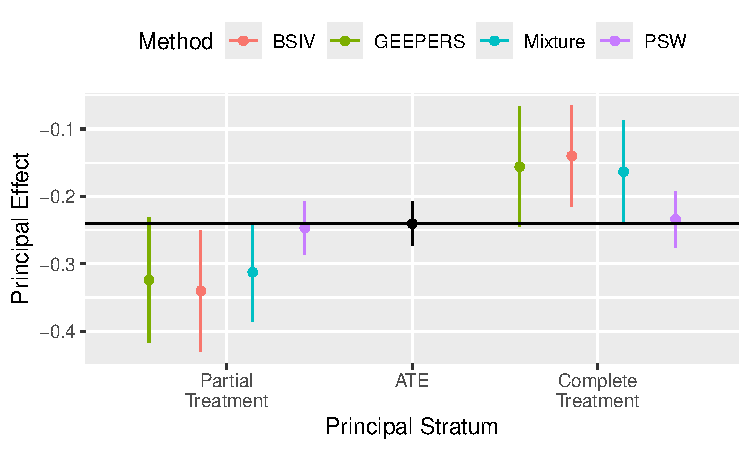
\includegraphics{figure/opts.pdf}
  \caption{Estimated principal effects and 95\% confidence or credible intervals for the Obstetrics and Periodontal Therapy Study, using four estimation methods. Results for BSIV were taken from \citet{richardson2023estimating}.}
  \label{fig:opt}
\end{figure}


The results are displayed in Figure \ref{fig:opt}% and Table \ref{tab:optEffs}
: both \textsc{geepers} and the Bayesian mixture model gave similar results to those reported in \citet{richardson2023estimating} from BSIV.
For the principal stratum of subjects who would not fully complete the treatment, those three methods estimated that assignment to the treatment condition reduced percentage of dental sites with bleeding by 31--34 percentage points; for subjects who would complete the treatment, the three estimated a reduction of 14-16 percentage points.
The conclusion of these methods is somewhat surprising: that the effect was larger for subjects who would not complete the treatment than for those who would (the two strata had similar bleeding percentages at baseline, and a logit transformation of the outcome leaves the results qualitatively unchanged). 
One possible explanation is the conjecture that subjects stop showing up for treatment once their periodontal disease has abated.

In contrast, principal score weighting resulted in very similar effects for both strata---a reduction of 23--25 percentage points, which is close to the estimated intent-to-treat effect of 25 percentage points.

\subsection{Estimating Treatment Effects for Implementation Subgroups: Students who Frequently or Rarely Request Bottom-Out Hints}\label{sec:fh2t}

In the educational field experiment reported in \citet{impactPaper}, middle school students completing their math schoolwork on a computer program were randomly assigned to four conditions.
These included two gamified programs---DragonBox and From Here to There (FH2T)---and two programs in which students used computers to work through a series of algebra problems taken from the district's textbook---``ASSISTments'' and an active control called ``Business as Usual'' (BAU).  % the active control condition in which students simply used the computer to work on a sequence of math problems.
In the DragonBox game, students learned to solve algebraic equations by isolating a box containing a dragon; as students progressed in the game, pictures of monsters were replaced by mathematical symbols.
Another condition, the From Here to There (FH2T) program, used visual cues such as color and spacing to teach algebraic concepts and allowed students to solve equations by manipulating expressions via dragging and dropping.
%In ASSISTments, students used computers to work through a series of math problems taken from the district's textbook.
Students in the ASSISTments condition had access to a series of hints for each problem, culminating in a ``bottom out'' hint that contained the answer. They received immediate feedback on their answers and had to enter the correct answer to proceed to the next problem.
In the BAU condition, students had no access to hints and received feedback only after completing the assignment.

In all four conditions, students worked on their assigned math program in class on 12 different occasions spaced throughout the school year: a prior assessment, a mid-test, a post-test, and nine learning sessions.
In this illustration, we will compare ASSISTments---the only condition featuring bottom-out hints---with each of the three others separately. Our goal is to estimate different treatment effects for groups of students who, if assigned to ASSISTments, would request few or many bottom-out hints.

The ability to bottom out was only one of several differences between the treatment conditions. One way to disentangle the role of bottoming out in any treatment effect would be to estimate average treatment effects of being assigned to ASSISTments, relative to any of the other three, separately for subjects who would (if assigned to ASSISTments) bottom out frequently, and for subjects who would not.
If the availability of bottom-out hints plays a positive role in ASSISTments' efficacy, we might expect larger effects of the condition on students who frequently bottom out than on those who do not; if bottom-out hints are harmful, we might expect the opposite.
If hints (that do not supply the correct answer) and error messages are helpful, but the ability to bottom out is harmful to learning, then we might expect to estimate a positive effect of being assigned to the feedback condition for students who do not bottom out, but a negative effect for students who do. If hints are helpful for learning only if they can be read as worked examples, then we might expect no effect of condition on students who generally do not bottom out, but a positive effect for students who do.
(These hypothetical results may be masked by other treatment effect heterogeneity between students who would or wouldn't bottom out, but the results could still be informative.)

\subsubsection{Principal Stratification and Alternatives}
The goal of principal strafication in this context is to determine if assignment to the ASSISTments condition affected students who tend to request frequent bottom-out hints differently than students who tended to request fewer bottom-out hints.
Is this the right question to ask?

In a similar context, \citet{sales2021student} suggests two alternative approaches: the average effect of requesting bottom-out hints on posttest scores for students in the ASSISTments condition, and estimating natural direct and indirect effects of assignment to the ASSISTments condition, treating bottom-out hint requests as a mediator.
The former approach is an observational study: although students were randomized to the ASSISTments condition, bottom-out hint requests were not randomized. Therefore, estimating the effect of bottom-out hints requires careful control of confounding.
Unfortunately, confounding is a major concern in this case, since, presumably, students only requested bottom-out hints if they were struggling with the material, and students who struggled with practice problems are likely to score lower on the posttest, on average, than those who needed less help during practice.
The best available measure of students' baseline ability, their score on the 10-item pretest, is likely insufficient.
That said, a plausible estimate of the average effect of bottom-out hint requests would be a valuable contribution to the literature, and a suitably innovative observational design \citep[e.g.][]{beck} may bear fruit.

Another arguable disadvantage of the observational study approach is that it overlooks the broader context of the experiment, focusing on whether bottom-out hints affect posttest scores rather than examining their role in ASSISTments' overall effectiveness.
A second approach, mediation analysis, contextualizes the bottom-out effect within the larger experiment.
It, too, relies on the same non-confounding assumption as an observational study, and also suffers from an additional challenge: mediation analysis relies on a ``common support'' condition that ``the mediator state must not be a deterministic function of the treatment'' \citep[p. 225]{celli2022causal}.
However, bottom-out hints are unavailable in the other three arms of the study, violating this condition (\citealt{sales2021student} offers a solution, which we find unconvincing).

A principal stratification approach treats bottom-out hint requests as a type of compliance.
In other words, if we consider full implementation of the ASSISTments condition to include frequent bottom-out hint requests, students assigned to ASSISTments but who requested few bottom-out hints only partially complied with their treatment assignment.
The question then is whether students who do not fully comply with their treatment assignment still experience an effect.
Conversely, might students who only partially comply experience a larger positive effect?
That would be the case if either bottom-out hints were harmful or if the treatment was better targeted toward the type of student who tends to need them less.

Principal score weighting depends on the assumption of principal ignorability, which is equivalent to the no-confounding assumption of the observational study and mediation analysis.
The mixture model and \textsc{geepers} estimators do not rely on that assumption, instead relying on parametric models and residualized covariate independence, respectively.
Finally, the instrumental variables estimator of \citet{air} relies on the ``exclusion restriction'' that, for students who request few bottom-out hints, there is no effect of randomization to the ASSISTments condition.
Since bottom-out hints are only one of several features of ASSISTments, this assumption is untenable. 


\subsubsection{Data on Bottom-Out Hints and Covariates}

\sloppy
We gathered dichotomized data on %which students in the treatment condition requested at least one bottom-out hint.
whether students in ASSISTments requested more than the median number of bottom-out hints (i.e., 11).
That is, $\st=1$ for students who, if assigned to ASSISTments, would request more than 11 bottom-out hints (``bottom-outers''), and $\st=0$ for students who would request 11 or fewer (``non-bottom-outers''). %least one bottom-out hint, and $\st=0$ for students who would not.
The outcome of interest $Y$ in our example is students' total scores on a ten-item posttest completed within the online tutoring system; $Y$ is an integer ranging from 0 to 10.
The goal of our analysis will be to determine the principal effects $\eff1=\EE[\yt-\yc|\st=0]$ and $\eff0=\EE[\yt-\yc|\st=0]$, the average effects of assignment to ASSISTments (``$T$'' subscripts) versus the other conditions (``$C$'') for bottom-outers and non-bottom-outers.

We also had access to data on several baseline covariates, including prior achievement, demographics, baseline measurements of student attitudes toward math, and an indicator for whether students began the school year in remote or in-person instruction.
Students with missing pretest scores were dropped from the analysis; missing data in other covariates were imputed with a Random Forest algorithm \citep{missForest}. Summary statistics are displayed in appendix tables \ref{table:tab1fac} and \ref{table:tab1num}.

%The data analysis we present here is intended as a demonstration of \textsc{geepers}, rather than for its substantive conclusions, and our description omits discussion of some important methodological considerations, including attrition and post-selection inference.
For details on the experimental design, the conditions being compared, sample attrition---which was unusually high due to the COVID-19 pandemic---and the impact analysis, please see \citet{impactPaper}.

For a description of the dataset and an explanation of how to access it, see \citet{ottmar2023data} and \url{https://osf.io/r3nf2/}.
Replication code for the analysis is available at %[Redacted].
\url{https://github.com/adamSales/psGee}.

\subsubsection{Data Analysis}
We estimated principal scores using logistic regression of observed $S$ on school fixed effects and a set of baseline variables $\bxs$.
Three criteria governed our choice of covariates and regression specifications for estimating principal scores and effects.
First, Proposition \ref{prop:reg2} requires consistent estimation of principal scores and (via Assumption \ref{ass:rci}) correct specification of the outcome model, that is, the model for $\EE[Y|\bxy,Z,\st]$.
Hence, it is essential to choose covariates and transformations $\bxs$ and $\bxy$ that lead to a good model fit.

Second, Assumption \ref{ass:vps} requires principal scores to vary with at least some element $\bxs$. Moreover, the results of the simulation study suggest that when $\st$ can be predicted more precisely as a function of $\bxs$, \textsc{geepers} principal effect estimators are more precise and more robust to model misspecification.
Those considerations militate in favor of choosing covariates $\bxs$ to optimize out-of-sample principal score prediction accuracy.

There is good reason to believe that analogous arguments apply to the selection of outcome covariates $\bxy$.

The first two criteria motivated our choice of two strategies for choosing $\bxs$ and $\bxy$.
In our main model, we included every available covariate in the dataset and chose transformations of those covariates based on the results of residual and binned residual plots \citep{arm}.

Including all possible covariates maximizes the model's opportunities to detect covariate relationships that would predict $Y$ or $\st$.
However, this strategy can also lead to overfitting, which would decrease out-of-sample predictive accuracy.
In an alternative analysis, we chose a subset of covariates to include in $\bxs$ and $\bxy$ with a backward stepwise selection algorithm minimizing the AIC \citep{aic} of the principal score model and then modified the resulting models based on residual plots.
The model selection process is recorded in the GitHub repository cited above.

Lastly, Assumption \ref{ass:ci} implies that there is no interaction between $\bxs$ and $\st$ in the outcome model. Further, for the sake of statistical efficiency, we did not consider outcome models with interactions between covariates and $Z$.
\emph{A priori}, the student attribute that poses the greatest threat to these modeling choices is prior achievement, that is, scores on the pretest and the fifth-grade state test.
This is both because they measure a similar construct to the posttest, and because \cite{impactPaper} found a pretest-treatment interaction in a different treatment contrast.
Following that reasoning, we conducted a third parallel analysis excluding prior achievement covariates.% in $\bxs$ but including all covariates in $\bxy$.

All three principal score models were fit to data from students in the ASSISTments group, for whom bottom-out status ($S$) was observed; hence, the same model fit was used for all three treatment contrasts.

Outcome models for all analyses adjusted for all of the variables that were in the corresponding principal score models, in addition to measurements of students' prior knowledge; also, the models substituted class fixed effects for school fixed effects.\footnote{Why use a coarser set of fixed effects for the principal score model than the outcome regression? First, the principal score model was fit to a smaller sample (only students in the ``Instant'' condition), so some classrooms only included one student, which can lead to poor fit. Second, the asymptotics of logistic regression are more restricted than OLS, so logistic regression tends to perform poorly when the number of parameters increases with the sample size \citep{agresti}.}
As with principal score models, we checked model fit with residual plots and modified model specifications accordingly.


% \begin{figure}
%   \centering
%   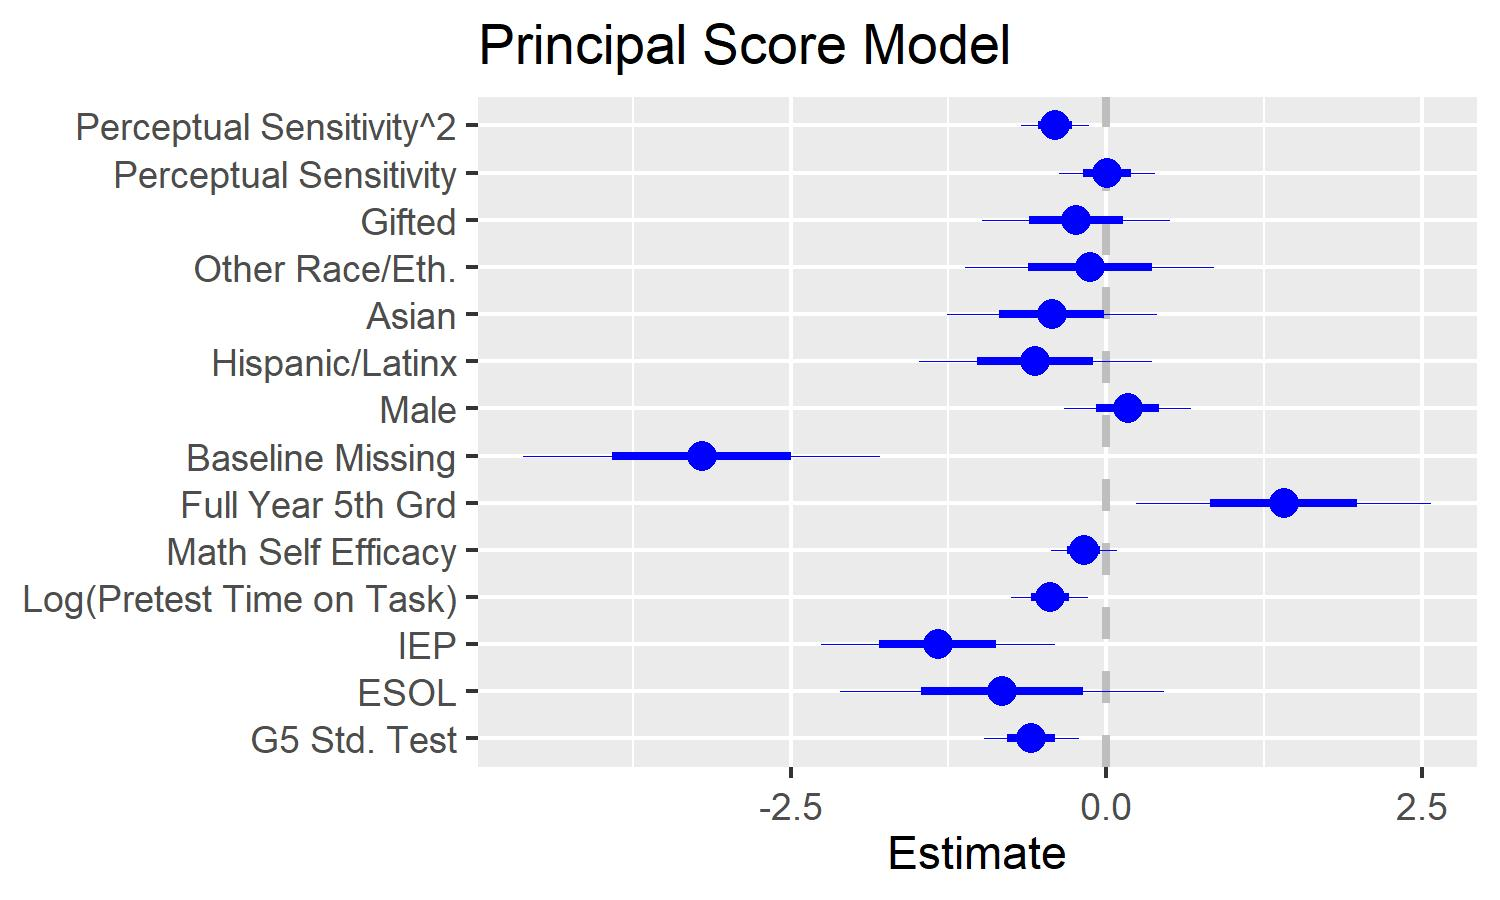
\includegraphics{../figure/psModCoef.jpg}
%   \caption{Principal Score Model Coefficients}
%   \label{fig:psMod}
% \end{figure}

\subsubsection{Results}

The three principal score models were fairly successful in distinguishing bottom-outers from non-bottom-outers---the AUC, evaluated using out-of-sample predictions in a 10-fold cross-validation, was roughly 0.795 for the AIC-optimal model, and about 0.745 for the two others. That is, in roughly 75--80\% of bottom-outer/non-bottom-outer pairs of subjects, the bottom-outer will have a higher predicted probability from the model.
Coefficient estimates are displayed in Table \ref{tab:psTab} in the appendix.

Figure \ref{fig:effects} shows principal effect point estimates and 95\% confidence intervals from analyses based on the three principal score models.
The three covariate selection strategies led to similar point and interval estimates.
That said, in nearly all cases, the AIC-optimal model led to the smallest standard errors.
Confidence intervals for all nine principal effect estimates were about twice as wide as for corresponding ATE estimates.
In no case was there evidence at $\alpha=0.05$---or any other conventional level---for non-zero principal effects or differences between principal effects.
Table \ref{tab:regTab}, in the appendix, displays the full set of regression coefficients for the outcome models based on the "All Covariates" principal score model, along with nominal standard error estimates.

A comparison of point estimates suggests that assignment to ASSISTments rather than BAU benefits bottom-outers less than non-bottom-outers.
We speculate that, if true, this pattern may be because many students use bottom-out hints to game the system---entering the provided correct answers rather than attempting to figure out the problems on their own.
Removing access to hints for bottom-outers forces them to attempt the problems rather than game the system.
At the same time, hints and instant feedback are helpful for non-bottom-outers, who are less likely to game the system.

On the other hand, point estimates suggest that assignment to ASSISTments, relative to FH2T, hurts non-bottom-outers but not non-bottom-outers.
Perhaps non-bottom-outers tend to have higher prior knowledge, and, as \cite{impactPaper} shows, FH2T benefits such students more than students with lower prior knowledge.

Perhaps the simplest explanation for observed differences in point estimates is sampling error, which cannot be ruled out.

\begin{figure}
  \centering
  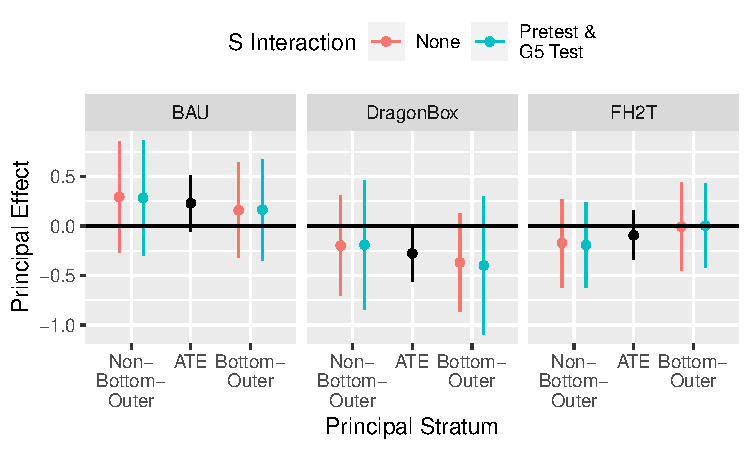
\includegraphics{figure/prinEffs.pdf}
  \caption{Principal effect estimates with 95\% confidence intervals using three different principal score models, alongside ATE estimates and 95\% confidence intervals, for contrasts between the ASSISTments condition and each of the three other conditions in the study.}
  \label{fig:effects}
\end{figure}

\subsubsection{Comparing Principal Stratification Methods}


\begin{figure}
  \centering
  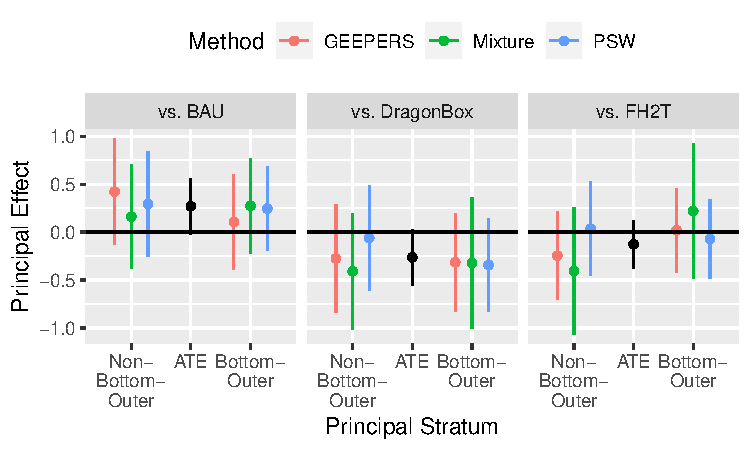
\includegraphics{figure/compareMethods.pdf}
  \caption{Principal effect estimates with 95\% confidence or credible intervals using three different principal stratification methods, alongside ATE estimates and 95\% confidence intervals, for contrasts between the ASSISTments condition and each of the three other conditions in the study. The \textsc{geepers} estimates used the ``All Covariates'' principal score model.}
  \label{fig:compare}
\end{figure}

Figure \ref{fig:compare} shows principal effect estimates from \textsc{geepers} (using the All Covariates principal score model) compared to analogous estimates using Bayesian mixture modeling and \textsc{psw}, alongside estimates of the overall average treatment effects, labeled ``ATE.''

The \textsc{psw} model used the same principal score model as \textsc{geepers}, while the Bayesian model used the same principal score and outcome model specifications.

The Bayesian mixture model assumed that outcomes were normally distributed, conditional on covariates and principal stratum, with a residual standard deviation that varied between principal strata. This modeling assumption is necessarily false since post-test scores were integers between 0 and 10. All model parameters with support in $\mathbb{R}$ were given standard normal priors, while standard deviation parameters were given half-standard normal priors.
The principal score and outcome models were fit simultaneously using a Markov Chain Monte Carlo algorithm \citep{rstan}.

The \textsc{psw} estimators did not include any covariate outcome modeling. Standard errors for the \textsc{psw} estimates were estimated using the bootstrap, with resampling done within schools.

For all three sets of estimators, approximate 95\% confidence intervals were estimated by adding and subtracting twice the standard error from the point estimate (or twice the posterior standard deviation from the posterior mean, in the Bayesian mixture model).

The other estimation strategies largely agreed with \textsc{geepers} and with each other in the contrast between ASSISTments and BAU, and, to a lesser extent, in the contrast between ASSISTments and DragonBox. The biggest difference between the methods was in the contrast with FH2T, in which the Bayesian mixture model resulted in a larger difference between the two principal effects, as well as the largest standard errors, while the two \textsc{psw} principal effect estimates were quite similar.  However, these differences are difficult to interpret due to the large uncertainty around all of the point estimates.

\section{Discussion}\label{sec:discussion}
\textsc{geepers} is a straightforward approach to principal effect estimation under strong monotonicity, built on widely-used regression models, which is more robust---though sometimes less precise---than alternative approaches under a wide array of scenarios.

There is good reason to hope that extensions to \textsc{geepers}, including cases in which $S$ takes more than two values, may be straightforward.
For instance, in truncation by death problems \citep[e.g.][]{zhangRubin,ding2011} with weak monotonicity, $S_i=1$ if participant $i$ survives (or, more generally, if the outcome $Y_i$ is measured) and 0 otherwise, interest is typically in the principal effect for the ``always survive'' principal stratum in which $\sti=S_{ci}=1$.
If, say, $\sti\ge S_{Ci}$, then every subject in the control condition with $S_i=1$ is in the always survive stratum, while those subjects in the treatment condition with $S_i=1$ are a mixture of the always survive and $\sti=1;\;S_{Ci}=0$ stratum.
This scenario is broadly similar to the strong monotonicity, one-way noncompliance situation that this paper discussed.
On the other hand, when no monotonicity assumption holds, both $\st$ and $S_C$ will have to be imputed for every subject; further research is necessary to determine the appropriate way to do so.

Another direction of extension involved the principal score model \eqref{eq:pscore}.
The performance of \textsc{geepers} in the simulation study of Section \ref{sec:simulation} depended heavily on the factor $\alpha$, which controlled the extent to which covariates could predict $S$.
That suggests that when covariates are high-dimensional, \textsc{geepers}' performance in applications could be optimized with a high-dimensional semi- or non-parametric model.
If so, several further questions emerge.
First, can the parameter $\alpha$ be extended to a more general parameter measuring the prediction accuracy of a non-parametric model?
Second, if the principal score model cannot be formulated as the solution to a set of estimating equations, how should the standard error be computed?
Lastly, can over-fit principal score models cause bias or other estimation problems, and if so, are there ways to protect against overfitting?

Sampling error prevents firm conclusions regarding principal effects for students who would, if given the opportunity, request frequent bottom-out hints.
However, the results are consistent with the hypothesis that ASSISTments is less effective for frequent bottom-out requesters when compared to a similar program without hints or immediate feedback. We hypothesize that many students who request bottom-out hints frequently are gaming the system, abetted by the availability of bottom-out hints.

\textsc{geepers} is a flexible, easily-implementable method for principal effect estimation for one-way noncompliance, with predictive covariates; extensions to a broader set of circumstances could be a boon to causal modeling.

\bibliographystyle{apalike}
\bibliography{MOM}




\appendix

\section*{Appendix: Proofs and Calculations}
\subsection*{Proof for Lemma \ref{lemma:expectation}}
As a preliminary, note that
% \begin{align*}
%   \EE[\st|\hpp]&=\EE\left\{\EE[\st|\pp,\hpp]|\hpp\right\}\\
%              &=\EE\left\{\EE[\st|\pp]|\hpp\right\}\\
%              &=\EE[\pp|\hpp]=\hpp
% \end{align*}

%Then, note
\begin{align*}
  \EE[Y_C|\pp]&=\EE\left\{\EE[Y_C|\pp,\st]|\pp\right\}\\
             &=\EE\left\{\EE[Y_C|\st]|\pp\right\}\tag*{by \eqref{eq:assumption}}\\
             &=\EE[\muc1\st+\muc0(1-\st)|\pp]\\
             &=\muc1\pp+\muc0(1-\pp)
\end{align*}

Then we have
\begin{equation*}
  \begin{split}
    \EE[Y_C]=&\EE\EE[Y_C|\pp]=\muc1\EE\pp+\muc0(1-\EE\pp)\\
    =&\muc0+\EE\pp(\muc1-\muc0)
    \end{split}
\end{equation*}

Next we have

\begin{align*}
  \EE[Y_C\pp]&=\EE\left\{\EE[Y_C\pp|\pp]\right\}\\
            &=\EE\left\{\pp\EE[Y_C|\pp]\right\}\\
            &=\EE\left\{\pp\left[\muc1\pp+\muc0(1-\pp)\right]\right\}\\
            &=\EE[\pp]\muc0+\EE[\pp^2](\muc1-\muc0)
\end{align*}

In the treatment group, $\st$ is observed, so
\begin{align*}
    \EE[Y_T]=&\mut0+\EE[\st](\mut1-\mut0)\tag*{and}\\
    \EE[\st Y_T]=&\EE[\st]\mut0+\EE[\st^2](\mut1-\mut0)
\end{align*}

Due to Assumption \ref{ass:rand} (randomization), $\EE[Y|Z=0]=\EE[Y_C]$, $\EE[Y|Z=1]=\EE[Y_T]$, $\EE[Y\pp|Z=0]=\EE[Y_C\pp]$ and $\EE[YS|Z=1]=\EE[Y_T\st]$, completing the proof.

\subsection*{Proof for Proposition \ref{prop:reg1}}

Replacing $\sti$ and $\pp$ in \eqref{eq:estEq0} with $\ri$, as in \eqref{eq:ri}, and replacing $\tilde{\Psi}_i$ with $\Psi_i=\begin{psmallmatrix} 1 & 0&1&0\\ 0&1&0&1\\0&0&1&0\\0&0&0&1\end{psmallmatrix}\tilde{\Psi}_i$ gives an equivalent set of estimating equations $\sum_{i=1}^{n_C}\Psi_i=\bm{0}$ with $\Psi_i=$
\begin{equation}\label{eq:estEq1}
\begin{pmatrix}
    Y_i-\muc0-\ri(\muc1-\muc0)-Z_i(\mut0-\muc0)-Z_i\ri(\mut1-\mut0-\muc1+\muc0)\\
    \ri Y_i-\ri\muc0-\ri^2(\muc1-\muc0)-Z_i\ri(\mut0-\muc0)-Z_i\ri^2(\mut0-\mut1-\muc0+\muc1)\\
    Z_iY_i-Z_i\mut0-Z_i\ri (\mut1-\mut0)\\
    Z_i\ri Y_i -Z_i\ri\mut0-Z_i\ri^2(\mut1-\mut0)

\end{pmatrix}
\end{equation}
These are equivalent to the estimating equations for OLS model \eqref{eq:regression0} with $\beta_0=\muc0$, $\beta_1=\muc1-\muc0$, $\beta_2=\mut0-\muc0$, and $\beta_3=\mut1-\mut0-\muc1-\muc0$.
Therefore, under standard OLS regularity conditions the estimated parameter vector $\bm{\hat{\beta}}$ is consistent, completing the proof.


\subsection*{A Stronger Version of Proposition \ref{prop:reg2} and a Proof}



\begin{prop}\label{prop:interactions}
  Say, for $i=1,\dots,n$, principal scores $\ppi$ are generated as \eqref{eq:pscore}, with parameters $\bm{\alpha}$ identified and consistently estimable with M-estimation, and there exist $\beta_0$, $\beta_1$, $\beta_2$, $\beta_3$, $\bm{\gamma_1}$, $\bm{\gamma_2}$, $\bm{\gamma_3}$ and $\bm{\gamma_4}$ such that $\{Y_i,Z_i,\sti,\bxy_i\}_{i=1}^n$ are independent and identically distributed with
  \begin{equation}\label{eq:interaction}
    \begin{split}
    \EE[Y_i|\st,Z,\bx]=&\beta_0+\beta_1\sti+\beta_2 Z_i+\beta_3Z_i\sti\\
    &+\bm{\gamma_1}'\bxy_i+\bm{\gamma_2}'\bxy_i\sti+
    \bm{\gamma_3}'\bxy Z_i+\bm{\gamma_4}'\bxy_i Z_i\sti
    \end{split}
  \end{equation}

  Then, under Assumptions \ref{ass:sm}, \ref{ass:rand}, and \ref{ass:vps}, if $\ppi$ is linearly independent of $\bxy$, a researcher may follow the following procedure to estimate principal effects:
  \begin{enumerate}
  \item Estimate principal scores by fitting model \eqref{eq:pscore} to data from the treatment group
  \item Replace $\sti$ with $\ri$ (as defined in \ref{eq:ri}) in model \eqref{eq:interaction} and fit with OLS
  \item Estimate principal effects as:
   \begin{equation}\label{eq:prinEffEstApp}
  \begin{split}
    \heff0_{int}&\equiv \hat{\beta}_2+\bm{\hat{\gamma}_3}'\overline{\bxy}_{Z=1,S=0}\\
    \heff1_{int}&\equiv \hat{\beta}_2+\hat{\beta}_3+(\bm{\hat{\gamma}_3}+\bm{\hat{\gamma}_4})'\overline{\bxy}_{Z=1,S=1}
  \end{split}
   \end{equation}
   where $\overline{\bxy}_{Z=1,S=0}$ and $\overline{\bxy}_{Z=1,S=0}$ are the vector of covariate sample means for the subsets of subjects with $Z=1$ and $S=0$ or $S=1$, respectively.
  \end{enumerate}
  Then $\heff0_{G}$ and $\heff1_{int}$ are M-estimators. If the estimating equations for \eqref{eq:prinEffEstApp} are each bounded by an integrable function of $\{\bm{Y},\bxy, \bm{S},\pp,\bm{Z}\}$ that does not depend on $\{\bm{\beta},\bm{\gamma}\}$, then $\heff0_{int}\rightarrow_p\eff0$ and $\heff1_{int}\rightarrow_p\eff1$ as $n\rightarrow\infty$.

  If the parameter estimates of the principal score model are asymptotically normal, second partial derivatives of the estimating equations for \eqref{eq:prinEffEstApp} are bounded by an integrable function of the data for values of $\{\bm{\beta},\bm{\gamma}\}$ in a neighborhood of their probability limits, and the sandwich components of \eqref{eq:sandwich}, $A$ and $B$, exist and are finite, and if $B$ is non-singular, then $\heff0_{int}$ and $\heff1_{int}$ are jointly asymptotically normal, with a variance of the form \eqref{eq:sandwich}.
\end{prop}

Equation \eqref{eq:interaction} implies Assumption \ref{ass:rci} with $\bm{\gamma_2}=\bm{\gamma_3}=\bm{\gamma_4}=0$.

\begin{proof}
First of all, by \eqref{eq:interaction},
\begin{equation*}
\begin{split}
  \EE[Y_T-Y_C|\st=0]&\\
  =&\EE[Y|Z=1,\st=0]-\EE[Y|Z=1,\st=0]\\
  =&\beta_2+\bm{\gamma_3}'\EE[\bxy|\st=0]
\end{split}
\end{equation*}
and
\begin{equation*}
\begin{split}
  \EE[Y_T-Y_C|\st=1]&\\
  =&\EE[Y|Z=1,\st=1]-\EE[Y|Z=1,\st=1]\\
  =&\beta_2+\beta_3+(\bm{\gamma_3}'+\bm{\gamma_4}')\EE[\bxy|\st=1]
\end{split}
\end{equation*}
Furthermore, $\overline{\bxy}_{Z=1,S=0}\rightarrow \EE[\bxy|\st=0]$ and $\overline{\bxy}_{Z=1,S=1}\rightarrow \EE[\bxy|\st=1]$ as $n\rightarrow \infty$.

We will show that the estimated coefficients from model \eqref{eq:interaction}, but with $R$ replacing $\st$, fit with OLS, are consistent for $\bm{\beta}$ and $\bm{\gamma}$ from \eqref{eq:interaction}.

First, note that $\EE[S]=\EE\EE[S|\bx]=\EE[\pp]$ and
\begin{align*}
  \EE[\bx S]&=\EE[\bx S|Z=1]=\EE[\bx S|Z=0] \mbox{ (due to randomization)}\\
  &=\EE[\bx\EE[S|\bx]|Z=0]=\EE[\bx\pp|Z=0]=\EE[\bx\pp]
\end{align*}
implying that, according to \eqref{eq:interaction},
\begin{equation*}
  \begin{split}
    \EE[Y|\bx,Z=0]&=\beta_0+\beta_1\pp+\bm{\gamma_1}'\bm{X^Y}+\bm{\gamma_2}'\bm{X^Y}\pp\\
                  &=\beta_0+\beta_1R+\bm{\gamma_1}'\bm{X^Y}+\bm{\gamma_2}'\bm{X^Y}R\\
    \EE[Y|\bx,S,Z=1]&=\beta_0+\beta_2+(\beta_1+\beta_3)S+(\bm{\gamma_1}+\bm{\gamma_3})\bxy+(\bm{\gamma_2}+\bm{\gamma_4})\bxy S\\
    &=\beta_0+\beta_2+(\beta_1+\beta_3)R+(\bm{\gamma_1}+\bm{\gamma_3})\bxy+(\bm{\gamma_2}+\bm{\gamma_4})\bxy R
  \end{split}
\end{equation*}
Therefore,
\begin{align*}
  \EE[Y]=&\EE[Y|Z=0]+\EE[Z]\left\{\EE[Y|Z=1]-\EE[Y|Z=0]\right\}\\
  =&\beta_0+\beta_1\EE[R]+\beta_2\EE[Z]+\beta_3\EE[ZR]+\bm{\gamma_1}'\EE[\bxy]+\bm{\gamma_2}'\EE[\bxy R]\\
  &+\bm{\gamma_3}'\EE[\bxy Z]+\bm{\gamma_4}\EE[\bxy RZ]
\end{align*}

Analogous reasoning leads to expressions for $\EE[RY]$, $\EE[\bxy Y]$, $\EE[ZY]$,  $\EE[ZRY]$, $\EE[\bxy YZ]$, and $\EE[\bxy RZY]$.
These, in turn, give rise to estimating equations
\begin{equation*}
\begin{split}
  &\psi_i=\\ &\begin{pmatrix}
  Y_i\\
  \phantom{}\\
  Y_i\ri\\
    \phantom{}\\
  Y_iZ_i\\
  \phantom{}\\
  Y_iZ_i\ri\\
  \phantom{}\\
  Y_i\bxy_i\\
  \phantom{}\\
  Y_i\bxy_i\ri\\
  \phantom{}\\
  Y_i\bxy_iZ_i\\
  \phantom{}\\
  Y_i\bxy_iZ_i\ri\\
  \phantom{}\end{pmatrix} - \begin{pmatrix*}[l]
    \beta_0+\beta_1R_i+\beta_2Z_i+\beta_3Z_iR_i\\
    \quad+\left\{\bm{\gamma_1}'+R_i\bm{\gamma_2}'+Z_i\bm{\gamma_3}'+R_iZ_i\bm{\gamma_4}'\right\}\bxy\\
    \beta_0\ri+\beta_1R_i^2+\beta_2Z_i\ri+\beta_3Z_iR_i^2\\
    \quad+\ri\left\{\bm{\gamma_1}'+R_i\bm{\gamma_2}'+Z_i\bm{\gamma_3}'+R_iZ_i\bm{\gamma_4}'\right\}\bxy\\
    (\beta_0+\beta_2)Z_i+(\beta_1+\beta_3)R_iZ_i\\
    \quad+Z_i\left\{\bm{\gamma_1}'+R_i\bm{\gamma_2}'+Z_i\bm{\gamma_3}'+R_iZ_i\bm{\gamma_4}'\right\}\bxy\\
    \beta_0Z_i\ri+(\beta_1+\beta_3)Z_iR_i^2+\beta_2Z_i\ri\\
    \quad+Z_iR_i\left\{\bm{\gamma_1}'+\bm{\gamma_3}'+R_i(\bm{\gamma_2}'+\bm{\gamma_4}')\right\}\bxy \\
    \beta_0\bxyt+\beta_1R_i\bxyt+\beta_2Z_i\bxyt+\beta_3Z_iR_i\bxyt\\
    \quad {}+\left\{\bm{\gamma_1}'+R_i\bm{\gamma_2}'+Z_i\bm{\gamma_3}'+R_iZ_i\bm{\gamma_4}'\right\}\bxy\bxyt\\
    \beta_0\ri\bxyt+\beta_1R_i^2\bxyt+\beta_2Z_i\ri\bxyt+\beta_3Z_iR_i^2\bxyt\\
    \quad {}+\ri\left\{\bm{\gamma_1}'+R_i\bm{\gamma_2}'+Z_i\bm{\gamma_3}'+R_iZ_i\bm{\gamma_4}'\right\}\bxy\bxyt\\
        (\beta_0+\beta_2)Z_i\bxyt+(\beta_1+\beta_3)R_iZ_i\bxyt\\
    \quad {}+Z_i\left\{\bm{\gamma_1}'+R_i\bm{\gamma_2}'+Z_i\bm{\gamma_3}'+R_iZ_i\bm{\gamma_4}'\right\}\bxy\bxyt\\
\beta_0\ri Z_i\bxyt+\beta_1R_i^2Z_i\bxyt+\beta_2\ri Z_i\bxyt+\beta_3Z_iR_i^2\bxyt\\
    \quad {}+\ri Z_i\left\{\bm{\gamma_1}'+R_i\bm{\gamma_2}'+Z_i\bm{\gamma_3}'+R_iZ_i\bm{\gamma_4}'\right\}\bxy\bxyt\\
  \end{pmatrix*}
  \end{split}
\end{equation*}
with $\EE[\psi_i]=0$.
These are the estimating equations for the regression model \eqref{eq:interaction}, with $R$ replacing $\st$, fit by OLS.
Consistency and asymptotic normality follow from theorems 7.8.1 and 7.8.2, respectively, of \citet{boosStefanskiBook}
\end{proof}

\subsection*{Sandwich Matrix Calculations}

Here we will derive the sandwich variance-covariance matrix for the \textsc{geepers} estimate without interactions between $\bx$ and either $Z$ or $\st$---i.e., with $\bm{\gamma_2}=\bm{\gamma_3}=\bm{\gamma_4}=0$ in the notation of \eqref{eq:interaction}---and estimating principal scores using a generalized linear model.

We propose estimating principal effects in two stages.
First, fit the model
\begin{equation}\label{eq:psMod}
  \ppi=Pr(\sti=1|\bxsi)=f(\bm{\alpha}'\bxsit)
\end{equation}
for some inverse link function $f(\cdot)$, where $\bxsit=[1,\bxsi]$, using (observed) values from the treatment group, and estimating $\hat{\alpha}$.
Then let
\begin{equation}\label{eq:ps}
  \hat{p}_i=f(\bm{\hat{\alpha}}'\bxsit)
\end{equation}
for all subjects in the experiment.

Finally, fit model
\begin{equation}\label{eq:regression}
  Y_i=\beta_0+\beta_1r_i+\beta_2Z_i+\beta_3Z_i\ri+\bm{\gamma}'\bxy_i+\epsilon_i
\end{equation}
to estimate $\bm{\beta}$ and hence principal effects, where $\bm{x}_i$ is a set of covariates predictive of $Y$ within principal strata.
Let $\bm{\beta}=[\beta_0,\beta_1,\beta_2,\beta_3,\bm{\gamma}']'$.

\sloppy
Following \eqref{eq:stacked}, let $\blam(Z_i,S_i,\bxsi,\bxy_i,Y_i;\bm{\alpha},\bm{\beta})=\begin{pmatrix} Z_i\Omega(\bxsi,S_i;\bm{\alpha})\\ \Psi(\bxy_i,\bxsi,Y_i,Z_i,\ri(\bm{\alpha});\bm{\beta})\end{pmatrix}$, the stacked estimating equations of \eqref{eq:psMod} and \eqref{eq:regression}.
Going forward, for the sake of brevity, we will write $\blam_i(\bm{\alpha},\bm{\beta})=\blam(Z_i,S_i,\bxsi,\bxy_i,Y_i;\bm{\hat{\alpha}},\bm{\hat{\beta}})$, where dependence on the data for $i$ is captured in the subscript $i$, with similar meanings for $\Psi_i(\bm{\alpha},\bm{\beta})$ and $\omega_i(\bm{\alpha})$.
%Then let $\blamh_i=\blam_i(Z_i,S_i,\bxsi,\bxy_i,Y_i;\bm{\hat{\alpha}},\bm{\hat{\beta}})$ be the estimating equations evaluated at the estimated parameters, and let

%\begin{equation*}
%\dblam_i=\frac{\partial}{\partial [\alpha,\beta]'} \blam_i\Bigr|_{\substack{\bm{\alpha}=\bm{\hat{\alpha}}\\\bm{\beta}=\bm{\hat{\beta}}}}
%\end{equation*}
%the derivative matrix of $\blam$ evaluated at the estimated parameters.

The variance-covariance matrix for $\bm{\hat{\alpha}}$ and $\bm{\hat{\beta}}$ can be estimated as:
\begin{equation*}
  \widehat{var}\left([\bm{\hat{\alpha}}',\bm{\hat{\beta}}']'\right)=A^{-1}BA^{-t}
\end{equation*}
where
\begin{equation*}%\label{eq:Amat}
  A=\sum_i \frac{\partial}{\partial [\bm{\alpha},\bm{\beta}]'} \blam_i\Bigr|_{\substack{\bm{\alpha}=\bm{\hat{\alpha}}\\\bm{\beta}=\bm{\hat{\beta}}}}
\end{equation*}
and
\begin{equation*}%\label{eq:Bmat}
  B=\sum_i \blam_i(\bm{\hat{\alpha}},\bm{\hat{\beta}})\blam_i(\bm{\hat{\alpha}},\bm{\hat{\beta}})'
\end{equation*}

Following \citet[][p. 373]{carroll2006measurement}, we %separate the estimating equations $\Psi$ into $\phi$ and $\psi$, estimating equations for models \eqref{
can decompose the matrices into diagonal elements
\begin{equation*}
    \begin{split}
        A_{1,1}&=\sum_i \partial \Omega_i/\partial \bm{\alpha}|_{\bm{\alpha}=\bm{\hat{\alpha}}}\\
        A_{2,2}&=\sum_i\partial\Psi_i/\partial \bm{\beta}|_{\bm{\beta}=\bm{\hat{\beta}}}\\
        B_{1,1}&=\sum_i\Omega_i(\bm{\hat\alpha})\Omega_i(\bm{\hat\alpha})'\\
        B_{2,2}&=\sum_i \Psi_i(\bm{\hat\alpha},\bm{\hat\beta})\Psi_i(\bm{\hat\alpha},\bm{\hat\beta})'
    \end{split}
\end{equation*}
 that pertain to the parameter sets $\bm{\alpha}$ and $\bm{\beta}$ and the estimating equations for models \eqref{eq:psMod} and  \eqref{eq:regression}, respectively, and
 \begin{equation*}
     \begin{split}
         A_{21}&=\sum_i\partial\Psi_i/\partial \bm{\alpha}|_{\bm{\alpha}=\bm{\hat{\alpha}}}\\
         B_{12}=B_{21}'&=\sum_i \Omega_i(\bm{\hat{\alpha}})\Psi_i(\bm{\hat{\alpha}},\bm{\hat{\beta}})'
     \end{split}
 \end{equation*}
 which capture the dependence of model \eqref{eq:regression} on the parameters $\bm{\alpha}$ from \eqref{eq:psMod} and the covariance between the estimating equations of the two models.

 The sub-matrix $A_{12}=\sum_i \partial \Omega_i/\partial \bm{\beta}=0$, since \eqref{eq:psMod} does not depend on $\bm{\beta}$.

The diagonal matrices $A_{1,1}$ and $A_{2,2}$ and $B_{1,1}$ and $B_{2,2}$ are all the typical ``bread'' and ``meat'' matrices from M-estimation of generalized linear models and OLS.
%In practice, we use the estimates from the \texttt{sandwich} package in \texttt{R}, adjusted in two ways: first, the function \texttt{bread} actually gives $A^{-1}$, not $A$; second, we must pay careful attention to sample sizes, since the sample size for \eqref{eq:psMod} includes only treated observations (with observed $S$) and \eqref{eq:regression} contains all observations.
Calculation of the matrices $B_{12}$ and $B_{21}$ is straightforward after vectors $\Omega_i(\bm{\hat{\alpha}})$ and $\Psi_i(\bm{\hat{\alpha}},\bm{\hat{\beta}})$ have been calculated.
Some specialized calculation is necessary for matrix $A_{21}$.

\subsection*{$A_{21}$ Matrix}
The estimating equations for the regression \eqref{eq:regression} are
\begin{equation}\label{eq:eeOLS}
  \psi(Y_i,\bxy_i,\bxsi,\bm{\beta},\alpha)=X_iY_i-X_iX_i'\bm{\beta}
\end{equation}
Where $X_i=[1,r_i,Z_i,r_iZ_i,\bxyt_i]'$.
In other words,
\begin{align*}
  \psi(Y_i,&\bxy_i,\bxsi,\bm{\beta},\bm{\alpha})=\\
  &\left\{
  \begin{array}{l}
    Y_i-\left(\beta_0+\beta_1r_i+\beta_2Z_i+\beta_3Z_ir_i+\bm{\gamma}'\bxy_i\right)\\
    r_iY_i-r_i\left(\beta_0+\beta_2Z_i+\bm{\gamma}'\bxy_i\right)-r_i^2\left(\beta_1+\beta_3Z_i\right)\\
    Z_iY_i-Z_i\left(\beta_0+\beta_1r_i+\beta_2Z_i+\beta_3Z_ir_i+\bm{\gamma}'\bxy_i\right)\\
    Z_ir_iY_i-Z_ir_i\left(\beta_0+\beta_2Z_i+\bm{\gamma}'\bxy_i\right)-Z_ir_i^2\left(\beta_1+\beta_3Z_i\right)\\
    \bxy_iY_i-\bxy_i\left(\beta_0+\beta_1r_i+\beta_2Z_i+\beta_3Z_ir_i+\bm{\gamma}'\bxy_i\right)
  \end{array}
  \right\}
\end{align*}
(noting that $Z^2=Z$).
These depend on $\bm{\alpha}$ when $r_i=p_i$, i.e., when $Z_i=0$.% or $S_i$ is missing.
Then note that, following \eqref{eq:ps}, and letting $\eta_i=\bm{\alpha}'\bxsit$
\begin{equation}\label{eq:derivP}
  \frac{\partial p_i}{\partial \bm{\alpha}'}=f'(\eta_i)\frac{\partial \eta_i}{\partial \bm{\alpha}'}=f'(\eta_i)\bxsitp
\end{equation}
and that
\begin{equation}
  \frac{\partial p_i^2}{\partial \bm{\alpha}'}=2p_i\frac{\partial p_i}{\partial \bm{\alpha}'}=2f(\eta)f'(\eta_i)\bxsitp=2p_if'(\eta_i)\bxsitp
\end{equation}

Then if $r_i=p_i$,
% \begin{align*}
%   \frac{\partial}{\partial \bm{\alpha}'}&\psi(Y_i,\bxy_i,\bm{\beta},\bm{\alpha})=\\
%   &\left[\begin{array}{c}
%           -(\beta_1+\beta_3Z_i)\frac{\partial p_i}{\partial \bm{\alpha}'}\\
%           (Y_i-\beta_0-\beta_2Z_i-\bm{\gamma}'\bm{x}_{i})\partial p/\partial\bm{\alpha}'-(\beta_1+\beta_3Z_i)\partial p^2/\partial \bm{\alpha}'\\
%           -(\beta_1+\beta_3Z_i)\frac{\partial p_i}{\partial \bm{\alpha}'}Z_i\\
%           Z_i\left[(Y_i-\beta_0-\beta_2Z_i-\bm{\gamma}'\bm{x}_{i})\partial p/\partial\bm{\alpha}'-(\beta_1+\beta_3Z_i)\partial p^2/\partial \bm{\alpha}'\right]\\
%           -(\beta_1+\beta_3Z_i)\frac{\partial p_i}{\partial \bm{\alpha}'}\bxy_i
%         \end{array}\right]\\
%   =& \left[\begin{array}{c}
%           -(\beta_1+\beta_3Z_i)f'(\eta_i)\bxsitp\\
%           \left[Y_i-\beta_0-\beta_2Z_i-\bxy_i'\bm{\gamma}-2p_i(\beta_1+\beta_3Z_i)\right]f'(\eta_i)\bxsitp\\
%           -Z_i\beta_1f'(\eta_i)\bxsitp\\
%           Z_i\left[Y_i-\beta_0-\beta_2Z_i-\bxy_i'\bm{\gamma}-2p_i(\beta_1+\beta_3)\right]f'(\eta_i)\bxsitp\\
%           -(\beta_1+\beta_3Z_i)f'(\eta_i)\bxy_i\bxsitp
%     \end{array}\right]
% \end{align*}

% When $S$ is observed for all members of the treatment group, $Z_i=0$ whenever $r_i=p_i$, so the latter expression reduces to
\begin{align*}
  \frac{\partial}{\partial \bm{\alpha}'}&\psi(Y_i,\bxy_i,\bm{\beta},\bm{\alpha})=\\
  & \left[\begin{array}{c}
          -(\beta_1)f'(\eta_i)\bxsitp\\
          \left[Y_i-X_i'\bm{\beta}-2p_i(\beta_1)\right]f'(\eta_i)\bxsitp\\
          0\\
          0\\
          -\beta_1f'(\eta_i)\bxy_i\bxsitp
    \end{array}\right]
\end{align*}

If $r_i=S_i$, $\frac{\partial}{\partial \bm{\alpha}'}\psi(Y_i,\bxy_i,\bm{\beta},\bm{\alpha})=0$.

\clearpage

%\processdelayedfloats


\setcounter{page}{1}

\begin{center}
\large
    \textbf{Online Appendices for ``GEEPERs: Principal Stratification using Principal Scores and Stacked Estimating Equations''}
\end{center}
\section{Additional Simulation Results}
\subsection{Plot of  AUC versus $\alpha$}

\begin{center}

    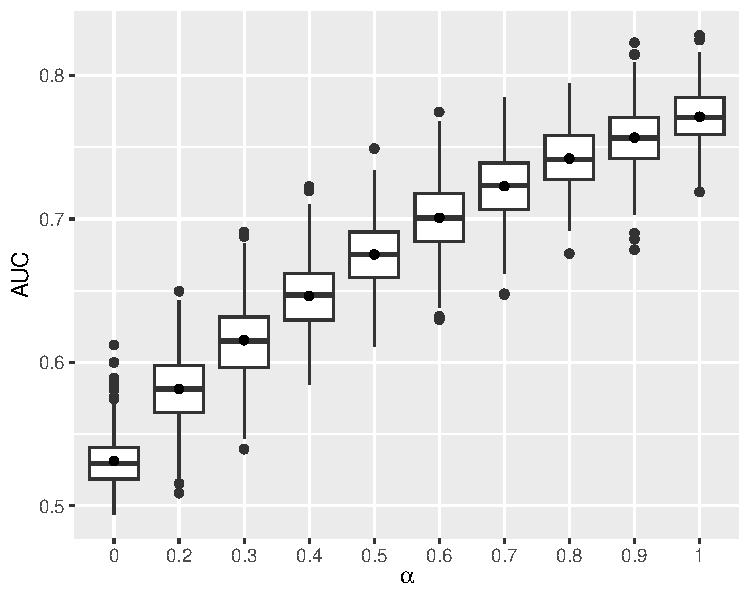
\includegraphics[width=5.5in]{../simFigs/alphaAUC.pdf}

\end{center}
%\begin{table}
%\caption{Coverage of nominal 95\% confidence intervals}
\clearpage

\subsection{Full Empirical 95\% Interval Coverage Results}
The following tables give the empirical coverage of nominal 95\% intervals for \textsc{geepers} and mixture model principal effect estimates under varying data generating models. First we show results when $n=500$ per condition, and then when $n=1000$ per condition. \\

\begin{table}
  \caption{Empirical coverage of nominal 95\% Confidence intervals for \geepers and \pmm when $n=500$ per condition.}
  
\begin{tabular}[t]{lllrlllllll}
\toprule
\multicolumn{5}{c}{ } & \multicolumn{6}{c}{$n=500$} \\
\cmidrule(l{3pt}r{3pt}){6-11}
\multicolumn{5}{c}{ } & \multicolumn{2}{c}{$\alpha=0$} & \multicolumn{2}{c}{$\alpha=0.2$} & \multicolumn{2}{c}{$\alpha=0.5$} \\
\cmidrule(l{3pt}r{3pt}){6-7} \cmidrule(l{3pt}r{3pt}){8-9} \cmidrule(l{3pt}r{3pt}){10-11}
\makecell[l]{Residual\\Dist.} & \makecell[l]{$\bm{x}:Z$\\Int.?} & \makecell[l]{$\bm{x}:S_T$\\Int.?} & $\beta_1$ & \makecell[l]{Prin.\\Eff} & \textsc{geepers} & \textsc{pmm} & \textsc{geepers} & \textsc{pmm} & \textsc{geepers} & \textsc{pmm}\\
\midrule
 & No & No & 0.0 & $\tau^0$ & 1.00 & 1.00 & 0.98 & 0.98 & 0.97 & 0.96\\

 & No & No & 0.0 & $\tau^1$ & 1.00 & 1.00 & 0.97 & 0.97 & 0.97 & 0.95\\

 & Yes & No & 0.0 & $\tau^0$ & \rd{0.84} & \rd{0.70} & \rd{0.91} & \rd{0.74} & \rd{0.93} & \rd{0.81}\\

 & Yes & No & 0.0 & $\tau^1$ & \rd{0.85} & \rd{0.70} & \rd{0.91} & \rd{0.74} & \rd{0.93} & \rd{0.82}\\

 & No & Yes & 0.0 & $\tau^0$ & \rd{1.00} & \rd{1.00} & \rd{0.98} & \rd{0.99} & \rd{0.95} & \rd{0.95}\\

 & No & Yes & 0.0 & $\tau^1$ & \rd{1.00} & \rd{0.99} & \rd{0.98} & \rd{0.99} & \rd{0.95} & \rd{0.95}\\

 & Yes & Yes & 0.0 & $\tau^0$ & \rd{0.88} & \rd{0.76} & \rd{0.91} & \rd{0.77} & \rd{0.94} & \rd{0.83}\\

\multirow{-8}{*}{\raggedright\arraybackslash Normal} & Yes & Yes & 0.0 & $\tau^1$ & \rd{0.86} & \rd{0.74} & \rd{0.92} & \rd{0.76} & \rd{0.94} & \rd{0.82}\\
\cmidrule{1-11}
 & No & No & 0.0 & $\tau^0$ & 1.00 & \rd{0.15} & 0.96 & \rd{0.24} & 0.96 & \rd{0.50}\\

 & No & No & 0.0 & $\tau^1$ & 1.00 & \rd{0.16} & 0.97 & \rd{0.23} & 0.95 & \rd{0.49}\\

 & Yes & No & 0.0 & $\tau^0$ & \rd{0.85} & \rd{0.05} & \rd{0.83} & \rd{0.09} & \rd{0.95} & \rd{0.34}\\

 & Yes & No & 0.0 & $\tau^1$ & \rd{0.85} & \rd{0.06} & \rd{0.85} & \rd{0.09} & \rd{0.93} & \rd{0.33}\\

 & No & Yes & 0.0 & $\tau^0$ & \rd{1.00} & \rd{0.27} & \rd{0.99} & \rd{0.26} & \rd{0.95} & \rd{0.50}\\

 & No & Yes & 0.0 & $\tau^1$ & \rd{1.00} & \rd{0.28} & \rd{0.98} & \rd{0.26} & \rd{0.96} & \rd{0.52}\\

 & Yes & Yes & 0.0 & $\tau^0$ & \rd{0.83} & \rd{0.11} & \rd{0.86} & \rd{0.18} & \rd{0.92} & \rd{0.45}\\

\multirow{-8}{*}{\raggedright\arraybackslash Uniform} & Yes & Yes & 0.0 & $\tau^1$ & \rd{0.81} & \rd{0.11} & \rd{0.85} & \rd{0.17} & \rd{0.92} & \rd{0.45}\\
\cmidrule{1-11}
 & No & No & 0.3 & $\tau^0$ & 0.99 & 0.99 & 0.97 & 0.98 & 0.95 & 0.96\\

 & No & No & 0.3 & $\tau^1$ & 0.99 & 0.99 & 0.97 & 0.97 & 0.96 & 0.96\\

 & Yes & No & 0.3 & $\tau^0$ & \rd{0.88} & \rd{0.75} & \rd{0.88} & \rd{0.76} & \rd{0.94} & \rd{0.89}\\

 & Yes & No & 0.3 & $\tau^1$ & \rd{0.88} & \rd{0.74} & \rd{0.88} & \rd{0.74} & \rd{0.94} & \rd{0.89}\\

 & No & Yes & 0.3 & $\tau^0$ & \rd{0.99} & \rd{0.99} & \rd{0.97} & \rd{0.96} & \rd{0.96} & \rd{0.97}\\

 & No & Yes & 0.3 & $\tau^1$ & \rd{1.00} & \rd{1.00} & \rd{0.98} & \rd{0.97} & \rd{0.97} & \rd{0.96}\\

 & Yes & Yes & 0.3 & $\tau^0$ & \rd{0.90} & \rd{0.78} & \rd{0.90} & \rd{0.76} & \rd{0.93} & \rd{0.89}\\

\multirow{-8}{*}{\raggedright\arraybackslash Normal} & Yes & Yes & 0.3 & $\tau^1$ & \rd{0.90} & \rd{0.77} & \rd{0.90} & \rd{0.77} & \rd{0.94} & \rd{0.88}\\
\cmidrule{1-11}
 & No & No & 0.3 & $\tau^0$ & 0.99 & \rd{0.29} & 0.98 & \rd{0.39} & 0.95 & \rd{0.61}\\

 & No & No & 0.3 & $\tau^1$ & 0.99 & \rd{0.29} & 0.97 & \rd{0.40} & 0.95 & \rd{0.61}\\

 & Yes & No & 0.3 & $\tau^0$ & \rd{0.83} & \rd{0.12} & \rd{0.87} & \rd{0.21} & \rd{0.94} & \rd{0.48}\\

 & Yes & No & 0.3 & $\tau^1$ & \rd{0.83} & \rd{0.11} & \rd{0.87} & \rd{0.20} & \rd{0.93} & \rd{0.48}\\

 & No & Yes & 0.3 & $\tau^0$ & \rd{1.00} & \rd{0.47} & \rd{0.97} & \rd{0.49} & \rd{0.95} & \rd{0.60}\\

 & No & Yes & 0.3 & $\tau^1$ & \rd{1.00} & \rd{0.47} & \rd{0.98} & \rd{0.53} & \rd{0.96} & \rd{0.57}\\

 & Yes & Yes & 0.3 & $\tau^0$ & \rd{0.83} & \rd{0.16} & \rd{0.89} & \rd{0.21} & \rd{0.95} & \rd{0.52}\\

\multirow{-8}{*}{\raggedright\arraybackslash Uniform} & Yes & Yes & 0.3 & $\tau^1$ & \rd{0.83} & \rd{0.15} & \rd{0.88} & \rd{0.21} & \rd{0.94} & \rd{0.53}\\
\bottomrule
\end{tabular}

 \end{table}

 \begin{table}
  \caption{Empirical coverage of nominal 95\% Confidence intervals for \geepers and \pmm when $n=1000$ per condition.}
  
\begin{tabular}[t]{lllrlllllll}
\toprule
\multicolumn{5}{c}{ } & \multicolumn{6}{c}{$n=1000$} \\
\cmidrule(l{3pt}r{3pt}){6-11}
\multicolumn{5}{c}{ } & \multicolumn{2}{c}{$\alpha=0$} & \multicolumn{2}{c}{$\alpha=0.2$} & \multicolumn{2}{c}{$\alpha=0.5$} \\
\cmidrule(l{3pt}r{3pt}){6-7} \cmidrule(l{3pt}r{3pt}){8-9} \cmidrule(l{3pt}r{3pt}){10-11}
\makecell[l]{Residual\\Dist.} & \makecell[l]{X:Z\\Int.?} & \makecell[l]{X:S\\Int.?} & $\beta_1$ & \makecell[l]{Prin.\\Eff} & \geepers & \pmm & \geepers & \pmm & \geepers & \pmm\\
\midrule
 & No & No & 0.0 & $\tau^0$ & 1.00 & 1.00 & 0.97 & 0.96 & 0.94 & 0.94\\

 & No & No & 0.0 & $\tau^1$ & 1.00 & 1.00 & 0.96 & 0.96 & 0.95 & 0.95\\

 & Yes & No & 0.0 & $\tau^0$ & \rd{0.84} & \rd{0.48} & \rd{0.87} & \rd{0.51} & \rd{0.93} & \rd{0.75}\\

 & Yes & No & 0.0 & $\tau^1$ & \rd{0.85} & \rd{0.49} & \rd{0.87} & \rd{0.49} & \rd{0.93} & \rd{0.76}\\

 & No & Yes & 0.0 & $\tau^0$ & \rd{0.99} & \rd{1.00} & \rd{0.96} & \rd{0.97} & \rd{0.95} & \rd{0.95}\\

 & No & Yes & 0.0 & $\tau^1$ & \rd{0.99} & \rd{1.00} & \rd{0.96} & \rd{0.97} & \rd{0.95} & \rd{0.95}\\

 & Yes & Yes & 0.0 & $\tau^0$ & \rd{0.86} & \rd{0.53} & \rd{0.91} & \rd{0.55} & \rd{0.94} & \rd{0.80}\\

\multirow{-8}{*}{\raggedright\arraybackslash Normal} & Yes & Yes & 0.0 & $\tau^1$ & \rd{0.85} & \rd{0.52} & \rd{0.90} & \rd{0.55} & \rd{0.93} & \rd{0.78}\\
\cmidrule{1-11}
 & No & No & 0.0 & $\tau^0$ & 1.00 & \rd{0.00} & 0.97 & \rd{0.00} & 0.95 & \rd{0.21}\\

 & No & No & 0.0 & $\tau^1$ & 1.00 & \rd{0.00} & 0.97 & \rd{0.00} & 0.95 & \rd{0.22}\\

 & Yes & No & 0.0 & $\tau^0$ & \rd{0.87} & \rd{0.00} & \rd{0.88} & \rd{0.00} & \rd{0.92} & \rd{0.08}\\

 & Yes & No & 0.0 & $\tau^1$ & \rd{0.87} & \rd{0.00} & \rd{0.88} & \rd{0.00} & \rd{0.94} & \rd{0.08}\\

 & No & Yes & 0.0 & $\tau^0$ & \rd{1.00} & \rd{0.00} & \rd{0.98} & \rd{0.01} & \rd{0.94} & \rd{0.33}\\

 & No & Yes & 0.0 & $\tau^1$ & \rd{1.00} & \rd{0.00} & \rd{0.99} & \rd{0.01} & \rd{0.95} & \rd{0.33}\\

 & Yes & Yes & 0.0 & $\tau^0$ & \rd{0.80} & \rd{0.00} & \rd{0.87} & \rd{0.00} & \rd{0.91} & \rd{0.14}\\

\multirow{-8}{*}{\raggedright\arraybackslash Uniform} & Yes & Yes & 0.0 & $\tau^1$ & \rd{0.80} & \rd{0.00} & \rd{0.89} & \rd{0.00} & \rd{0.93} & \rd{0.14}\\
\cmidrule{1-11}
 & No & No & 0.3 & $\tau^0$ & 1.00 & 1.00 & 0.96 & 0.97 & 0.94 & 0.94\\

 & No & No & 0.3 & $\tau^1$ & 1.00 & 0.99 & 0.97 & 0.97 & 0.95 & 0.96\\

 & Yes & No & 0.3 & $\tau^0$ & \rd{0.87} & \rd{0.55} & \rd{0.89} & \rd{0.60} & \rd{0.94} & \rd{0.80}\\

 & Yes & No & 0.3 & $\tau^1$ & \rd{0.87} & \rd{0.55} & \rd{0.90} & \rd{0.60} & \rd{0.93} & \rd{0.79}\\

 & No & Yes & 0.3 & $\tau^0$ & \rd{1.00} & \rd{1.00} & \rd{0.97} & \rd{0.96} & \rd{0.95} & \rd{0.97}\\

 & No & Yes & 0.3 & $\tau^1$ & \rd{1.00} & \rd{1.00} & \rd{0.97} & \rd{0.97} & \rd{0.94} & \rd{0.96}\\

 & Yes & Yes & 0.3 & $\tau^0$ & \rd{0.86} & \rd{0.55} & \rd{0.91} & \rd{0.62} & \rd{0.95} & \rd{0.83}\\

\multirow{-8}{*}{\raggedright\arraybackslash Normal} & Yes & Yes & 0.3 & $\tau^1$ & \rd{0.85} & \rd{0.54} & \rd{0.91} & \rd{0.62} & \rd{0.91} & \rd{0.81}\\
\cmidrule{1-11}
 & No & No & 0.3 & $\tau^0$ & 0.99 & \rd{0.00} & 0.95 & \rd{0.01} & 0.96 & \rd{0.31}\\

 & No & No & 0.3 & $\tau^1$ & 1.00 & \rd{0.00} & 0.95 & \rd{0.01} & 0.96 & \rd{0.30}\\

 & Yes & No & 0.3 & $\tau^0$ & \rd{0.88} & \rd{0.00} & \rd{0.91} & \rd{0.00} & \rd{0.91} & \rd{0.17}\\

 & Yes & No & 0.3 & $\tau^1$ & \rd{0.88} & \rd{0.00} & \rd{0.90} & \rd{0.00} & \rd{0.92} & \rd{0.17}\\

 & No & Yes & 0.3 & $\tau^0$ & \rd{1.00} & \rd{0.02} & \rd{0.96} & \rd{0.07} & \rd{0.97} & \rd{0.41}\\

 & No & Yes & 0.3 & $\tau^1$ & \rd{1.00} & \rd{0.02} & \rd{0.95} & \rd{0.07} & \rd{0.97} & \rd{0.40}\\

 & Yes & Yes & 0.3 & $\tau^0$ & \rd{0.87} & \rd{0.00} & \rd{0.89} & \rd{0.03} & \rd{0.95} & \rd{0.22}\\

\multirow{-8}{*}{\raggedright\arraybackslash Uniform} & Yes & Yes & 0.3 & $\tau^1$ & \rd{0.86} & \rd{0.00} & \rd{0.87} & \rd{0.03} & \rd{0.92} & \rd{0.21}\\
\bottomrule
\end{tabular}

 \end{table}


 

\clearpage
\subsection{Full RMSE Results}
The following table gives the root mean squared error (RMSE), $\left\{\sum_b (\hat{\tau}-\tau)^2/500\right\}^{1/2}$, for \textsc{geepers}, mixture model, and principal score weighting principal effect estimates under varying data generating models.\\

\begin{table}
  \caption{Empirical RMSE  for \geepers, \pmm, and \psw when $n=500$ per condition.}
  
\begin{tabular}[t]{llllrrrrrr}
\toprule
\multicolumn{4}{c}{ } & \multicolumn{6}{c}{$n=500$} \\
\cmidrule(l{3pt}r{3pt}){5-10}
\multicolumn{4}{c}{ } & \multicolumn{3}{c}{$\alpha=0.2$} & \multicolumn{3}{c}{$\alpha=0.5$} \\
\cmidrule(l{3pt}r{3pt}){5-7} \cmidrule(l{3pt}r{3pt}){8-10}
\makecell[l]{Residual\\Dist.} & \makecell[l]{$\bm{x}:Z$\\Int.?} & \makecell[l]{$\bm{x}:S_T$\\Int.?} & Parameter & \textsc{geepers} & \textsc{pmm} & \textsc{psw} & \textsc{geepers} & \textsc{pmm} & \textsc{psw}\\
\midrule
 & No & No & $\tau^0$ & 0.56 & 0.17 & 0.09 & 0.17 & 0.15 & 0.11\\

 & No & No & $\tau^1$ & 0.57 & 0.17 & 0.08 & 0.17 & 0.15 & 0.12\\

 & Yes & No & $\tau^0$ & 0.94 & 0.29 & 0.09 & 0.23 & 0.23 & 0.12\\

 & Yes & No & $\tau^1$ & 0.94 & 0.30 & 0.09 & 0.23 & 0.23 & 0.13\\

 & No & Yes & $\tau^0$ & 0.48 & 0.17 & 0.08 & 0.18 & 0.16 & 0.11\\

 & No & Yes & $\tau^1$ & 0.46 & 0.16 & 0.08 & 0.18 & 0.15 & 0.12\\

 & Yes & Yes & $\tau^0$ & 0.98 & 0.29 & 0.09 & 0.23 & 0.23 & 0.12\\

\multirow{-8}{*}{\raggedright\arraybackslash Normal} & Yes & Yes & $\tau^1$ & 0.99 & 0.29 & 0.09 & 0.23 & 0.23 & 0.12\\
\cmidrule{1-10}
 & No & No & $\tau^0$ & 0.42 & 0.55 & 0.09 & 0.18 & 0.42 & 0.11\\

 & No & No & $\tau^1$ & 0.42 & 0.54 & 0.08 & 0.18 & 0.42 & 0.12\\

 & Yes & No & $\tau^0$ & 1.58 & 0.58 & 0.09 & 0.22 & 0.46 & 0.12\\

 & Yes & No & $\tau^1$ & 1.60 & 0.57 & 0.08 & 0.22 & 0.46 & 0.12\\

 & No & Yes & $\tau^0$ & 0.41 & 0.53 & 0.09 & 0.19 & 0.41 & 0.11\\

 & No & Yes & $\tau^1$ & 0.41 & 0.54 & 0.08 & 0.19 & 0.41 & 0.12\\

 & Yes & Yes & $\tau^0$ & 2.70 & 0.55 & 0.09 & 0.23 & 0.44 & 0.12\\

\multirow{-8}{*}{\raggedright\arraybackslash Uniform} & Yes & Yes & $\tau^1$ & 2.29 & 0.57 & 0.09 & 0.24 & 0.44 & 0.13\\
\bottomrule
\end{tabular}

 \end{table}


 \begin{table}
  \caption{Empirical RMSE  for \geepers, \pmm, and \psw when $n=1000$ per condition.}
  
\begin{tabular}[t]{lllrlll}
\toprule
\multicolumn{5}{c}{ } & \multicolumn{6}{c}{$n=1000$} \\
\cmidrule(l{3pt}r{3pt}){6-11}
\multicolumn{5}{c}{ } & \multicolumn{3}{c}{$\alpha=0.2$} & \multicolumn{3}{c}{$\alpha=0.5$} \\
\cmidrule(l{3pt}r{3pt}){6-8} \cmidrule(l{3pt}r{3pt}){9-11}
\makecell[l]{Residual\\Dist.} & \makecell[l]{$\bm{x}:Z$\\Int.?} & \makecell[l]{$\bm{x}:S_T$\\Int.?} & $\beta_1$ & \makecell[l]{Prin.\\Eff} & NA & NA\\
\midrule
 & No & No & 0.0 & $\tau^0$ & 0.28614523, 0.15955541, 0.06634178 & 0.1334332, 0.1118913, 0.2301330\\

 & No & No & 0.0 & $\tau^1$ & 0.28698999, 0.16003274, 0.06642983 & 0.1312804, 0.1101555, 0.2263442\\

 & Yes & No & 0.0 & $\tau^0$ & 0.63273196, 0.33191436, 0.06793985 & 0.1602354, 0.1542353, 0.2280050\\

 & Yes & No & 0.0 & $\tau^1$ & 0.63687828, 0.33633998, 0.07082269 & 0.1660086, 0.1621297, 0.2340535\\

 & No & Yes & 0.0 & $\tau^0$ & 0.29800383, 0.15846149, 0.06277431 & 0.1337284, 0.1084597, 0.2297158\\

 & No & Yes & 0.0 & $\tau^1$ & 0.29743087, 0.15779350, 0.06785113 & 0.1343788, 0.1088816, 0.2293977\\

 & Yes & Yes & 0.0 & $\tau^0$ & 0.65217667, 0.32705412, 0.06552952 & 0.1597539, 0.1563865, 0.2315080\\

\multirow{-8}{*}{\raggedright\arraybackslash Normal} & Yes & Yes & 0.0 & $\tau^1$ & 0.66944417, 0.33455905, 0.07120576 & 0.1730754, 0.1594959, 0.2311189\\
\cmidrule{1-7}
 & No & No & 0.0 & $\tau^0$ & 0.30553664, 0.60640609, 0.06835612 & 0.1286616, 0.3204181, 0.2300569\\

 & No & No & 0.0 & $\tau^1$ & 0.30740028, 0.60569824, 0.06483881 & 0.1302221, 0.3264583, 0.2292238\\

 & Yes & No & 0.0 & $\tau^0$ & 0.61409087, 0.59784266, 0.07504119 & 0.1635624, 0.3625994, 0.2305085\\

 & Yes & No & 0.0 & $\tau^1$ & 0.61363329, 0.59955143, 0.06869204 & 0.1673316, 0.3597955, 0.2371051\\

 & No & Yes & 0.0 & $\tau^0$ & 0.26886669, 0.59409192, 0.06710054 & 0.1206525, 0.2890499, 0.2303636\\

 & No & Yes & 0.0 & $\tau^1$ & 0.26397806, 0.59693309, 0.06601589 & 0.1213490, 0.2878535, 0.2355593\\

 & Yes & Yes & 0.0 & $\tau^0$ & 0.59569881, 0.60088276, 0.06370024 & 0.1566310, 0.3441396, 0.2306057\\

\multirow{-8}{*}{\raggedright\arraybackslash Uniform} & Yes & Yes & 0.0 & $\tau^1$ & 0.60498441, 0.60193854, 0.07007712 & 0.1656667, 0.3366524, 0.2327784\\
\cmidrule{1-7}
 & No & No & 0.3 & $\tau^0$ & 0.2827230, 0.1737796, 0.1939610 & 0.1334332, 0.1118913, 0.2301330\\

 & No & No & 0.3 & $\tau^1$ & 0.2830708, 0.1712405, 0.1901653 & 0.1312804, 0.1101555, 0.2263442\\

 & Yes & No & 0.3 & $\tau^0$ & 0.6542264, 0.3440573, 0.1966910 & 0.1602354, 0.1542353, 0.2280050\\

 & Yes & No & 0.3 & $\tau^1$ & 0.6611211, 0.3508378, 0.1933766 & 0.1660086, 0.1621297, 0.2340535\\

 & No & Yes & 0.3 & $\tau^0$ & 0.2802360, 0.1810313, 0.1929841 & 0.1337284, 0.1084597, 0.2297158\\

 & No & Yes & 0.3 & $\tau^1$ & 0.2837333, 0.1831605, 0.1979786 & 0.1343788, 0.1088816, 0.2293977\\

 & Yes & Yes & 0.3 & $\tau^0$ & 0.6512733, 0.3317055, 0.1964653 & 0.1597539, 0.1563865, 0.2315080\\

\multirow{-8}{*}{\raggedright\arraybackslash Normal} & Yes & Yes & 0.3 & $\tau^1$ & 0.6570717, 0.3399707, 0.1932301 & 0.1730754, 0.1594959, 0.2311189\\
\cmidrule{1-7}
 & No & No & 0.3 & $\tau^0$ & 0.3539324, 0.5749586, 0.1917318 & 0.1286616, 0.3204181, 0.2300569\\

 & No & No & 0.3 & $\tau^1$ & 0.3555457, 0.5805273, 0.1929551 & 0.1302221, 0.3264583, 0.2292238\\

 & Yes & No & 0.3 & $\tau^0$ & 0.5915788, 0.6068832, 0.2007860 & 0.1635624, 0.3625994, 0.2305085\\

 & Yes & No & 0.3 & $\tau^1$ & 0.6047826, 0.6099683, 0.1931586 & 0.1673316, 0.3597955, 0.2371051\\

 & No & Yes & 0.3 & $\tau^0$ & 0.2763328, 0.5714127, 0.1958715 & 0.1206525, 0.2890499, 0.2303636\\

 & No & Yes & 0.3 & $\tau^1$ & 0.2704888, 0.5695698, 0.1926049 & 0.1213490, 0.2878535, 0.2355593\\

 & Yes & Yes & 0.3 & $\tau^0$ & 0.6718339, 0.5789302, 0.1904290 & 0.1566310, 0.3441396, 0.2306057\\

\multirow{-8}{*}{\raggedright\arraybackslash Uniform} & Yes & Yes & 0.3 & $\tau^1$ & 0.6902849, 0.5810495, 0.1982476 & 0.1656667, 0.3366524, 0.2327784\\
\bottomrule
\end{tabular}

 \end{table}

%\end{table}
\clearpage


\section{Additional Results from the OPT Study}
\singlespacing
\subsection{Summary Statistics}
The following table gives summary statistics for covariates and post-treatment outcomes in two of the conditions from the empirical study.\\

\begin{table}

\caption{\label{tab:optTab1}Descriptive statistics---mean and standard deviation or count and percent---for study variables in the full OPT dataset and in the analysis sample (i.e., complete cases)}
\centering
\begin{tabular}[t]{lllll}
\toprule
\multicolumn{1}{c}{ } & \multicolumn{2}{c}{Full Data} & \multicolumn{2}{c}{Complete Cases} \\
\cmidrule(l{3pt}r{3pt}){2-3} \cmidrule(l{3pt}r{3pt}){4-5}
  & Control & Treatment & Control & Treatment\\
\midrule
n & 410 & 413 & 326 & 314\\
Fibrinogen & 21.3 (14.9) & 20.2 (13.3) & 21.5 (15.4) & 20 (13.1)\\
Endotoxin & 1.8 (1.1) & 1.8 (1.1) & 1.8 (1.1) & 1.8 (1.1)\\
\% Sites Bleeding & 67.3 (21.1) & 43.9 (20.4) & 67.6 (21.3) & 43.5 (20.3)\\
Trt. Completed: No & - & 14 (3.4\%) & - & 4 (1.3\%)\\
\addlinespace
Trt. Completed: Und & - & 196 (47.5\%) & - & 153 (48.7\%)\\
Trt. Completed: Yes & - & 185 (44.8\%) & - & 157 (50\%)\\
\bottomrule
\end{tabular}
\end{table}

\section{Additional Results from the Applications}
\singlespacing
The following table gives summary statistics for covariates and post-treatment outcomes in two of the conditions from the empirical study.\\


\subsection{Summary Statistics}
The following table gives summary statistics for covariates and post-treatment outcomes in two of the conditions from the empirical study.\\
\small
% latex table generated in R 4.2.2 by xtable 1.8-4 package
% Mon Nov  6 17:52:58 2023
\begin{sidewaystable}[ht]
\centering
\begin{tabular}{llllllll}
  \hline
  &   & ASSISTments & BAU & Dragon & FH2T & Miss. \% & Imp. Err. (PFC) \\ 
  \hline
n &  &  402 &  385 &  369 &  791 &      &  \\ 
  Modality & In-Person &  260 (64.7)  &  238 (61.8)  &  241 (65.3)  &  529 (66.9)  &  0.0 & 0 \\ 
   & Remote &  142 (35.3)  &  147 (38.2)  &  128 (34.7)  &  262 (33.1)  &      &  \\ 
  Gender & Female &  206 (51.2)  &  193 (50.1)  &  178 (48.2)  &  376 (47.5)  &  0.0 & 0 \\ 
   & Male &  196 (48.8)  &  192 (49.9)  &  191 (51.8)  &  415 (52.5)  &      &  \\ 
  Race/Ethnicity & White &  213 (53.0)  &  192 (49.9)  &  182 (49.5)  &  409 (51.7)  &  0.1 & 0.28 \\ 
   & Hispanic/Latino &   56 (13.9)  &   51 (13.2)  &   67 (18.2)  &  120 (15.2)  &      &  \\ 
   & Asian &   98 (24.4)  &  106 (27.5)  &   89 (24.2)  &  198 (25.0)  &      &  \\ 
   & Other &   35 ( 8.7)  &   36 ( 9.4)  &   30 ( 8.2)  &   64 ( 8.1)  &      &  \\ 
  Grade 5 Perf. Lev. & Beginning Learner &   12 ( 3.3)  &    8 ( 2.4)  &   14 ( 4.5)  &   23 ( 3.3)  & 12.4 & 0.01 \\ 
   & Developing Learner &   64 (17.8)  &   62 (18.3)  &   53 (16.9)  &  124 (17.9)  &      &  \\ 
   & Distinguished Learner &  158 (43.9)  &  152 (45.0)  &  141 (44.9)  &  306 (44.2)  &      &  \\ 
   & Proficient Learner &  126 (35.0)  &  116 (34.3)  &  106 (33.8)  &  240 (34.6)  &      &  \\ 
  Pretest-Procedural &  & 1.70 (0.92) & 1.55 (1.01) & 1.64 (0.96) & 1.57 (0.98) &  5.0 & 0.42 \\ 
  Pretest-Flexibility &  & 1.47 (0.93) & 1.43 (0.93) & 1.51 (0.91) & 1.49 (0.92) &  5.0 & 0.4 \\ 
  Has EIP &  &  31 ( 7.7)  &  27 ( 7.0)  &  31 ( 8.4)  &  56 ( 7.1)  &  0.0 & 0 \\ 
  ESOL &  &  31 ( 7.7)  &  36 ( 9.4)  &  45 (12.2)  &  75 ( 9.5)  &  0.0 & 0 \\ 
  Gifted &  &  72 (17.9)  &  69 (17.9)  &  53 (14.4)  & 129 (16.3)  &  0.0 & 0 \\ 
  Has IEP &  &  38 ( 9.5)  &  40 (10.4)  &  41 (11.1)  &  60 ( 7.6)  &  0.0 & 0 \\ 
  IST &  &  25 ( 6.9)  &  27 ( 7.8)  &  23 ( 7.3)  &  58 ( 8.3)  & 11.6 & 0.06 \\ 
  SECTION504 &  &  14 ( 3.9)  &  10 ( 2.9)  &   7 ( 2.2)  &  14 ( 2.0)  & 11.6 & 0.03 \\ 
  SST &  &  11 ( 3.0)  &  12 ( 3.5)  &  13 ( 4.1)  &  31 ( 4.4)  & 11.6 & 0.03 \\ 
  fullYear5 &  & 337 (93.4)  & 321 (93.3)  & 298 (94.3)  & 659 (94.1)  & 11.6 & 0.06 \\ 
  fullYear6 &  & 368 (96.3)  & 353 (95.7)  & 328 (93.4)  & 728 (95.9)  &  4.4 & 0.04 \\ 
  noUnexcused5 &  & 112 (31.0)  &  98 (28.5)  &  93 (29.4)  & 200 (28.6)  & 11.6 & 0 \\ 
   \hline
Bottom-Outer &  & 191 (47.5)  &   0 ( 0.0)  &   0 ( 0.0)  &   0 ( 0.0)  &  0.0 &  \\ 
   \hline
\end{tabular}
\caption{Counts and percentages for categorical study variables, by randomized condition. Imputation error is the proportion falsly classified, as estimated using by missForest using out-of-bag observations. All variables were measured at baseline, with the exception of "Bottom-Outer," the principal stratification variable.} 
\label{table:tab1fac}
\end{sidewaystable}

\clearpage

\small
% latex table generated in R 4.2.2 by xtable 1.8-4 package
% Mon Nov  6 15:43:04 2023
\begin{sidewaystable}[ht]
\centering
\begin{tabular}{rlllll}
  \hline
 & ASSISTments & BAU & Dragon & Miss. \% & Imp. Err. (NRMSE) \\ 
  \hline
n &    402 &    385 &    369 &    791 &  \\ 
  Grade 5 Stand. Test & 575.32 (61.16) & 578.82 (59.86) & 574.24 (63.32) & 576.20 (60.99) & 784.69 \\ 
  log(Days Abs. 5th+1) &   1.49 (0.77) &   1.55 (0.78) &   1.48 (0.76) &   1.54 (0.81) & 0.29 \\ 
  log(Days Unexc. 5th+1) &   0.87 (0.72) &   0.93 (0.73) &   0.86 (0.69) &   0.93 (0.74) & 0.12 \\ 
  log(Days Abs. 6th+1) &   1.32 (0.73) &   1.29 (0.74) &   1.26 (0.71) &   1.33 (0.76) & 0.22 \\ 
  log(Days Unexc. 6th+1) &   0.80 (0.66) &   0.80 (0.64) &   0.72 (0.62) &   0.82 (0.69) & 0.2 \\ 
  Pretest &   4.89 (2.70) &   4.73 (2.70) &   4.99 (2.60) &   4.80 (2.69) & 1.02 \\ 
  Pretest-\# Completed &   9.36 (2.33) &   9.27 (2.45) &   9.18 (2.68) &   9.47 (2.13) & 0 \\ 
  log(Pretest ToT) &   6.41 (0.74) &   6.40 (0.83) &   6.45 (0.71) &   6.44 (0.76) & 0.37 \\ 
  Math Anxiety &  13.93 (5.66) &  13.72 (5.98) &  12.94 (5.71) &  13.62 (5.91) & 23.22 \\ 
  Math Self-Eff &  17.19 (4.95) &  17.44 (4.78) &  18.10 (4.55) &  17.63 (4.77) & 15.06 \\ 
  Perceptual Sens. &   7.50 (2.91) &   7.71 (2.94) &   7.44 (3.16) &   7.46 (3.00) & 0.54 \\ 
  Perc. Sens. Pt 2E &   1.37 (1.26) &   1.38 (1.24) &   1.41 (1.32) &   1.37 (1.28) & 0.47 \\ 
  Perc. Sens. Pt 2NE &   1.15 (1.08) &   1.18 (1.12) &   1.17 (1.18) &   1.07 (1.09) & 0.47 \\ 
  Perc. Sens. \#Comp. &  14.81 (3.93) &  14.54 (4.39) &  14.38 (4.62) &  14.91 (3.75) & 0 \\ 
  log(PS Resp. Time) &   5.74 (0.82) &   5.78 (0.88) &   5.76 (0.84) &   5.72 (0.84) & 0.4 \\ 
   \hline
\# Bottom-Out &  22.62 (28.65) &   1.27 (8.98) &   4.72 (9.48) &   6.54 (14.72) &  \\ 
  Posttest &   4.52 (2.88) &   4.26 (2.79) &   4.75 (2.87) &   4.54 (2.95) &  \\ 
   \hline
\end{tabular}
\caption{Means and standard deviations for numeric study variables, by randomized condition. Imputation error is the normalized root mean squared error (NRMSE), as estimated using by missForest using out-of-bag observations. All variables were measured at baseline, with the exception of "\# Bottom-Out" (the number of bottom-out hints requested) and Posttest.} 
\label{table:tab1num}
\end{sidewaystable}


\subsection{Regression Results}
Regression estimates from three principal score logit models and three outcome regressions, based on the "All Covariates" principal score model, for \textsc{geepers} estimates. Standard errors shown are nominal regression errors, not sandwich corrected. Fixed-effect estimates for school (PS-models) or classroom (outcome models) are omitted.

\small
%
  \providecommand{\huxb}[2]{\arrayrulecolor[RGB]{#1}\global\arrayrulewidth=#2pt}
  \providecommand{\huxvb}[2]{\color[RGB]{#1}\vrule width #2pt}
  \providecommand{\huxtpad}[1]{\rule{0pt}{#1}}
  \providecommand{\huxbpad}[1]{\rule[-#1]{0pt}{#1}}

\begin{table}[ht]
\begin{centerbox}
\begin{threeparttable}
 \setlength{\tabcolsep}{0pt}
\begin{tabular}{l l l l l}


\hhline{>{\huxb{0, 0, 0}{0.8}}->{\huxb{0, 0, 0}{0.8}}->{\huxb{0, 0, 0}{0.8}}->{\huxb{0, 0, 0}{0.8}}->{\huxb{0, 0, 0}{0.8}}-}
\arrayrulecolor{black}

\multicolumn{1}{!{\huxvb{0, 0, 0}{0}}c!{\huxvb{0, 0, 0}{0}}}{\huxtpad{6pt + 1em}\centering \hspace{6pt}  \hspace{6pt}\huxbpad{6pt}} &
\multicolumn{1}{c!{\huxvb{0, 0, 0}{0}}}{\huxtpad{6pt + 1em}\centering \hspace{6pt} psModel \hspace{6pt}\huxbpad{6pt}} &
\multicolumn{1}{c!{\huxvb{0, 0, 0}{0}}}{\huxtpad{6pt + 1em}\centering \hspace{6pt} BAU \hspace{6pt}\huxbpad{6pt}} &
\multicolumn{1}{c!{\huxvb{0, 0, 0}{0}}}{\huxtpad{6pt + 1em}\centering \hspace{6pt} FH2T \hspace{6pt}\huxbpad{6pt}} &
\multicolumn{1}{c!{\huxvb{0, 0, 0}{0}}}{\huxtpad{6pt + 1em}\centering \hspace{6pt} DragonBox \hspace{6pt}\huxbpad{6pt}} \tabularnewline[-0.5pt]


\hhline{>{\huxb{255, 255, 255}{0.4}}->{\huxb{0, 0, 0}{0.4}}->{\huxb{0, 0, 0}{0.4}}->{\huxb{0, 0, 0}{0.4}}->{\huxb{0, 0, 0}{0.4}}-}
\arrayrulecolor{black}

\multicolumn{1}{!{\huxvb{0, 0, 0}{0}}l!{\huxvb{0, 0, 0}{0}}}{\huxtpad{6pt + 1em}\raggedright \hspace{6pt} (Intercept) \hspace{6pt}\huxbpad{6pt}} &
\multicolumn{1}{r!{\huxvb{0, 0, 0}{0}}}{\huxtpad{6pt + 1em}\raggedleft \hspace{6pt} -2.143\hphantom{0}\hphantom{0}\hphantom{0}\hphantom{0} \hspace{6pt}\huxbpad{6pt}} &
\multicolumn{1}{r!{\huxvb{0, 0, 0}{0}}}{\huxtpad{6pt + 1em}\raggedleft \hspace{6pt} 1.732\hphantom{0}\hphantom{0}\hphantom{0} \hspace{6pt}\huxbpad{6pt}} &
\multicolumn{1}{r!{\huxvb{0, 0, 0}{0}}}{\huxtpad{6pt + 1em}\raggedleft \hspace{6pt} 2.834 *** \hspace{6pt}\huxbpad{6pt}} &
\multicolumn{1}{r!{\huxvb{0, 0, 0}{0}}}{\huxtpad{6pt + 1em}\raggedleft \hspace{6pt} 2.510 **\hphantom{0} \hspace{6pt}\huxbpad{6pt}} \tabularnewline[-0.5pt]


\hhline{}
\arrayrulecolor{black}

\multicolumn{1}{!{\huxvb{0, 0, 0}{0}}l!{\huxvb{0, 0, 0}{0}}}{\huxtpad{6pt + 1em}\raggedright \hspace{6pt}  \hspace{6pt}\huxbpad{6pt}} &
\multicolumn{1}{r!{\huxvb{0, 0, 0}{0}}}{\huxtpad{6pt + 1em}\raggedleft \hspace{6pt} (1.257)\hphantom{0}\hphantom{0}\hphantom{0} \hspace{6pt}\huxbpad{6pt}} &
\multicolumn{1}{r!{\huxvb{0, 0, 0}{0}}}{\huxtpad{6pt + 1em}\raggedleft \hspace{6pt} (0.916)\hphantom{0}\hphantom{0} \hspace{6pt}\huxbpad{6pt}} &
\multicolumn{1}{r!{\huxvb{0, 0, 0}{0}}}{\huxtpad{6pt + 1em}\raggedleft \hspace{6pt} (0.718)\hphantom{0}\hphantom{0}\hphantom{0} \hspace{6pt}\huxbpad{6pt}} &
\multicolumn{1}{r!{\huxvb{0, 0, 0}{0}}}{\huxtpad{6pt + 1em}\raggedleft \hspace{6pt} (0.919)\hphantom{0}\hphantom{0}\hphantom{0} \hspace{6pt}\huxbpad{6pt}} \tabularnewline[-0.5pt]


\hhline{}
\arrayrulecolor{black}

\multicolumn{1}{!{\huxvb{0, 0, 0}{0}}l!{\huxvb{0, 0, 0}{0}}}{\huxtpad{6pt + 1em}\raggedright \hspace{6pt} Scale.Score5 \hspace{6pt}\huxbpad{6pt}} &
\multicolumn{1}{r!{\huxvb{0, 0, 0}{0}}}{\huxtpad{6pt + 1em}\raggedleft \hspace{6pt} -0.594 **\hphantom{0} \hspace{6pt}\huxbpad{6pt}} &
\multicolumn{1}{r!{\huxvb{0, 0, 0}{0}}}{\huxtpad{6pt + 1em}\raggedleft \hspace{6pt} 0.207\hphantom{0}\hphantom{0}\hphantom{0} \hspace{6pt}\huxbpad{6pt}} &
\multicolumn{1}{r!{\huxvb{0, 0, 0}{0}}}{\huxtpad{6pt + 1em}\raggedleft \hspace{6pt} 0.453 *** \hspace{6pt}\huxbpad{6pt}} &
\multicolumn{1}{r!{\huxvb{0, 0, 0}{0}}}{\huxtpad{6pt + 1em}\raggedleft \hspace{6pt} 0.049\hphantom{0}\hphantom{0}\hphantom{0}\hphantom{0} \hspace{6pt}\huxbpad{6pt}} \tabularnewline[-0.5pt]


\hhline{}
\arrayrulecolor{black}

\multicolumn{1}{!{\huxvb{0, 0, 0}{0}}l!{\huxvb{0, 0, 0}{0}}}{\huxtpad{6pt + 1em}\raggedright \hspace{6pt}  \hspace{6pt}\huxbpad{6pt}} &
\multicolumn{1}{r!{\huxvb{0, 0, 0}{0}}}{\huxtpad{6pt + 1em}\raggedleft \hspace{6pt} (0.188)\hphantom{0}\hphantom{0}\hphantom{0} \hspace{6pt}\huxbpad{6pt}} &
\multicolumn{1}{r!{\huxvb{0, 0, 0}{0}}}{\huxtpad{6pt + 1em}\raggedleft \hspace{6pt} (0.126)\hphantom{0}\hphantom{0} \hspace{6pt}\huxbpad{6pt}} &
\multicolumn{1}{r!{\huxvb{0, 0, 0}{0}}}{\huxtpad{6pt + 1em}\raggedleft \hspace{6pt} (0.104)\hphantom{0}\hphantom{0}\hphantom{0} \hspace{6pt}\huxbpad{6pt}} &
\multicolumn{1}{r!{\huxvb{0, 0, 0}{0}}}{\huxtpad{6pt + 1em}\raggedleft \hspace{6pt} (0.132)\hphantom{0}\hphantom{0}\hphantom{0} \hspace{6pt}\huxbpad{6pt}} \tabularnewline[-0.5pt]


\hhline{}
\arrayrulecolor{black}

\multicolumn{1}{!{\huxvb{0, 0, 0}{0}}l!{\huxvb{0, 0, 0}{0}}}{\huxtpad{6pt + 1em}\raggedright \hspace{6pt} ESOL1 \hspace{6pt}\huxbpad{6pt}} &
\multicolumn{1}{r!{\huxvb{0, 0, 0}{0}}}{\huxtpad{6pt + 1em}\raggedleft \hspace{6pt} -0.825\hphantom{0}\hphantom{0}\hphantom{0}\hphantom{0} \hspace{6pt}\huxbpad{6pt}} &
\multicolumn{1}{r!{\huxvb{0, 0, 0}{0}}}{\huxtpad{6pt + 1em}\raggedleft \hspace{6pt} 0.091\hphantom{0}\hphantom{0}\hphantom{0} \hspace{6pt}\huxbpad{6pt}} &
\multicolumn{1}{r!{\huxvb{0, 0, 0}{0}}}{\huxtpad{6pt + 1em}\raggedleft \hspace{6pt} -0.459\hphantom{0}\hphantom{0}\hphantom{0}\hphantom{0} \hspace{6pt}\huxbpad{6pt}} &
\multicolumn{1}{r!{\huxvb{0, 0, 0}{0}}}{\huxtpad{6pt + 1em}\raggedleft \hspace{6pt} -0.493\hphantom{0}\hphantom{0}\hphantom{0}\hphantom{0} \hspace{6pt}\huxbpad{6pt}} \tabularnewline[-0.5pt]


\hhline{}
\arrayrulecolor{black}

\multicolumn{1}{!{\huxvb{0, 0, 0}{0}}l!{\huxvb{0, 0, 0}{0}}}{\huxtpad{6pt + 1em}\raggedright \hspace{6pt}  \hspace{6pt}\huxbpad{6pt}} &
\multicolumn{1}{r!{\huxvb{0, 0, 0}{0}}}{\huxtpad{6pt + 1em}\raggedleft \hspace{6pt} (0.642)\hphantom{0}\hphantom{0}\hphantom{0} \hspace{6pt}\huxbpad{6pt}} &
\multicolumn{1}{r!{\huxvb{0, 0, 0}{0}}}{\huxtpad{6pt + 1em}\raggedleft \hspace{6pt} (0.364)\hphantom{0}\hphantom{0} \hspace{6pt}\huxbpad{6pt}} &
\multicolumn{1}{r!{\huxvb{0, 0, 0}{0}}}{\huxtpad{6pt + 1em}\raggedleft \hspace{6pt} (0.268)\hphantom{0}\hphantom{0}\hphantom{0} \hspace{6pt}\huxbpad{6pt}} &
\multicolumn{1}{r!{\huxvb{0, 0, 0}{0}}}{\huxtpad{6pt + 1em}\raggedleft \hspace{6pt} (0.351)\hphantom{0}\hphantom{0}\hphantom{0} \hspace{6pt}\huxbpad{6pt}} \tabularnewline[-0.5pt]


\hhline{}
\arrayrulecolor{black}

\multicolumn{1}{!{\huxvb{0, 0, 0}{0}}l!{\huxvb{0, 0, 0}{0}}}{\huxtpad{6pt + 1em}\raggedright \hspace{6pt} IEP1 \hspace{6pt}\huxbpad{6pt}} &
\multicolumn{1}{r!{\huxvb{0, 0, 0}{0}}}{\huxtpad{6pt + 1em}\raggedleft \hspace{6pt} -1.335 **\hphantom{0} \hspace{6pt}\huxbpad{6pt}} &
\multicolumn{1}{r!{\huxvb{0, 0, 0}{0}}}{\huxtpad{6pt + 1em}\raggedleft \hspace{6pt} 0.148\hphantom{0}\hphantom{0}\hphantom{0} \hspace{6pt}\huxbpad{6pt}} &
\multicolumn{1}{r!{\huxvb{0, 0, 0}{0}}}{\huxtpad{6pt + 1em}\raggedleft \hspace{6pt} 0.234\hphantom{0}\hphantom{0}\hphantom{0}\hphantom{0} \hspace{6pt}\huxbpad{6pt}} &
\multicolumn{1}{r!{\huxvb{0, 0, 0}{0}}}{\huxtpad{6pt + 1em}\raggedleft \hspace{6pt} 0.096\hphantom{0}\hphantom{0}\hphantom{0}\hphantom{0} \hspace{6pt}\huxbpad{6pt}} \tabularnewline[-0.5pt]


\hhline{}
\arrayrulecolor{black}

\multicolumn{1}{!{\huxvb{0, 0, 0}{0}}l!{\huxvb{0, 0, 0}{0}}}{\huxtpad{6pt + 1em}\raggedright \hspace{6pt}  \hspace{6pt}\huxbpad{6pt}} &
\multicolumn{1}{r!{\huxvb{0, 0, 0}{0}}}{\huxtpad{6pt + 1em}\raggedleft \hspace{6pt} (0.463)\hphantom{0}\hphantom{0}\hphantom{0} \hspace{6pt}\huxbpad{6pt}} &
\multicolumn{1}{r!{\huxvb{0, 0, 0}{0}}}{\huxtpad{6pt + 1em}\raggedleft \hspace{6pt} (0.288)\hphantom{0}\hphantom{0} \hspace{6pt}\huxbpad{6pt}} &
\multicolumn{1}{r!{\huxvb{0, 0, 0}{0}}}{\huxtpad{6pt + 1em}\raggedleft \hspace{6pt} (0.255)\hphantom{0}\hphantom{0}\hphantom{0} \hspace{6pt}\huxbpad{6pt}} &
\multicolumn{1}{r!{\huxvb{0, 0, 0}{0}}}{\huxtpad{6pt + 1em}\raggedleft \hspace{6pt} (0.277)\hphantom{0}\hphantom{0}\hphantom{0} \hspace{6pt}\huxbpad{6pt}} \tabularnewline[-0.5pt]


\hhline{}
\arrayrulecolor{black}

\multicolumn{1}{!{\huxvb{0, 0, 0}{0}}l!{\huxvb{0, 0, 0}{0}}}{\huxtpad{6pt + 1em}\raggedright \hspace{6pt} pre.total\_time\_on\_tasks \hspace{6pt}\huxbpad{6pt}} &
\multicolumn{1}{r!{\huxvb{0, 0, 0}{0}}}{\huxtpad{6pt + 1em}\raggedleft \hspace{6pt} -0.447 **\hphantom{0} \hspace{6pt}\huxbpad{6pt}} &
\multicolumn{1}{r!{\huxvb{0, 0, 0}{0}}}{\huxtpad{6pt + 1em}\raggedleft \hspace{6pt} -0.131\hphantom{0}\hphantom{0}\hphantom{0} \hspace{6pt}\huxbpad{6pt}} &
\multicolumn{1}{r!{\huxvb{0, 0, 0}{0}}}{\huxtpad{6pt + 1em}\raggedleft \hspace{6pt} 0.078\hphantom{0}\hphantom{0}\hphantom{0}\hphantom{0} \hspace{6pt}\huxbpad{6pt}} &
\multicolumn{1}{r!{\huxvb{0, 0, 0}{0}}}{\huxtpad{6pt + 1em}\raggedleft \hspace{6pt} -0.003\hphantom{0}\hphantom{0}\hphantom{0}\hphantom{0} \hspace{6pt}\huxbpad{6pt}} \tabularnewline[-0.5pt]


\hhline{}
\arrayrulecolor{black}

\multicolumn{1}{!{\huxvb{0, 0, 0}{0}}l!{\huxvb{0, 0, 0}{0}}}{\huxtpad{6pt + 1em}\raggedright \hspace{6pt}  \hspace{6pt}\huxbpad{6pt}} &
\multicolumn{1}{r!{\huxvb{0, 0, 0}{0}}}{\huxtpad{6pt + 1em}\raggedleft \hspace{6pt} (0.152)\hphantom{0}\hphantom{0}\hphantom{0} \hspace{6pt}\huxbpad{6pt}} &
\multicolumn{1}{r!{\huxvb{0, 0, 0}{0}}}{\huxtpad{6pt + 1em}\raggedleft \hspace{6pt} (0.091)\hphantom{0}\hphantom{0} \hspace{6pt}\huxbpad{6pt}} &
\multicolumn{1}{r!{\huxvb{0, 0, 0}{0}}}{\huxtpad{6pt + 1em}\raggedleft \hspace{6pt} (0.073)\hphantom{0}\hphantom{0}\hphantom{0} \hspace{6pt}\huxbpad{6pt}} &
\multicolumn{1}{r!{\huxvb{0, 0, 0}{0}}}{\huxtpad{6pt + 1em}\raggedleft \hspace{6pt} (0.096)\hphantom{0}\hphantom{0}\hphantom{0} \hspace{6pt}\huxbpad{6pt}} \tabularnewline[-0.5pt]


\hhline{}
\arrayrulecolor{black}

\multicolumn{1}{!{\huxvb{0, 0, 0}{0}}l!{\huxvb{0, 0, 0}{0}}}{\huxtpad{6pt + 1em}\raggedright \hspace{6pt} pre\_MSE\_total\_score \hspace{6pt}\huxbpad{6pt}} &
\multicolumn{1}{r!{\huxvb{0, 0, 0}{0}}}{\huxtpad{6pt + 1em}\raggedleft \hspace{6pt} -0.179\hphantom{0}\hphantom{0}\hphantom{0}\hphantom{0} \hspace{6pt}\huxbpad{6pt}} &
\multicolumn{1}{r!{\huxvb{0, 0, 0}{0}}}{\huxtpad{6pt + 1em}\raggedleft \hspace{6pt} 0.201 *\hphantom{0} \hspace{6pt}\huxbpad{6pt}} &
\multicolumn{1}{r!{\huxvb{0, 0, 0}{0}}}{\huxtpad{6pt + 1em}\raggedleft \hspace{6pt} 0.120\hphantom{0}\hphantom{0}\hphantom{0}\hphantom{0} \hspace{6pt}\huxbpad{6pt}} &
\multicolumn{1}{r!{\huxvb{0, 0, 0}{0}}}{\huxtpad{6pt + 1em}\raggedleft \hspace{6pt} 0.350 *** \hspace{6pt}\huxbpad{6pt}} \tabularnewline[-0.5pt]


\hhline{}
\arrayrulecolor{black}

\multicolumn{1}{!{\huxvb{0, 0, 0}{0}}l!{\huxvb{0, 0, 0}{0}}}{\huxtpad{6pt + 1em}\raggedright \hspace{6pt}  \hspace{6pt}\huxbpad{6pt}} &
\multicolumn{1}{r!{\huxvb{0, 0, 0}{0}}}{\huxtpad{6pt + 1em}\raggedleft \hspace{6pt} (0.130)\hphantom{0}\hphantom{0}\hphantom{0} \hspace{6pt}\huxbpad{6pt}} &
\multicolumn{1}{r!{\huxvb{0, 0, 0}{0}}}{\huxtpad{6pt + 1em}\raggedleft \hspace{6pt} (0.082)\hphantom{0}\hphantom{0} \hspace{6pt}\huxbpad{6pt}} &
\multicolumn{1}{r!{\huxvb{0, 0, 0}{0}}}{\huxtpad{6pt + 1em}\raggedleft \hspace{6pt} (0.068)\hphantom{0}\hphantom{0}\hphantom{0} \hspace{6pt}\huxbpad{6pt}} &
\multicolumn{1}{r!{\huxvb{0, 0, 0}{0}}}{\huxtpad{6pt + 1em}\raggedleft \hspace{6pt} (0.084)\hphantom{0}\hphantom{0}\hphantom{0} \hspace{6pt}\huxbpad{6pt}} \tabularnewline[-0.5pt]


\hhline{}
\arrayrulecolor{black}

\multicolumn{1}{!{\huxvb{0, 0, 0}{0}}l!{\huxvb{0, 0, 0}{0}}}{\huxtpad{6pt + 1em}\raggedright \hspace{6pt} fullYear5TRUE \hspace{6pt}\huxbpad{6pt}} &
\multicolumn{1}{r!{\huxvb{0, 0, 0}{0}}}{\huxtpad{6pt + 1em}\raggedleft \hspace{6pt} 1.405 *\hphantom{0}\hphantom{0} \hspace{6pt}\huxbpad{6pt}} &
\multicolumn{1}{r!{\huxvb{0, 0, 0}{0}}}{\huxtpad{6pt + 1em}\raggedleft \hspace{6pt} -0.129\hphantom{0}\hphantom{0}\hphantom{0} \hspace{6pt}\huxbpad{6pt}} &
\multicolumn{1}{r!{\huxvb{0, 0, 0}{0}}}{\huxtpad{6pt + 1em}\raggedleft \hspace{6pt} -0.099\hphantom{0}\hphantom{0}\hphantom{0}\hphantom{0} \hspace{6pt}\huxbpad{6pt}} &
\multicolumn{1}{r!{\huxvb{0, 0, 0}{0}}}{\huxtpad{6pt + 1em}\raggedleft \hspace{6pt} 0.062\hphantom{0}\hphantom{0}\hphantom{0}\hphantom{0} \hspace{6pt}\huxbpad{6pt}} \tabularnewline[-0.5pt]


\hhline{}
\arrayrulecolor{black}

\multicolumn{1}{!{\huxvb{0, 0, 0}{0}}l!{\huxvb{0, 0, 0}{0}}}{\huxtpad{6pt + 1em}\raggedright \hspace{6pt}  \hspace{6pt}\huxbpad{6pt}} &
\multicolumn{1}{r!{\huxvb{0, 0, 0}{0}}}{\huxtpad{6pt + 1em}\raggedleft \hspace{6pt} (0.585)\hphantom{0}\hphantom{0}\hphantom{0} \hspace{6pt}\huxbpad{6pt}} &
\multicolumn{1}{r!{\huxvb{0, 0, 0}{0}}}{\huxtpad{6pt + 1em}\raggedleft \hspace{6pt} (0.328)\hphantom{0}\hphantom{0} \hspace{6pt}\huxbpad{6pt}} &
\multicolumn{1}{r!{\huxvb{0, 0, 0}{0}}}{\huxtpad{6pt + 1em}\raggedleft \hspace{6pt} (0.286)\hphantom{0}\hphantom{0}\hphantom{0} \hspace{6pt}\huxbpad{6pt}} &
\multicolumn{1}{r!{\huxvb{0, 0, 0}{0}}}{\huxtpad{6pt + 1em}\raggedleft \hspace{6pt} (0.341)\hphantom{0}\hphantom{0}\hphantom{0} \hspace{6pt}\huxbpad{6pt}} \tabularnewline[-0.5pt]


\hhline{}
\arrayrulecolor{black}

\multicolumn{1}{!{\huxvb{0, 0, 0}{0}}l!{\huxvb{0, 0, 0}{0}}}{\huxtpad{6pt + 1em}\raggedright \hspace{6pt} pre\_MA\_total\_scoreNATRUE \hspace{6pt}\huxbpad{6pt}} &
\multicolumn{1}{r!{\huxvb{0, 0, 0}{0}}}{\huxtpad{6pt + 1em}\raggedleft \hspace{6pt} -3.205 *** \hspace{6pt}\huxbpad{6pt}} &
\multicolumn{1}{r!{\huxvb{0, 0, 0}{0}}}{\huxtpad{6pt + 1em}\raggedleft \hspace{6pt} \hphantom{0}\hphantom{0}\hphantom{0}\hphantom{0}\hphantom{0}\hphantom{0}\hphantom{0} \hspace{6pt}\huxbpad{6pt}} &
\multicolumn{1}{r!{\huxvb{0, 0, 0}{0}}}{\huxtpad{6pt + 1em}\raggedleft \hspace{6pt} \hphantom{0}\hphantom{0}\hphantom{0}\hphantom{0}\hphantom{0}\hphantom{0}\hphantom{0}\hphantom{0} \hspace{6pt}\huxbpad{6pt}} &
\multicolumn{1}{r!{\huxvb{0, 0, 0}{0}}}{\huxtpad{6pt + 1em}\raggedleft \hspace{6pt} \hphantom{0}\hphantom{0}\hphantom{0}\hphantom{0}\hphantom{0}\hphantom{0}\hphantom{0}\hphantom{0} \hspace{6pt}\huxbpad{6pt}} \tabularnewline[-0.5pt]


\hhline{}
\arrayrulecolor{black}

\multicolumn{1}{!{\huxvb{0, 0, 0}{0}}l!{\huxvb{0, 0, 0}{0}}}{\huxtpad{6pt + 1em}\raggedright \hspace{6pt}  \hspace{6pt}\huxbpad{6pt}} &
\multicolumn{1}{r!{\huxvb{0, 0, 0}{0}}}{\huxtpad{6pt + 1em}\raggedleft \hspace{6pt} (0.706)\hphantom{0}\hphantom{0}\hphantom{0} \hspace{6pt}\huxbpad{6pt}} &
\multicolumn{1}{r!{\huxvb{0, 0, 0}{0}}}{\huxtpad{6pt + 1em}\raggedleft \hspace{6pt} \hphantom{0}\hphantom{0}\hphantom{0}\hphantom{0}\hphantom{0}\hphantom{0}\hphantom{0} \hspace{6pt}\huxbpad{6pt}} &
\multicolumn{1}{r!{\huxvb{0, 0, 0}{0}}}{\huxtpad{6pt + 1em}\raggedleft \hspace{6pt} \hphantom{0}\hphantom{0}\hphantom{0}\hphantom{0}\hphantom{0}\hphantom{0}\hphantom{0}\hphantom{0} \hspace{6pt}\huxbpad{6pt}} &
\multicolumn{1}{r!{\huxvb{0, 0, 0}{0}}}{\huxtpad{6pt + 1em}\raggedleft \hspace{6pt} \hphantom{0}\hphantom{0}\hphantom{0}\hphantom{0}\hphantom{0}\hphantom{0}\hphantom{0}\hphantom{0} \hspace{6pt}\huxbpad{6pt}} \tabularnewline[-0.5pt]


\hhline{}
\arrayrulecolor{black}

\multicolumn{1}{!{\huxvb{0, 0, 0}{0}}l!{\huxvb{0, 0, 0}{0}}}{\huxtpad{6pt + 1em}\raggedright \hspace{6pt} GenderM \hspace{6pt}\huxbpad{6pt}} &
\multicolumn{1}{r!{\huxvb{0, 0, 0}{0}}}{\huxtpad{6pt + 1em}\raggedleft \hspace{6pt} 0.169\hphantom{0}\hphantom{0}\hphantom{0}\hphantom{0} \hspace{6pt}\huxbpad{6pt}} &
\multicolumn{1}{r!{\huxvb{0, 0, 0}{0}}}{\huxtpad{6pt + 1em}\raggedleft \hspace{6pt} -0.186\hphantom{0}\hphantom{0}\hphantom{0} \hspace{6pt}\huxbpad{6pt}} &
\multicolumn{1}{r!{\huxvb{0, 0, 0}{0}}}{\huxtpad{6pt + 1em}\raggedleft \hspace{6pt} -0.337 **\hphantom{0} \hspace{6pt}\huxbpad{6pt}} &
\multicolumn{1}{r!{\huxvb{0, 0, 0}{0}}}{\huxtpad{6pt + 1em}\raggedleft \hspace{6pt} -0.267\hphantom{0}\hphantom{0}\hphantom{0}\hphantom{0} \hspace{6pt}\huxbpad{6pt}} \tabularnewline[-0.5pt]


\hhline{}
\arrayrulecolor{black}

\multicolumn{1}{!{\huxvb{0, 0, 0}{0}}l!{\huxvb{0, 0, 0}{0}}}{\huxtpad{6pt + 1em}\raggedright \hspace{6pt}  \hspace{6pt}\huxbpad{6pt}} &
\multicolumn{1}{r!{\huxvb{0, 0, 0}{0}}}{\huxtpad{6pt + 1em}\raggedleft \hspace{6pt} (0.253)\hphantom{0}\hphantom{0}\hphantom{0} \hspace{6pt}\huxbpad{6pt}} &
\multicolumn{1}{r!{\huxvb{0, 0, 0}{0}}}{\huxtpad{6pt + 1em}\raggedleft \hspace{6pt} (0.155)\hphantom{0}\hphantom{0} \hspace{6pt}\huxbpad{6pt}} &
\multicolumn{1}{r!{\huxvb{0, 0, 0}{0}}}{\huxtpad{6pt + 1em}\raggedleft \hspace{6pt} (0.125)\hphantom{0}\hphantom{0}\hphantom{0} \hspace{6pt}\huxbpad{6pt}} &
\multicolumn{1}{r!{\huxvb{0, 0, 0}{0}}}{\huxtpad{6pt + 1em}\raggedleft \hspace{6pt} (0.155)\hphantom{0}\hphantom{0}\hphantom{0} \hspace{6pt}\huxbpad{6pt}} \tabularnewline[-0.5pt]


\hhline{}
\arrayrulecolor{black}

\multicolumn{1}{!{\huxvb{0, 0, 0}{0}}l!{\huxvb{0, 0, 0}{0}}}{\huxtpad{6pt + 1em}\raggedright \hspace{6pt} raceEthHispanic/Latino \hspace{6pt}\huxbpad{6pt}} &
\multicolumn{1}{r!{\huxvb{0, 0, 0}{0}}}{\huxtpad{6pt + 1em}\raggedleft \hspace{6pt} -0.561\hphantom{0}\hphantom{0}\hphantom{0}\hphantom{0} \hspace{6pt}\huxbpad{6pt}} &
\multicolumn{1}{r!{\huxvb{0, 0, 0}{0}}}{\huxtpad{6pt + 1em}\raggedleft \hspace{6pt} 0.275\hphantom{0}\hphantom{0}\hphantom{0} \hspace{6pt}\huxbpad{6pt}} &
\multicolumn{1}{r!{\huxvb{0, 0, 0}{0}}}{\huxtpad{6pt + 1em}\raggedleft \hspace{6pt} 0.327\hphantom{0}\hphantom{0}\hphantom{0}\hphantom{0} \hspace{6pt}\huxbpad{6pt}} &
\multicolumn{1}{r!{\huxvb{0, 0, 0}{0}}}{\huxtpad{6pt + 1em}\raggedleft \hspace{6pt} 0.225\hphantom{0}\hphantom{0}\hphantom{0}\hphantom{0} \hspace{6pt}\huxbpad{6pt}} \tabularnewline[-0.5pt]


\hhline{}
\arrayrulecolor{black}

\multicolumn{1}{!{\huxvb{0, 0, 0}{0}}l!{\huxvb{0, 0, 0}{0}}}{\huxtpad{6pt + 1em}\raggedright \hspace{6pt}  \hspace{6pt}\huxbpad{6pt}} &
\multicolumn{1}{r!{\huxvb{0, 0, 0}{0}}}{\huxtpad{6pt + 1em}\raggedleft \hspace{6pt} (0.460)\hphantom{0}\hphantom{0}\hphantom{0} \hspace{6pt}\huxbpad{6pt}} &
\multicolumn{1}{r!{\huxvb{0, 0, 0}{0}}}{\huxtpad{6pt + 1em}\raggedleft \hspace{6pt} (0.290)\hphantom{0}\hphantom{0} \hspace{6pt}\huxbpad{6pt}} &
\multicolumn{1}{r!{\huxvb{0, 0, 0}{0}}}{\huxtpad{6pt + 1em}\raggedleft \hspace{6pt} (0.213)\hphantom{0}\hphantom{0}\hphantom{0} \hspace{6pt}\huxbpad{6pt}} &
\multicolumn{1}{r!{\huxvb{0, 0, 0}{0}}}{\huxtpad{6pt + 1em}\raggedleft \hspace{6pt} (0.283)\hphantom{0}\hphantom{0}\hphantom{0} \hspace{6pt}\huxbpad{6pt}} \tabularnewline[-0.5pt]


\hhline{}
\arrayrulecolor{black}

\multicolumn{1}{!{\huxvb{0, 0, 0}{0}}l!{\huxvb{0, 0, 0}{0}}}{\huxtpad{6pt + 1em}\raggedright \hspace{6pt} raceEthAsian \hspace{6pt}\huxbpad{6pt}} &
\multicolumn{1}{r!{\huxvb{0, 0, 0}{0}}}{\huxtpad{6pt + 1em}\raggedleft \hspace{6pt} -0.431\hphantom{0}\hphantom{0}\hphantom{0}\hphantom{0} \hspace{6pt}\huxbpad{6pt}} &
\multicolumn{1}{r!{\huxvb{0, 0, 0}{0}}}{\huxtpad{6pt + 1em}\raggedleft \hspace{6pt} 0.662 *\hphantom{0} \hspace{6pt}\huxbpad{6pt}} &
\multicolumn{1}{r!{\huxvb{0, 0, 0}{0}}}{\huxtpad{6pt + 1em}\raggedleft \hspace{6pt} 0.619 **\hphantom{0} \hspace{6pt}\huxbpad{6pt}} &
\multicolumn{1}{r!{\huxvb{0, 0, 0}{0}}}{\huxtpad{6pt + 1em}\raggedleft \hspace{6pt} 0.823 **\hphantom{0} \hspace{6pt}\huxbpad{6pt}} \tabularnewline[-0.5pt]


\hhline{}
\arrayrulecolor{black}

\multicolumn{1}{!{\huxvb{0, 0, 0}{0}}l!{\huxvb{0, 0, 0}{0}}}{\huxtpad{6pt + 1em}\raggedright \hspace{6pt}  \hspace{6pt}\huxbpad{6pt}} &
\multicolumn{1}{r!{\huxvb{0, 0, 0}{0}}}{\huxtpad{6pt + 1em}\raggedleft \hspace{6pt} (0.416)\hphantom{0}\hphantom{0}\hphantom{0} \hspace{6pt}\huxbpad{6pt}} &
\multicolumn{1}{r!{\huxvb{0, 0, 0}{0}}}{\huxtpad{6pt + 1em}\raggedleft \hspace{6pt} (0.279)\hphantom{0}\hphantom{0} \hspace{6pt}\huxbpad{6pt}} &
\multicolumn{1}{r!{\huxvb{0, 0, 0}{0}}}{\huxtpad{6pt + 1em}\raggedleft \hspace{6pt} (0.225)\hphantom{0}\hphantom{0}\hphantom{0} \hspace{6pt}\huxbpad{6pt}} &
\multicolumn{1}{r!{\huxvb{0, 0, 0}{0}}}{\huxtpad{6pt + 1em}\raggedleft \hspace{6pt} (0.298)\hphantom{0}\hphantom{0}\hphantom{0} \hspace{6pt}\huxbpad{6pt}} \tabularnewline[-0.5pt]


\hhline{}
\arrayrulecolor{black}

\multicolumn{1}{!{\huxvb{0, 0, 0}{0}}l!{\huxvb{0, 0, 0}{0}}}{\huxtpad{6pt + 1em}\raggedright \hspace{6pt} raceEthOther \hspace{6pt}\huxbpad{6pt}} &
\multicolumn{1}{r!{\huxvb{0, 0, 0}{0}}}{\huxtpad{6pt + 1em}\raggedleft \hspace{6pt} -0.131\hphantom{0}\hphantom{0}\hphantom{0}\hphantom{0} \hspace{6pt}\huxbpad{6pt}} &
\multicolumn{1}{r!{\huxvb{0, 0, 0}{0}}}{\huxtpad{6pt + 1em}\raggedleft \hspace{6pt} 0.455\hphantom{0}\hphantom{0}\hphantom{0} \hspace{6pt}\huxbpad{6pt}} &
\multicolumn{1}{r!{\huxvb{0, 0, 0}{0}}}{\huxtpad{6pt + 1em}\raggedleft \hspace{6pt} 0.208\hphantom{0}\hphantom{0}\hphantom{0}\hphantom{0} \hspace{6pt}\huxbpad{6pt}} &
\multicolumn{1}{r!{\huxvb{0, 0, 0}{0}}}{\huxtpad{6pt + 1em}\raggedleft \hspace{6pt} 0.095\hphantom{0}\hphantom{0}\hphantom{0}\hphantom{0} \hspace{6pt}\huxbpad{6pt}} \tabularnewline[-0.5pt]


\hhline{}
\arrayrulecolor{black}

\multicolumn{1}{!{\huxvb{0, 0, 0}{0}}l!{\huxvb{0, 0, 0}{0}}}{\huxtpad{6pt + 1em}\raggedright \hspace{6pt}  \hspace{6pt}\huxbpad{6pt}} &
\multicolumn{1}{r!{\huxvb{0, 0, 0}{0}}}{\huxtpad{6pt + 1em}\raggedleft \hspace{6pt} (0.492)\hphantom{0}\hphantom{0}\hphantom{0} \hspace{6pt}\huxbpad{6pt}} &
\multicolumn{1}{r!{\huxvb{0, 0, 0}{0}}}{\huxtpad{6pt + 1em}\raggedleft \hspace{6pt} (0.292)\hphantom{0}\hphantom{0} \hspace{6pt}\huxbpad{6pt}} &
\multicolumn{1}{r!{\huxvb{0, 0, 0}{0}}}{\huxtpad{6pt + 1em}\raggedleft \hspace{6pt} (0.231)\hphantom{0}\hphantom{0}\hphantom{0} \hspace{6pt}\huxbpad{6pt}} &
\multicolumn{1}{r!{\huxvb{0, 0, 0}{0}}}{\huxtpad{6pt + 1em}\raggedleft \hspace{6pt} (0.300)\hphantom{0}\hphantom{0}\hphantom{0} \hspace{6pt}\huxbpad{6pt}} \tabularnewline[-0.5pt]


\hhline{}
\arrayrulecolor{black}

\multicolumn{1}{!{\huxvb{0, 0, 0}{0}}l!{\huxvb{0, 0, 0}{0}}}{\huxtpad{6pt + 1em}\raggedright \hspace{6pt} GIFTED1 \hspace{6pt}\huxbpad{6pt}} &
\multicolumn{1}{r!{\huxvb{0, 0, 0}{0}}}{\huxtpad{6pt + 1em}\raggedleft \hspace{6pt} -0.240\hphantom{0}\hphantom{0}\hphantom{0}\hphantom{0} \hspace{6pt}\huxbpad{6pt}} &
\multicolumn{1}{r!{\huxvb{0, 0, 0}{0}}}{\huxtpad{6pt + 1em}\raggedleft \hspace{6pt} 0.659 ** \hspace{6pt}\huxbpad{6pt}} &
\multicolumn{1}{r!{\huxvb{0, 0, 0}{0}}}{\huxtpad{6pt + 1em}\raggedleft \hspace{6pt} 0.429 *\hphantom{0}\hphantom{0} \hspace{6pt}\huxbpad{6pt}} &
\multicolumn{1}{r!{\huxvb{0, 0, 0}{0}}}{\huxtpad{6pt + 1em}\raggedleft \hspace{6pt} 0.336\hphantom{0}\hphantom{0}\hphantom{0}\hphantom{0} \hspace{6pt}\huxbpad{6pt}} \tabularnewline[-0.5pt]


\hhline{}
\arrayrulecolor{black}

\multicolumn{1}{!{\huxvb{0, 0, 0}{0}}l!{\huxvb{0, 0, 0}{0}}}{\huxtpad{6pt + 1em}\raggedright \hspace{6pt}  \hspace{6pt}\huxbpad{6pt}} &
\multicolumn{1}{r!{\huxvb{0, 0, 0}{0}}}{\huxtpad{6pt + 1em}\raggedleft \hspace{6pt} (0.371)\hphantom{0}\hphantom{0}\hphantom{0} \hspace{6pt}\huxbpad{6pt}} &
\multicolumn{1}{r!{\huxvb{0, 0, 0}{0}}}{\huxtpad{6pt + 1em}\raggedleft \hspace{6pt} (0.243)\hphantom{0}\hphantom{0} \hspace{6pt}\huxbpad{6pt}} &
\multicolumn{1}{r!{\huxvb{0, 0, 0}{0}}}{\huxtpad{6pt + 1em}\raggedleft \hspace{6pt} (0.192)\hphantom{0}\hphantom{0}\hphantom{0} \hspace{6pt}\huxbpad{6pt}} &
\multicolumn{1}{r!{\huxvb{0, 0, 0}{0}}}{\huxtpad{6pt + 1em}\raggedleft \hspace{6pt} (0.260)\hphantom{0}\hphantom{0}\hphantom{0} \hspace{6pt}\huxbpad{6pt}} \tabularnewline[-0.5pt]


\hhline{}
\arrayrulecolor{black}

\multicolumn{1}{!{\huxvb{0, 0, 0}{0}}l!{\huxvb{0, 0, 0}{0}}}{\huxtpad{6pt + 1em}\raggedright \hspace{6pt} poly(pre\_PS\_tasks\_total\_score, 2, raw = TRUE)1 \hspace{6pt}\huxbpad{6pt}} &
\multicolumn{1}{r!{\huxvb{0, 0, 0}{0}}}{\huxtpad{6pt + 1em}\raggedleft \hspace{6pt} 0.006\hphantom{0}\hphantom{0}\hphantom{0}\hphantom{0} \hspace{6pt}\huxbpad{6pt}} &
\multicolumn{1}{r!{\huxvb{0, 0, 0}{0}}}{\huxtpad{6pt + 1em}\raggedleft \hspace{6pt} \hphantom{0}\hphantom{0}\hphantom{0}\hphantom{0}\hphantom{0}\hphantom{0}\hphantom{0} \hspace{6pt}\huxbpad{6pt}} &
\multicolumn{1}{r!{\huxvb{0, 0, 0}{0}}}{\huxtpad{6pt + 1em}\raggedleft \hspace{6pt} \hphantom{0}\hphantom{0}\hphantom{0}\hphantom{0}\hphantom{0}\hphantom{0}\hphantom{0}\hphantom{0} \hspace{6pt}\huxbpad{6pt}} &
\multicolumn{1}{r!{\huxvb{0, 0, 0}{0}}}{\huxtpad{6pt + 1em}\raggedleft \hspace{6pt} \hphantom{0}\hphantom{0}\hphantom{0}\hphantom{0}\hphantom{0}\hphantom{0}\hphantom{0}\hphantom{0} \hspace{6pt}\huxbpad{6pt}} \tabularnewline[-0.5pt]


\hhline{}
\arrayrulecolor{black}

\multicolumn{1}{!{\huxvb{0, 0, 0}{0}}l!{\huxvb{0, 0, 0}{0}}}{\huxtpad{6pt + 1em}\raggedright \hspace{6pt}  \hspace{6pt}\huxbpad{6pt}} &
\multicolumn{1}{r!{\huxvb{0, 0, 0}{0}}}{\huxtpad{6pt + 1em}\raggedleft \hspace{6pt} (0.191)\hphantom{0}\hphantom{0}\hphantom{0} \hspace{6pt}\huxbpad{6pt}} &
\multicolumn{1}{r!{\huxvb{0, 0, 0}{0}}}{\huxtpad{6pt + 1em}\raggedleft \hspace{6pt} \hphantom{0}\hphantom{0}\hphantom{0}\hphantom{0}\hphantom{0}\hphantom{0}\hphantom{0} \hspace{6pt}\huxbpad{6pt}} &
\multicolumn{1}{r!{\huxvb{0, 0, 0}{0}}}{\huxtpad{6pt + 1em}\raggedleft \hspace{6pt} \hphantom{0}\hphantom{0}\hphantom{0}\hphantom{0}\hphantom{0}\hphantom{0}\hphantom{0}\hphantom{0} \hspace{6pt}\huxbpad{6pt}} &
\multicolumn{1}{r!{\huxvb{0, 0, 0}{0}}}{\huxtpad{6pt + 1em}\raggedleft \hspace{6pt} \hphantom{0}\hphantom{0}\hphantom{0}\hphantom{0}\hphantom{0}\hphantom{0}\hphantom{0}\hphantom{0} \hspace{6pt}\huxbpad{6pt}} \tabularnewline[-0.5pt]


\hhline{}
\arrayrulecolor{black}

\multicolumn{1}{!{\huxvb{0, 0, 0}{0}}l!{\huxvb{0, 0, 0}{0}}}{\huxtpad{6pt + 1em}\raggedright \hspace{6pt} poly(pre\_PS\_tasks\_total\_score, 2, raw = TRUE)2 \hspace{6pt}\huxbpad{6pt}} &
\multicolumn{1}{r!{\huxvb{0, 0, 0}{0}}}{\huxtpad{6pt + 1em}\raggedleft \hspace{6pt} -0.407 **\hphantom{0} \hspace{6pt}\huxbpad{6pt}} &
\multicolumn{1}{r!{\huxvb{0, 0, 0}{0}}}{\huxtpad{6pt + 1em}\raggedleft \hspace{6pt} \hphantom{0}\hphantom{0}\hphantom{0}\hphantom{0}\hphantom{0}\hphantom{0}\hphantom{0} \hspace{6pt}\huxbpad{6pt}} &
\multicolumn{1}{r!{\huxvb{0, 0, 0}{0}}}{\huxtpad{6pt + 1em}\raggedleft \hspace{6pt} \hphantom{0}\hphantom{0}\hphantom{0}\hphantom{0}\hphantom{0}\hphantom{0}\hphantom{0}\hphantom{0} \hspace{6pt}\huxbpad{6pt}} &
\multicolumn{1}{r!{\huxvb{0, 0, 0}{0}}}{\huxtpad{6pt + 1em}\raggedleft \hspace{6pt} \hphantom{0}\hphantom{0}\hphantom{0}\hphantom{0}\hphantom{0}\hphantom{0}\hphantom{0}\hphantom{0} \hspace{6pt}\huxbpad{6pt}} \tabularnewline[-0.5pt]


\hhline{}
\arrayrulecolor{black}

\multicolumn{1}{!{\huxvb{0, 0, 0}{0}}l!{\huxvb{0, 0, 0}{0}}}{\huxtpad{6pt + 1em}\raggedright \hspace{6pt}  \hspace{6pt}\huxbpad{6pt}} &
\multicolumn{1}{r!{\huxvb{0, 0, 0}{0}}}{\huxtpad{6pt + 1em}\raggedleft \hspace{6pt} (0.133)\hphantom{0}\hphantom{0}\hphantom{0} \hspace{6pt}\huxbpad{6pt}} &
\multicolumn{1}{r!{\huxvb{0, 0, 0}{0}}}{\huxtpad{6pt + 1em}\raggedleft \hspace{6pt} \hphantom{0}\hphantom{0}\hphantom{0}\hphantom{0}\hphantom{0}\hphantom{0}\hphantom{0} \hspace{6pt}\huxbpad{6pt}} &
\multicolumn{1}{r!{\huxvb{0, 0, 0}{0}}}{\huxtpad{6pt + 1em}\raggedleft \hspace{6pt} \hphantom{0}\hphantom{0}\hphantom{0}\hphantom{0}\hphantom{0}\hphantom{0}\hphantom{0}\hphantom{0} \hspace{6pt}\huxbpad{6pt}} &
\multicolumn{1}{r!{\huxvb{0, 0, 0}{0}}}{\huxtpad{6pt + 1em}\raggedleft \hspace{6pt} \hphantom{0}\hphantom{0}\hphantom{0}\hphantom{0}\hphantom{0}\hphantom{0}\hphantom{0}\hphantom{0} \hspace{6pt}\huxbpad{6pt}} \tabularnewline[-0.5pt]


\hhline{}
\arrayrulecolor{black}

\multicolumn{1}{!{\huxvb{0, 0, 0}{0}}l!{\huxvb{0, 0, 0}{0}}}{\huxtpad{6pt + 1em}\raggedright \hspace{6pt} Z \hspace{6pt}\huxbpad{6pt}} &
\multicolumn{1}{r!{\huxvb{0, 0, 0}{0}}}{\huxtpad{6pt + 1em}\raggedleft \hspace{6pt} \hphantom{0}\hphantom{0}\hphantom{0}\hphantom{0}\hphantom{0}\hphantom{0}\hphantom{0}\hphantom{0} \hspace{6pt}\huxbpad{6pt}} &
\multicolumn{1}{r!{\huxvb{0, 0, 0}{0}}}{\huxtpad{6pt + 1em}\raggedleft \hspace{6pt} 0.294\hphantom{0}\hphantom{0}\hphantom{0} \hspace{6pt}\huxbpad{6pt}} &
\multicolumn{1}{r!{\huxvb{0, 0, 0}{0}}}{\huxtpad{6pt + 1em}\raggedleft \hspace{6pt} -0.174\hphantom{0}\hphantom{0}\hphantom{0}\hphantom{0} \hspace{6pt}\huxbpad{6pt}} &
\multicolumn{1}{r!{\huxvb{0, 0, 0}{0}}}{\huxtpad{6pt + 1em}\raggedleft \hspace{6pt} -0.197\hphantom{0}\hphantom{0}\hphantom{0}\hphantom{0} \hspace{6pt}\huxbpad{6pt}} \tabularnewline[-0.5pt]


\hhline{}
\arrayrulecolor{black}

\multicolumn{1}{!{\huxvb{0, 0, 0}{0}}l!{\huxvb{0, 0, 0}{0}}}{\huxtpad{6pt + 1em}\raggedright \hspace{6pt}  \hspace{6pt}\huxbpad{6pt}} &
\multicolumn{1}{r!{\huxvb{0, 0, 0}{0}}}{\huxtpad{6pt + 1em}\raggedleft \hspace{6pt} \hphantom{0}\hphantom{0}\hphantom{0}\hphantom{0}\hphantom{0}\hphantom{0}\hphantom{0}\hphantom{0} \hspace{6pt}\huxbpad{6pt}} &
\multicolumn{1}{r!{\huxvb{0, 0, 0}{0}}}{\huxtpad{6pt + 1em}\raggedleft \hspace{6pt} (0.277)\hphantom{0}\hphantom{0} \hspace{6pt}\huxbpad{6pt}} &
\multicolumn{1}{r!{\huxvb{0, 0, 0}{0}}}{\huxtpad{6pt + 1em}\raggedleft \hspace{6pt} (0.223)\hphantom{0}\hphantom{0}\hphantom{0} \hspace{6pt}\huxbpad{6pt}} &
\multicolumn{1}{r!{\huxvb{0, 0, 0}{0}}}{\huxtpad{6pt + 1em}\raggedleft \hspace{6pt} (0.268)\hphantom{0}\hphantom{0}\hphantom{0} \hspace{6pt}\huxbpad{6pt}} \tabularnewline[-0.5pt]


\hhline{}
\arrayrulecolor{black}

\multicolumn{1}{!{\huxvb{0, 0, 0}{0}}l!{\huxvb{0, 0, 0}{0}}}{\huxtpad{6pt + 1em}\raggedright \hspace{6pt} Sp \hspace{6pt}\huxbpad{6pt}} &
\multicolumn{1}{r!{\huxvb{0, 0, 0}{0}}}{\huxtpad{6pt + 1em}\raggedleft \hspace{6pt} \hphantom{0}\hphantom{0}\hphantom{0}\hphantom{0}\hphantom{0}\hphantom{0}\hphantom{0}\hphantom{0} \hspace{6pt}\huxbpad{6pt}} &
\multicolumn{1}{r!{\huxvb{0, 0, 0}{0}}}{\huxtpad{6pt + 1em}\raggedleft \hspace{6pt} 0.031\hphantom{0}\hphantom{0}\hphantom{0} \hspace{6pt}\huxbpad{6pt}} &
\multicolumn{1}{r!{\huxvb{0, 0, 0}{0}}}{\huxtpad{6pt + 1em}\raggedleft \hspace{6pt} -0.216\hphantom{0}\hphantom{0}\hphantom{0}\hphantom{0} \hspace{6pt}\huxbpad{6pt}} &
\multicolumn{1}{r!{\huxvb{0, 0, 0}{0}}}{\huxtpad{6pt + 1em}\raggedleft \hspace{6pt} 0.042\hphantom{0}\hphantom{0}\hphantom{0}\hphantom{0} \hspace{6pt}\huxbpad{6pt}} \tabularnewline[-0.5pt]


\hhline{}
\arrayrulecolor{black}

\multicolumn{1}{!{\huxvb{0, 0, 0}{0}}l!{\huxvb{0, 0, 0}{0}}}{\huxtpad{6pt + 1em}\raggedright \hspace{6pt}  \hspace{6pt}\huxbpad{6pt}} &
\multicolumn{1}{r!{\huxvb{0, 0, 0}{0}}}{\huxtpad{6pt + 1em}\raggedleft \hspace{6pt} \hphantom{0}\hphantom{0}\hphantom{0}\hphantom{0}\hphantom{0}\hphantom{0}\hphantom{0}\hphantom{0} \hspace{6pt}\huxbpad{6pt}} &
\multicolumn{1}{r!{\huxvb{0, 0, 0}{0}}}{\huxtpad{6pt + 1em}\raggedleft \hspace{6pt} (0.522)\hphantom{0}\hphantom{0} \hspace{6pt}\huxbpad{6pt}} &
\multicolumn{1}{r!{\huxvb{0, 0, 0}{0}}}{\huxtpad{6pt + 1em}\raggedleft \hspace{6pt} (0.412)\hphantom{0}\hphantom{0}\hphantom{0} \hspace{6pt}\huxbpad{6pt}} &
\multicolumn{1}{r!{\huxvb{0, 0, 0}{0}}}{\huxtpad{6pt + 1em}\raggedleft \hspace{6pt} (0.515)\hphantom{0}\hphantom{0}\hphantom{0} \hspace{6pt}\huxbpad{6pt}} \tabularnewline[-0.5pt]


\hhline{}
\arrayrulecolor{black}

\multicolumn{1}{!{\huxvb{0, 0, 0}{0}}l!{\huxvb{0, 0, 0}{0}}}{\huxtpad{6pt + 1em}\raggedright \hspace{6pt} pre\_PS\_tasks\_total\_score \hspace{6pt}\huxbpad{6pt}} &
\multicolumn{1}{r!{\huxvb{0, 0, 0}{0}}}{\huxtpad{6pt + 1em}\raggedleft \hspace{6pt} \hphantom{0}\hphantom{0}\hphantom{0}\hphantom{0}\hphantom{0}\hphantom{0}\hphantom{0}\hphantom{0} \hspace{6pt}\huxbpad{6pt}} &
\multicolumn{1}{r!{\huxvb{0, 0, 0}{0}}}{\huxtpad{6pt + 1em}\raggedleft \hspace{6pt} 0.345 ** \hspace{6pt}\huxbpad{6pt}} &
\multicolumn{1}{r!{\huxvb{0, 0, 0}{0}}}{\huxtpad{6pt + 1em}\raggedleft \hspace{6pt} 0.372 *** \hspace{6pt}\huxbpad{6pt}} &
\multicolumn{1}{r!{\huxvb{0, 0, 0}{0}}}{\huxtpad{6pt + 1em}\raggedleft \hspace{6pt} 0.231\hphantom{0}\hphantom{0}\hphantom{0}\hphantom{0} \hspace{6pt}\huxbpad{6pt}} \tabularnewline[-0.5pt]


\hhline{}
\arrayrulecolor{black}

\multicolumn{1}{!{\huxvb{0, 0, 0}{0}}l!{\huxvb{0, 0, 0}{0}}}{\huxtpad{6pt + 1em}\raggedright \hspace{6pt}  \hspace{6pt}\huxbpad{6pt}} &
\multicolumn{1}{r!{\huxvb{0, 0, 0}{0}}}{\huxtpad{6pt + 1em}\raggedleft \hspace{6pt} \hphantom{0}\hphantom{0}\hphantom{0}\hphantom{0}\hphantom{0}\hphantom{0}\hphantom{0}\hphantom{0} \hspace{6pt}\huxbpad{6pt}} &
\multicolumn{1}{r!{\huxvb{0, 0, 0}{0}}}{\huxtpad{6pt + 1em}\raggedleft \hspace{6pt} (0.116)\hphantom{0}\hphantom{0} \hspace{6pt}\huxbpad{6pt}} &
\multicolumn{1}{r!{\huxvb{0, 0, 0}{0}}}{\huxtpad{6pt + 1em}\raggedleft \hspace{6pt} (0.090)\hphantom{0}\hphantom{0}\hphantom{0} \hspace{6pt}\huxbpad{6pt}} &
\multicolumn{1}{r!{\huxvb{0, 0, 0}{0}}}{\huxtpad{6pt + 1em}\raggedleft \hspace{6pt} (0.118)\hphantom{0}\hphantom{0}\hphantom{0} \hspace{6pt}\huxbpad{6pt}} \tabularnewline[-0.5pt]


\hhline{}
\arrayrulecolor{black}

\multicolumn{1}{!{\huxvb{0, 0, 0}{0}}l!{\huxvb{0, 0, 0}{0}}}{\huxtpad{6pt + 1em}\raggedright \hspace{6pt} pre.total\_math\_score \hspace{6pt}\huxbpad{6pt}} &
\multicolumn{1}{r!{\huxvb{0, 0, 0}{0}}}{\huxtpad{6pt + 1em}\raggedleft \hspace{6pt} \hphantom{0}\hphantom{0}\hphantom{0}\hphantom{0}\hphantom{0}\hphantom{0}\hphantom{0}\hphantom{0} \hspace{6pt}\huxbpad{6pt}} &
\multicolumn{1}{r!{\huxvb{0, 0, 0}{0}}}{\huxtpad{6pt + 1em}\raggedleft \hspace{6pt} 0.141 ** \hspace{6pt}\huxbpad{6pt}} &
\multicolumn{1}{r!{\huxvb{0, 0, 0}{0}}}{\huxtpad{6pt + 1em}\raggedleft \hspace{6pt} 0.241 *** \hspace{6pt}\huxbpad{6pt}} &
\multicolumn{1}{r!{\huxvb{0, 0, 0}{0}}}{\huxtpad{6pt + 1em}\raggedleft \hspace{6pt} 0.146 **\hphantom{0} \hspace{6pt}\huxbpad{6pt}} \tabularnewline[-0.5pt]


\hhline{}
\arrayrulecolor{black}

\multicolumn{1}{!{\huxvb{0, 0, 0}{0}}l!{\huxvb{0, 0, 0}{0}}}{\huxtpad{6pt + 1em}\raggedright \hspace{6pt}  \hspace{6pt}\huxbpad{6pt}} &
\multicolumn{1}{r!{\huxvb{0, 0, 0}{0}}}{\huxtpad{6pt + 1em}\raggedleft \hspace{6pt} \hphantom{0}\hphantom{0}\hphantom{0}\hphantom{0}\hphantom{0}\hphantom{0}\hphantom{0}\hphantom{0} \hspace{6pt}\huxbpad{6pt}} &
\multicolumn{1}{r!{\huxvb{0, 0, 0}{0}}}{\huxtpad{6pt + 1em}\raggedleft \hspace{6pt} (0.052)\hphantom{0}\hphantom{0} \hspace{6pt}\huxbpad{6pt}} &
\multicolumn{1}{r!{\huxvb{0, 0, 0}{0}}}{\huxtpad{6pt + 1em}\raggedleft \hspace{6pt} (0.038)\hphantom{0}\hphantom{0}\hphantom{0} \hspace{6pt}\huxbpad{6pt}} &
\multicolumn{1}{r!{\huxvb{0, 0, 0}{0}}}{\huxtpad{6pt + 1em}\raggedleft \hspace{6pt} (0.054)\hphantom{0}\hphantom{0}\hphantom{0} \hspace{6pt}\huxbpad{6pt}} \tabularnewline[-0.5pt]


\hhline{}
\arrayrulecolor{black}

\multicolumn{1}{!{\huxvb{0, 0, 0}{0}}l!{\huxvb{0, 0, 0}{0}}}{\huxtpad{6pt + 1em}\raggedright \hspace{6pt} pre.total\_math\_scoreNATRUE \hspace{6pt}\huxbpad{6pt}} &
\multicolumn{1}{r!{\huxvb{0, 0, 0}{0}}}{\huxtpad{6pt + 1em}\raggedleft \hspace{6pt} \hphantom{0}\hphantom{0}\hphantom{0}\hphantom{0}\hphantom{0}\hphantom{0}\hphantom{0}\hphantom{0} \hspace{6pt}\huxbpad{6pt}} &
\multicolumn{1}{r!{\huxvb{0, 0, 0}{0}}}{\huxtpad{6pt + 1em}\raggedleft \hspace{6pt} -0.350\hphantom{0}\hphantom{0}\hphantom{0} \hspace{6pt}\huxbpad{6pt}} &
\multicolumn{1}{r!{\huxvb{0, 0, 0}{0}}}{\huxtpad{6pt + 1em}\raggedleft \hspace{6pt} 0.183\hphantom{0}\hphantom{0}\hphantom{0}\hphantom{0} \hspace{6pt}\huxbpad{6pt}} &
\multicolumn{1}{r!{\huxvb{0, 0, 0}{0}}}{\huxtpad{6pt + 1em}\raggedleft \hspace{6pt} -0.440\hphantom{0}\hphantom{0}\hphantom{0}\hphantom{0} \hspace{6pt}\huxbpad{6pt}} \tabularnewline[-0.5pt]


\hhline{}
\arrayrulecolor{black}

\multicolumn{1}{!{\huxvb{0, 0, 0}{0}}l!{\huxvb{0, 0, 0}{0}}}{\huxtpad{6pt + 1em}\raggedright \hspace{6pt}  \hspace{6pt}\huxbpad{6pt}} &
\multicolumn{1}{r!{\huxvb{0, 0, 0}{0}}}{\huxtpad{6pt + 1em}\raggedleft \hspace{6pt} \hphantom{0}\hphantom{0}\hphantom{0}\hphantom{0}\hphantom{0}\hphantom{0}\hphantom{0}\hphantom{0} \hspace{6pt}\huxbpad{6pt}} &
\multicolumn{1}{r!{\huxvb{0, 0, 0}{0}}}{\huxtpad{6pt + 1em}\raggedleft \hspace{6pt} (0.449)\hphantom{0}\hphantom{0} \hspace{6pt}\huxbpad{6pt}} &
\multicolumn{1}{r!{\huxvb{0, 0, 0}{0}}}{\huxtpad{6pt + 1em}\raggedleft \hspace{6pt} (0.358)\hphantom{0}\hphantom{0}\hphantom{0} \hspace{6pt}\huxbpad{6pt}} &
\multicolumn{1}{r!{\huxvb{0, 0, 0}{0}}}{\huxtpad{6pt + 1em}\raggedleft \hspace{6pt} (0.431)\hphantom{0}\hphantom{0}\hphantom{0} \hspace{6pt}\huxbpad{6pt}} \tabularnewline[-0.5pt]


\hhline{}
\arrayrulecolor{black}

\multicolumn{1}{!{\huxvb{0, 0, 0}{0}}l!{\huxvb{0, 0, 0}{0}}}{\huxtpad{6pt + 1em}\raggedright \hspace{6pt} Z:Sp \hspace{6pt}\huxbpad{6pt}} &
\multicolumn{1}{r!{\huxvb{0, 0, 0}{0}}}{\huxtpad{6pt + 1em}\raggedleft \hspace{6pt} \hphantom{0}\hphantom{0}\hphantom{0}\hphantom{0}\hphantom{0}\hphantom{0}\hphantom{0}\hphantom{0} \hspace{6pt}\huxbpad{6pt}} &
\multicolumn{1}{r!{\huxvb{0, 0, 0}{0}}}{\huxtpad{6pt + 1em}\raggedleft \hspace{6pt} -0.135\hphantom{0}\hphantom{0}\hphantom{0} \hspace{6pt}\huxbpad{6pt}} &
\multicolumn{1}{r!{\huxvb{0, 0, 0}{0}}}{\huxtpad{6pt + 1em}\raggedleft \hspace{6pt} 0.168\hphantom{0}\hphantom{0}\hphantom{0}\hphantom{0} \hspace{6pt}\huxbpad{6pt}} &
\multicolumn{1}{r!{\huxvb{0, 0, 0}{0}}}{\huxtpad{6pt + 1em}\raggedleft \hspace{6pt} -0.171\hphantom{0}\hphantom{0}\hphantom{0}\hphantom{0} \hspace{6pt}\huxbpad{6pt}} \tabularnewline[-0.5pt]


\hhline{}
\arrayrulecolor{black}

\multicolumn{1}{!{\huxvb{0, 0, 0}{0}}l!{\huxvb{0, 0, 0}{0}}}{\huxtpad{6pt + 1em}\raggedright \hspace{6pt}  \hspace{6pt}\huxbpad{6pt}} &
\multicolumn{1}{r!{\huxvb{0, 0, 0}{0}}}{\huxtpad{6pt + 1em}\raggedleft \hspace{6pt} \hphantom{0}\hphantom{0}\hphantom{0}\hphantom{0}\hphantom{0}\hphantom{0}\hphantom{0}\hphantom{0} \hspace{6pt}\huxbpad{6pt}} &
\multicolumn{1}{r!{\huxvb{0, 0, 0}{0}}}{\huxtpad{6pt + 1em}\raggedleft \hspace{6pt} (0.486)\hphantom{0}\hphantom{0} \hspace{6pt}\huxbpad{6pt}} &
\multicolumn{1}{r!{\huxvb{0, 0, 0}{0}}}{\huxtpad{6pt + 1em}\raggedleft \hspace{6pt} (0.387)\hphantom{0}\hphantom{0}\hphantom{0} \hspace{6pt}\huxbpad{6pt}} &
\multicolumn{1}{r!{\huxvb{0, 0, 0}{0}}}{\huxtpad{6pt + 1em}\raggedleft \hspace{6pt} (0.485)\hphantom{0}\hphantom{0}\hphantom{0} \hspace{6pt}\huxbpad{6pt}} \tabularnewline[-0.5pt]


\hhline{>{\huxb{255, 255, 255}{0.4}}->{\huxb{0, 0, 0}{0.4}}->{\huxb{0, 0, 0}{0.4}}->{\huxb{0, 0, 0}{0.4}}->{\huxb{0, 0, 0}{0.4}}-}
\arrayrulecolor{black}

\multicolumn{1}{!{\huxvb{0, 0, 0}{0}}l!{\huxvb{0, 0, 0}{0}}}{\huxtpad{6pt + 1em}\raggedright \hspace{6pt} N \hspace{6pt}\huxbpad{6pt}} &
\multicolumn{1}{r!{\huxvb{0, 0, 0}{0}}}{\huxtpad{6pt + 1em}\raggedleft \hspace{6pt} 402\hphantom{0}\hphantom{0}\hphantom{0}\hphantom{0}\hphantom{0}\hphantom{0}\hphantom{0}\hphantom{0} \hspace{6pt}\huxbpad{6pt}} &
\multicolumn{1}{r!{\huxvb{0, 0, 0}{0}}}{\huxtpad{6pt + 1em}\raggedleft \hspace{6pt} 787\hphantom{0}\hphantom{0}\hphantom{0}\hphantom{0}\hphantom{0}\hphantom{0}\hphantom{0} \hspace{6pt}\huxbpad{6pt}} &
\multicolumn{1}{r!{\huxvb{0, 0, 0}{0}}}{\huxtpad{6pt + 1em}\raggedleft \hspace{6pt} 1193\hphantom{0}\hphantom{0}\hphantom{0}\hphantom{0}\hphantom{0}\hphantom{0}\hphantom{0}\hphantom{0} \hspace{6pt}\huxbpad{6pt}} &
\multicolumn{1}{r!{\huxvb{0, 0, 0}{0}}}{\huxtpad{6pt + 1em}\raggedleft \hspace{6pt} 771\hphantom{0}\hphantom{0}\hphantom{0}\hphantom{0}\hphantom{0}\hphantom{0}\hphantom{0}\hphantom{0} \hspace{6pt}\huxbpad{6pt}} \tabularnewline[-0.5pt]


\hhline{}
\arrayrulecolor{black}

\multicolumn{1}{!{\huxvb{0, 0, 0}{0}}l!{\huxvb{0, 0, 0}{0}}}{\huxtpad{6pt + 1em}\raggedright \hspace{6pt} R2 \hspace{6pt}\huxbpad{6pt}} &
\multicolumn{1}{r!{\huxvb{0, 0, 0}{0}}}{\huxtpad{6pt + 1em}\raggedleft \hspace{6pt} \hphantom{0}\hphantom{0}\hphantom{0}\hphantom{0}\hphantom{0}\hphantom{0}\hphantom{0}\hphantom{0} \hspace{6pt}\huxbpad{6pt}} &
\multicolumn{1}{r!{\huxvb{0, 0, 0}{0}}}{\huxtpad{6pt + 1em}\raggedleft \hspace{6pt} 0.605\hphantom{0}\hphantom{0}\hphantom{0} \hspace{6pt}\huxbpad{6pt}} &
\multicolumn{1}{r!{\huxvb{0, 0, 0}{0}}}{\huxtpad{6pt + 1em}\raggedleft \hspace{6pt} 0.600\hphantom{0}\hphantom{0}\hphantom{0}\hphantom{0} \hspace{6pt}\huxbpad{6pt}} &
\multicolumn{1}{r!{\huxvb{0, 0, 0}{0}}}{\huxtpad{6pt + 1em}\raggedleft \hspace{6pt} 0.626\hphantom{0}\hphantom{0}\hphantom{0}\hphantom{0} \hspace{6pt}\huxbpad{6pt}} \tabularnewline[-0.5pt]


\hhline{}
\arrayrulecolor{black}

\multicolumn{1}{!{\huxvb{0, 0, 0}{0}}l!{\huxvb{0, 0, 0}{0}}}{\huxtpad{6pt + 1em}\raggedright \hspace{6pt} logLik \hspace{6pt}\huxbpad{6pt}} &
\multicolumn{1}{r!{\huxvb{0, 0, 0}{0}}}{\huxtpad{6pt + 1em}\raggedleft \hspace{6pt} -200.775\hphantom{0}\hphantom{0}\hphantom{0}\hphantom{0} \hspace{6pt}\huxbpad{6pt}} &
\multicolumn{1}{r!{\huxvb{0, 0, 0}{0}}}{\huxtpad{6pt + 1em}\raggedleft \hspace{6pt} -1570.888\hphantom{0}\hphantom{0}\hphantom{0} \hspace{6pt}\huxbpad{6pt}} &
\multicolumn{1}{r!{\huxvb{0, 0, 0}{0}}}{\huxtpad{6pt + 1em}\raggedleft \hspace{6pt} -2427.557\hphantom{0}\hphantom{0}\hphantom{0}\hphantom{0} \hspace{6pt}\huxbpad{6pt}} &
\multicolumn{1}{r!{\huxvb{0, 0, 0}{0}}}{\huxtpad{6pt + 1em}\raggedleft \hspace{6pt} -1528.742\hphantom{0}\hphantom{0}\hphantom{0}\hphantom{0} \hspace{6pt}\huxbpad{6pt}} \tabularnewline[-0.5pt]


\hhline{}
\arrayrulecolor{black}

\multicolumn{1}{!{\huxvb{0, 0, 0}{0}}l!{\huxvb{0, 0, 0}{0}}}{\huxtpad{6pt + 1em}\raggedright \hspace{6pt} AIC \hspace{6pt}\huxbpad{6pt}} &
\multicolumn{1}{r!{\huxvb{0, 0, 0}{0}}}{\huxtpad{6pt + 1em}\raggedleft \hspace{6pt} 447.550\hphantom{0}\hphantom{0}\hphantom{0}\hphantom{0} \hspace{6pt}\huxbpad{6pt}} &
\multicolumn{1}{r!{\huxvb{0, 0, 0}{0}}}{\huxtpad{6pt + 1em}\raggedleft \hspace{6pt} 3421.776\hphantom{0}\hphantom{0}\hphantom{0} \hspace{6pt}\huxbpad{6pt}} &
\multicolumn{1}{r!{\huxvb{0, 0, 0}{0}}}{\huxtpad{6pt + 1em}\raggedleft \hspace{6pt} 5141.115\hphantom{0}\hphantom{0}\hphantom{0}\hphantom{0} \hspace{6pt}\huxbpad{6pt}} &
\multicolumn{1}{r!{\huxvb{0, 0, 0}{0}}}{\huxtpad{6pt + 1em}\raggedleft \hspace{6pt} 3339.484\hphantom{0}\hphantom{0}\hphantom{0}\hphantom{0} \hspace{6pt}\huxbpad{6pt}} \tabularnewline[-0.5pt]


\hhline{>{\huxb{0, 0, 0}{0.8}}->{\huxb{0, 0, 0}{0.8}}->{\huxb{0, 0, 0}{0.8}}->{\huxb{0, 0, 0}{0.8}}->{\huxb{0, 0, 0}{0.8}}-}
\arrayrulecolor{black}

\multicolumn{5}{!{\huxvb{0, 0, 0}{0}}l!{\huxvb{0, 0, 0}{0}}}{\huxtpad{6pt + 1em}\raggedright \hspace{6pt}  *** p $<$ 0.001;  ** p $<$ 0.01;  * p $<$ 0.05. \hspace{6pt}\huxbpad{6pt}} \tabularnewline[-0.5pt]


\hhline{}
\arrayrulecolor{black}
\end{tabular}
\end{threeparttable}\par\end{centerbox}

\end{table}


%\usepackage{longtable}

\begin{center}
\begin{longtable}{l c c c}
\hline
 & All Covariates & AIC Optimal & No Pretest \\
\hline
\endfirsthead
\hline
 & All Covariates & AIC Optimal & No Pretest \\
\hline
\endhead
\hline
\endfoot
\hline
\multicolumn{4}{l}{\scriptsize{$^{***}p<0.001$; $^{**}p<0.01$; $^{*}p<0.05$}}\\
\caption{Coefficient estimates from three principal score models; school fixed effects are omitted}
\label{tab:psTab}
\endlastfoot \\
(Intercept)                                        & $-7.74$      & $-2.15$       & $-3.00$      \\
                                                   & $(5.05)$     & $(1.26)$      & $(2.42)$     \\
GenderM                                            & $0.22$       & $0.18$        & $0.19$       \\
                                                   & $(0.28)$     & $(0.25)$      & $(0.27)$     \\
Race/EthnicityHispanic/Latino                             & $-0.52$      & $-0.56$       & $-0.47$      \\
                                                   & $(0.50)$     & $(0.46)$      & $(0.47)$     \\
Race/EthnicityAsian                                       & $-0.34$      & $-0.43$       & $-0.64$      \\
                                                   & $(0.45)$     & $(0.41)$      & $(0.43)$     \\
Race/EthnicityOther                                       & $-0.08$      & $-0.13$       & $-0.04$      \\
                                                   & $(0.54)$     & $(0.49)$      & $(0.52)$     \\
Grade 5 Perf. Lev.Developing Learner               & $-0.84$      &               &              \\
                                                   & $(0.96)$     &               &              \\
Grade 5 Perf. Lev.Distinguished Learner            & $-1.08$      &               &              \\
                                                   & $(1.24)$     &               &              \\
Grade 5 Perf. Lev.Proficient Learner               & $-1.12$      &               &              \\
                                                   & $(1.04)$     &               &              \\
Has EIP                                                & $0.51$       &               & $0.39$       \\
                                                   & $(0.73)$     &               & $(0.68)$     \\
Grade 5 Stand. Test                                       & $-0.58$      & $-0.64^{***}$ &              \\
                                                   & $(0.35)$     & $(0.19)$      &              \\
ESOL                                               & $-1.03$      & $-0.84$       & $-0.41$      \\
                                                   & $(0.70)$     & $(0.64)$      & $(0.65)$     \\
Gifted                                             & $-0.25$      & $-0.23$       & $-0.55$      \\
                                                   & $(0.41)$     & $(0.37)$      & $(0.38)$     \\
Has IEP                                                & $-1.46^{**}$ & $-1.36^{**}$  & $-1.14^{*}$  \\
                                                   & $(0.51)$     & $(0.47)$      & $(0.47)$     \\
IST                                                & $-0.55$      &               & $-0.14$      \\
                                                   & $(0.67)$     &               & $(0.64)$     \\
SECTION504                                         & $0.38$       &               & $0.03$       \\
                                                   & $(0.91)$     &               & $(0.81)$     \\
SST                                                & $-0.55$      &               & $-0.04$      \\
                                                   & $(1.11)$     &               & $(1.00)$     \\
log(Days Abs. 5th+1)                                        & $0.24$       &               & $0.18$       \\
                                                   & $(0.27)$     &               & $(0.26)$     \\
log(Days Unexc. 5th+1)                                     & $-0.44$      &               & $-0.33$      \\
                                                   & $(0.40)$     &               & $(0.37)$     \\
log(Days Abs. 6th+1)                                        & $-0.30$      &               & $-0.25$      \\
                                                   & $(0.31)$     &               & $(0.29)$     \\
log(Days Unexc. 6th+1)                                     & $0.56$       &               & $0.53$       \\
                                                   & $(0.32)$     &               & $(0.31)$     \\
Pretest                             & $-0.08$      &               &              \\
                                                   & $(0.16)$     &               &              \\
Pretest-Procedural                                  & $-0.02$      &               &              \\
                                                   & $(0.24)$     &               &              \\
Pretest-Flexibility                                  & $0.13$       &               &              \\
                                                   & $(0.24)$     &               &              \\
Pretest-\# Completed                           & $0.75$       &               &              \\
                                                   & $(0.47)$     &               &              \\
log(Pretest ToT)                         & $-0.51^{**}$ & $-0.45^{**}$  & $-0.53^{**}$ \\
                                                   & $(0.19)$     & $(0.16)$      & $(0.18)$     \\
Math Anxiety                              & $-0.00$      &               & $0.01$       \\
                                                   & $(0.03)$     &               & $(0.03)$     \\
Math Self-Eff                             & $-0.14$      & $-0.17$       & $-0.17$      \\
                                                   & $(0.16)$     & $(0.13)$      & $(0.15)$     \\
Perc. Sens. Pt 2E                             & $0.16$       &               & $0.05$       \\
                                                   & $(0.20)$     &               & $(0.19)$     \\
Perc. Sens. Pt 2NE                            & $0.03$       &               & $-0.01$      \\
                                                   & $(0.19)$     &               & $(0.18)$     \\
Perc. Sens. \#Comp.                            & $-0.12$      &               & $-0.05$      \\
                                                   & $(0.09)$     &               & $(0.08)$     \\
log(PS Resp. Time)                            & $0.08$       &               & $0.13$       \\
                                                   & $(0.23)$     &               & $(0.23)$     \\
fullYear5                                          & $1.55^{*}$   & $1.42^{*}$    & $1.29^{*}$   \\
                                                   & $(0.62)$     & $(0.59)$      & $(0.58)$     \\
fullYear6                                          & $0.64$       &               & $0.62$       \\
                                                   & $(0.84)$     &               & $(0.82)$     \\
noUnexcused5                                       & $-0.20$      &               & $-0.06$      \\
                                                   & $(0.52)$     &               & $(0.50)$     \\
Grade 5 Perf. Lev.NA                               & $0.12$       &               & $0.12$       \\
                                                   & $(0.61)$     &               & $(0.56)$     \\
log(Days Abs. 6th+1)NA                                      & $-0.23$      &               & $-0.30$      \\
                                                   & $(0.79)$     &               & $(0.78)$     \\
PretestNA                           & $3.28$       &               & $-0.60$      \\
                                                   & $(3.72)$     &               & $(1.43)$     \\
Math AnxietyNA                            & $-1.62$      & $-3.34^{***}$ & $-3.84^{**}$ \\
                                                   & $(1.59)$     & $(0.72)$      & $(1.46)$     \\
poly(Perceptual Sens., 2, raw = TRUE)  & $-0.11$      & $0.04$        & $-0.29$      \\
                                                   & $(0.32)$     & $(0.19)$      & $(0.31)$     \\
poly(Perceptual Sens., 2, raw = TRUE)2 & $-0.44^{**}$ & $-0.41^{**}$  & $-0.38^{**}$ \\
                                                   & $(0.14)$     & $(0.13)$      & $(0.14)$     \\
\hline
AUC (10-fold CV)                                   & $0.74$       & $0.80$        & $0.74$       \\
AIC                                                & $484.58$     & $446.60$      & $486.58$     \\
BIC                                                & $676.41$     & $538.52$      & $646.44$     \\
Log Likelihood                                     & $-194.29$    & $-200.30$     & $-203.29$    \\
Deviance                                           & $388.58$     & $400.60$      & $406.58$     \\
Num. obs.                                          & $402$        & $402$         & $402$        \\
\end{longtable}
\end{center}



%\usepackage{longtable}

\begin{center}
\begin{longtable}{l c c c}
\hline
 & BAU & FH2T & DragonBox \\
\hline
\endfirsthead
\hline
 & BAU & FH2T & DragonBox \\
\hline
\endhead
\hline
\endfoot
\hline
\multicolumn{4}{l}{\scriptsize{$^{***}p<0.001$; $^{**}p<0.01$; $^{*}p<0.05$}}\\
\caption{Coefficient estimates outcome models using "All Covariates" principal score model; classroom fixed effects are omitted. Standard errors are nominal and do not account for uncertainty in principal score estimation.}
\label{tab:regTab}
\endlastfoot \\
(Intercept)                                        & $3.58$       & $5.71^{**}$  & $0.40$       \\
                                                   & $(2.70)$     & $(1.90)$     & $(2.54)$     \\
Z                                                  & $0.42$       & $-0.25$      & $-0.28$      \\
                                                   & $(0.28)$     & $(0.23)$     & $(0.28)$     \\
Sp                                                 & $0.23$       & $-0.33$      & $-0.10$      \\
                                                   & $(0.55)$     & $(0.47)$     & $(0.55)$     \\
Z:Sp                                               & $-0.32$      & $0.27$       & $-0.04$      \\
                                                   & $(0.49)$     & $(0.41)$     & $(0.50)$     \\
GenderM                                            & $-0.24$      & $-0.39^{**}$ & $-0.25$      \\
                                                   & $(0.16)$     & $(0.13)$     & $(0.16)$     \\
Race/EthnicityHispanic/Latino                             & $0.26$       & $0.39$       & $0.37$       \\
                                                   & $(0.30)$     & $(0.22)$     & $(0.29)$     \\
Race/EthnicityAsian                                       & $0.53$       & $0.58^{*}$   & $0.76^{*}$   \\
                                                   & $(0.29)$     & $(0.23)$     & $(0.31)$     \\
Race/EthnicityOther                                       & $0.50$       & $0.26$       & $0.15$       \\
                                                   & $(0.30)$     & $(0.24)$     & $(0.31)$     \\
Grade 5 Perf. Lev.Developing Learner               & $-0.28$      & $-0.59$      & $-0.10$      \\
                                                   & $(0.58)$     & $(0.42)$     & $(0.51)$     \\
Grade 5 Perf. Lev.Distinguished Learner            & $-0.40$      & $-0.17$      & $-0.04$      \\
                                                   & $(0.73)$     & $(0.56)$     & $(0.69)$     \\
Grade 5 Perf. Lev.Proficient Learner               & $-0.02$      & $-0.27$      & $0.04$       \\
                                                   & $(0.62)$     & $(0.46)$     & $(0.56)$     \\
Has EIP                                                & $0.05$       & $0.19$       & $0.03$       \\
                                                   & $(0.44)$     & $(0.33)$     & $(0.42)$     \\
Grade 5 Stand. Test                                       & $0.29$       & $0.34^{*}$   & $0.06$       \\
                                                   & $(0.19)$     & $(0.16)$     & $(0.20)$     \\
ESOL                                               & $0.16$       & $-0.49$      & $-0.44$      \\
                                                   & $(0.38)$     & $(0.28)$     & $(0.38)$     \\
Gifted                                             & $0.72^{**}$  & $0.47^{*}$   & $0.44$       \\
                                                   & $(0.24)$     & $(0.19)$     & $(0.27)$     \\
Has IEP                                                & $0.18$       & $0.23$       & $0.02$       \\
                                                   & $(0.30)$     & $(0.26)$     & $(0.29)$     \\
IST                                                & $0.07$       & $0.04$       & $-0.14$      \\
                                                   & $(0.39)$     & $(0.30)$     & $(0.40)$     \\
SECTION504                                         & $0.36$       & $0.69$       & $0.34$       \\
                                                   & $(0.50)$     & $(0.40)$     & $(0.50)$     \\
SST                                                & $-0.16$      & $-0.05$      & $-0.22$      \\
                                                   & $(0.63)$     & $(0.45)$     & $(0.54)$     \\
log(Days Abs. 5th+1)                                        & $-0.24$      & $-0.05$      & $-0.25$      \\
                                                   & $(0.16)$     & $(0.13)$     & $(0.16)$     \\
log(Days Unexc. 5th+1)                                     & $0.28$       & $0.01$       & $0.41$       \\
                                                   & $(0.22)$     & $(0.18)$     & $(0.24)$     \\
log(Days Abs. 6th+1)                                        & $0.16$       & $0.08$       & $0.16$       \\
                                                   & $(0.18)$     & $(0.15)$     & $(0.18)$     \\
Pretest-Procedural                                  & $-0.30$      & $-0.29^{*}$  & $-0.24$      \\
                                                   & $(0.15)$     & $(0.12)$     & $(0.15)$     \\
Pretest-Flexibility                                  & $-0.43^{**}$ & $-0.22$      & $-0.29$      \\
                                                   & $(0.15)$     & $(0.12)$     & $(0.15)$     \\
Pretest-\# Completed                           & $-0.25$      & $0.04$       & $-0.14$      \\
                                                   & $(0.20)$     & $(0.13)$     & $(0.17)$     \\
log(Pretest ToT)                         & $-0.18$      & $0.05$       & $-0.10$      \\
                                                   & $(0.11)$     & $(0.09)$     & $(0.11)$     \\
Perc. Sens. Pt 2E                             & $0.03$       & $0.01$       & $0.07$       \\
                                                   & $(0.13)$     & $(0.10)$     & $(0.12)$     \\
Perc. Sens. Pt 2NE                            & $0.24^{*}$   & $0.18^{*}$   & $0.08$       \\
                                                   & $(0.11)$     & $(0.09)$     & $(0.12)$     \\
Perc. Sens. \#Comp.                            & $-0.08$      & $-0.12^{**}$ & $0.01$       \\
                                                   & $(0.05)$     & $(0.05)$     & $(0.05)$     \\
log(PS Resp. Time)                            & $0.13$       & $0.04$       & $0.19$       \\
                                                   & $(0.14)$     & $(0.10)$     & $(0.13)$     \\
fullYear5                                          & $-0.19$      & $0.05$       & $0.05$       \\
                                                   & $(0.34)$     & $(0.29)$     & $(0.36)$     \\
fullYear6                                          & $0.21$       & $-0.15$      & $0.34$       \\
                                                   & $(0.45)$     & $(0.33)$     & $(0.43)$     \\
noUnexcused5                                       & $-0.04$      & $-0.25$      & $-0.05$      \\
                                                   & $(0.30)$     & $(0.24)$     & $(0.32)$     \\
Grade 5 Perf. Lev.NA                               & $-0.04$      & $-0.29$      & $-0.01$      \\
                                                   & $(0.35)$     & $(0.25)$     & $(0.34)$     \\
log(Days Abs. 6th+1)NA                                      & $-0.90$      & $0.02$       & $0.12$       \\
                                                   & $(0.47)$     & $(0.36)$     & $(0.48)$     \\
PretestNA                           & $-2.35$      & $-0.46$      & $-1.07$      \\
                                                   & $(1.22)$     & $(0.78)$     & $(1.14)$     \\
Math AnxietyNA                            & $-1.72$      & $-1.05$      & $-0.78$      \\
                                                   & $(0.97)$     & $(0.59)$     & $(0.73)$     \\
poly(Perceptual Sens., 2, raw = TRUE)  & $0.05$       & $0.22$       & $-0.05$      \\
                                                   & $(0.20)$     & $(0.15)$     & $(0.20)$     \\
poly(Perceptual Sens., 2, raw = TRUE)2 & $-0.04$      & $-0.07$      & $-0.02$      \\
                                                   & $(0.08)$     & $(0.06)$     & $(0.08)$     \\
ns(log(Days Unexc. 6th+1), 3)                              & $-1.43^{**}$ & $-1.16^{**}$ & $-1.12^{*}$  \\
                                                   & $(0.46)$     & $(0.38)$     & $(0.46)$     \\
ns(log(Days Unexc. 6th+1), 3)2                             & $-0.49$      & $-0.11$      & $-0.58$      \\
                                                   & $(0.63)$     & $(0.54)$     & $(0.64)$     \\
ns(log(Days Unexc. 6th+1), 3)3                             & $-0.53$      & $0.60$       & $0.06$       \\
                                                   & $(0.65)$     & $(0.63)$     & $(0.67)$     \\
ns(Math Anxiety, 3)                       & $-0.19$      & $-0.49$      & $0.09$       \\
                                                   & $(0.40)$     & $(0.31)$     & $(0.42)$     \\
ns(Math Anxiety, 3)2                      & $-0.49$      & $-1.02$      & $0.83$       \\
                                                   & $(1.14)$     & $(0.87)$     & $(1.14)$     \\
ns(Math Anxiety, 3)3                      & $-0.06$      & $-0.34$      & $0.11$       \\
                                                   & $(0.51)$     & $(0.42)$     & $(0.55)$     \\
Math Self-Eff $<$ -2                      & $0.61$       & $-0.88$      & $0.11$       \\
                                                   & $(0.74)$     & $(0.60)$     & $(0.84)$     \\
ns(Math Self-Eff, 3)                      & $1.18$       & $-0.22$      & $1.26$       \\
                                                   & $(0.80)$     & $(0.67)$     & $(0.85)$     \\
ns(Math Self-Eff, 3)2                     & $2.56$       & $-1.43$      & $2.94$       \\
                                                   & $(2.65)$     & $(2.25)$     & $(2.79)$     \\
ns(Math Self-Eff, 3)3                     & $0.92$       & $-0.16$      & $1.34^{*}$   \\
                                                   & $(0.61)$     & $(0.46)$     & $(0.60)$     \\
ns(Pretest, 4)                      & $1.33^{*}$   & $1.50^{**}$  & $0.87$       \\
                                                   & $(0.66)$     & $(0.50)$     & $(0.66)$     \\
ns(Pretest, 4)2                     & $2.59^{***}$ & $2.07^{***}$ & $2.70^{***}$ \\
                                                   & $(0.76)$     & $(0.57)$     & $(0.79)$     \\
ns(Pretest, 4)3                     & $4.43^{**}$  & $4.86^{***}$ & $5.20^{***}$ \\
                                                   & $(1.42)$     & $(1.10)$     & $(1.51)$     \\
ns(Pretest, 4)4                     & $3.28^{***}$ & $3.59^{***}$ & $2.52^{**}$  \\
                                                   & $(0.92)$     & $(0.68)$     & $(0.88)$     \\
\hline
R$^2$                                              & $0.64$       & $0.62$       & $0.65$       \\
Adj. R$^2$                                         & $0.53$       & $0.56$       & $0.55$       \\
Num. obs.                                          & $787$        & $1193$       & $771$        \\
\end{longtable}
\end{center}


% \bibliographystylesupp{plainnat}
% \bibliographysupp{MOM}

\end{document}